%&latex

% Define Document Class to be used and options %
\documentclass[12pt,dvipdfm,final,CPage]{ufthesis}
\renewcommand{\rmdefault}{ma1}
%-------------------------------------C:\Program Files\MiKTeX 2.5\miktex----------------------------------%
% Preamble %

% Define Packages To be used and options %
% here you define all the packages you wish to use in your paper, the ones shown are not all necessary,
% but all have purpose and can be very useful, so leave these as default and add packages as necassary
\usepackage[dvipdfm]{graphicx}
\usepackage{amsmath}
\usepackage{amsthm}
\usepackage{url}
\usepackage[letterpaper,hmargin=1in,vmargin=1in]{geometry}
\usepackage{lscape}
\usepackage{hanging}
\usepackage{longtable}
\usepackage{amsfonts}
\usepackage{amssymb}
\usepackage[cmbright]{sfmath}
\usepackage{subfigure}
\usepackage{rotating}
\usepackage{calc}
\usepackage{setspace}
\usepackage{sfmath}%delete or comment this package if using Times New Roman
\usepackage{ufenumerate}
\usepackage{latexsym}
\usepackage{epsf}
\usepackage{epsfig}
\usepackage{euscript}
\usepackage{siunitx}
\usepackage{algorithmic}
\usepackage[format=hang,justification=raggedright,singlelinecheck=0,labelsep=period]{caption}
\usepackage[numbers,sort&compress]{natbib}
%\usepackage[authoryear]{natbib}
\usepackage{hypernat}
\usepackage[dvipdfm,hyperfootnotes=false]{hyperref}
%\usepackage[dvips,hyperfootnotes=false]{hyperref}
\hypersetup{colorlinks=true,linkcolor=blue,anchorcolor=blue,citecolor=blue,filecolor=blue,urlcolor=blue,bookmarksnumbered=true,pdfview=FitB} %


%\allowdisplaybreaks

% Prevent figures, tables or algorithms from using a separate page or column alone
\renewcommand{\topfraction}{0.85}
\renewcommand{\textfraction}{0.1}
\renewcommand{\floatpagefraction}{0.75}

% *** Do not adjust lengths that control margins, column widths, etc. ***
% *** Do not use packages that alter fonts (such as pslatex).         ***
% There should be no need to do such things with IEEEtran.cls V1.6 and later.
% correct bad hyphenation here
%\hyphenation{op-tical net-works semi-C:\Program Files\MiKTeX 2.5\miktexconduc-tor}

%------------------------------------------%

% Extra commands or misc formatting such as page alignment or output paper-size commands

% This area contrains misc. commands and parameters

% Page Alignment for tweaking margins and whatnot %
\addtolength{\hoffset}{0pt}%
\addtolength{\voffset}{0pt}%

\makeindex[keylist] %
\makeindex[mathlist]%

% helps with widow/orphan control
\widowpenalty=99999%
\clubpenalty=99999


%------------------------------------------%

% Define student-specific info (self-explanatory) %
% Set your personal and paper information
\SetFullName{David Isaac Wolinsky}%
\SetThesisType{Dissertation}%Proposal}%Tutorial}%{dissertation} %{thesis}
\SetDegreeType{Doctor of Philosophy}% {Master of Science}
\SetGradMonth{August}
\SetGradYear{2011}
\SetDepartment{Electrical and Computer Engineering}%
\SetChair{Renato Figueiredo}%
%\SetCochair{John W. Carver III}%uncomment this line and enter the name of your cochair inside the braces if you have one.
%If you have a cochair there two places in the ufthesis.cls file that will need to be uncommented as well
%In the "getting personal information" section about line 630
%And the "Abstract" Section around line 556
% Type your title here in all CAPS %
\SetTitle{DESIGN, IMPLEMENTATION, AND APPLICATIONS of \newline PEER-TO-PEER VIRTUAL PRIVATE NETWORKS \newline FROM GRIDS TO SOCIAL NETWORKS}


%------------------------------------------%

% user defined commands in order to geC:\Program Files\MiKTeX 2.5\miktexnerate new commands, macros, and redefine default commands %
% user defined commands %
% Here is where you define optional commands such as macros, new commands,
% and new environments to be used in your paper

% optional command to prevent a word from breaking across a line %
\hyphenchar\font=-1

% UF template specific commands %
% Commands to produce proper bullet list (creates the \uflistb and \bitem commands) %
\newenvironment{uflistb}[1]{\begin{hangparas}{.34in}{1}}{\end{hangparas}} %
\newcommand{\bitem}{\noindent\singlespacing\labelitemi\hspace{.25in}} %

% Commands for enumerated lists (creates the \uflistn and \nitem commands) %
\newcounter{ufcount}%
\newenvironment{uflistn}[1]{\begin{hangparas}{.36in}{1}\setcounter{ufcount}{1}}{\end{hangparas}} %
\renewcommand{\labelitemii}{\arabic{ufcount}.} %
\newcommand{\nitem}{\noindent\singlespacing\labelitemii\hspace{.23in}\addtocounter{ufcount}{1}} %
\newcommand{\labelbitemi}{\labelitemi}
\newcommand{\labelbitemii}{\labelitemii}
\newcommand{\labelbitemiii}{\labelitemiii}
\newcommand{\labelbitemiv}{\labelitemiv}
% Shorcut commands for misc stuff %

% Commands to produce proper bullet list
\newlength{\widthOfItem}
\let\Itemize=\itemize
\let\endItemize=\enditemize
\renewenvironment{itemize}{%
	\begin{Itemize}
		\setlength{\itemsep}{0.5\baselineskip}
		\setlength{\labelwidth}{2em}
		\setlength{\listparindent}{.32in}%
		\setlength{\leftmargin}{.32in}
		\setlength{\rightmargin}{0in}
		\settowidth{\widthOfItem}{\labelitemi}
		\setlength{\labelsep}{\leftmargin-\widthOfItem}
		\renewcommand{\labelitemii}{--}
		\singlespacing}{%
	\end{Itemize}}

% shortcut for setting up inserting \prime command in mathmode to avoid errors %
\newcommand{\p}{^{\prime}}

% shortcuts for prime color text
\newcommand{\red}{\textcolor[rgb]{1.00,0.00,0.00}}
\newcommand{\green}{\textcolor[rgb]{0.00,1.00,0.00}}
\newcommand{\blue}{\textcolor[rgb]{0.00,0.00,1.00}}

% Shorcut commands for mathmatical formulas %

\newcommand{\latex}{\LaTeX 2\ensuremath{\epsilon}}

% THEOREM Environments ---------------------------------------------------
%These environments are provided as a convenience - feel free to modify if needed

\newtheorem{theorem}{Theorem}[chapter]%To link the theorem to each chapter uncomment the chapter option
\newtheorem{lemma}{Lemma}%[theorem]% To link each lemma to a theorem uncomment the theorem option
\newtheorem{corollary}{Corollary}%[theorem]% To link each corollary to a theorem uncomment the theorem option
% to link a corollary to a chapter change the theorem option to chapter
\newtheorem{definition}{Definition}%[chapter] %the same is true for both definitions and assumptions
\newtheorem{assumption}{Assumption}%[chapter] %
\newtheorem{proposition}{Proposition}[chapter]


%These were some user commands I've run across that I thought some might want to incorporate into their work
%\newcommand{\bdm}{
 %   \begin{displaymath}}

%\newcommand{\edm}{
%    \end{displaymath}}

%\newcommand{\be}{
%    \begin{equation}}

%\newcommand{\ee}{
%    \end{equation}}

%\newcommand{\bea}{
 %   \begin{eqnarray}}

%\newcommand{\eea}{
%    \end{eqnarray}}


%-------------------------------------------------------------------------------------------------------%

% Begin Main Part of Document %

%\renewcommand{\rmdefault}{cmss}
%\renewcommand{\rmdefault}{ma1}
%\renewcommand{\sfdefault}{ma1}
%\renewcommand{\rmdefault}{mns}
%\renewcommand{\rmdefault}{ma1}
%\renewcommand{\rmdefault}{mns}
%\renewcommand{\rmdefault}{ma1}
%\renewcommand{\rmdefault}{cmss}
%\renewcommand{\rmdefault}{ma1}
%\renewcommand{\sfdefault}{cmss}
%\renewcommand{\rmdefault}{@calibri}
%\renewcommand{\rmdefault}{@hatten}
%\renewcommand{\rmdefault}{@lsans}
\begin{document}

%\bibliographystyle{plain}
%\bibliographystyle{ufinit}
%\bibliographystyle{abbrvnat}
%\bibliographystyle{plainnat}
%\bibliographystyle{unsrtnat}
%\bibliographystyle{Chicago_Web}
%\bibliographystyle{apa-good}
%\bibliographystyle{uf_econ}
%\bibliographystyle{Science_Web}
%\bibliographystyle{unsrturl_uf}
%\bibliographystyle{abbrvurl_uf}
%\bibliographystyle{alphaurl_uf}
%\bibliographystyle{ecology_web}
%\bibliographystyle{mla-good}
\bibliographystyle{abbrv}
%\bibliographystyle{mla_web}
%\bibliographystyle{plainurl_uf}
%-----------------------------------------------------------------------%

\maketitle %
\makecopyright

%------------------------------------------%

%\dedication{% Add your text for the dedication here between the center tags
\addvspace{4.25in}
\begin{center}
I dedicate this to ...\\
\end{center}
}

%------------------------------------------%

%% Make sure to keep the text within the brackets and the output should turn out correct
\acknowledge{%

Over the past 5 years, there has been many constants and many changes, soon
there will be only changes.  Though through it all, I have been surrounded by
wonderful people who have helped and encouraged me to succeed and can only hope
that the relationship was beneficial for them as well.  To begin naming names,
I will begin with my advisor, Professor Renato Figueiredo.  I greatly
appreciate the time he has invested into me and his wisdom shared with me.  I
am greatly blessed to have worked so closely with a professor whom I work so
well with.  That leads me into Professor P. Oscar Boykin, the other head of the
ACIS P2P Group, who along with Professor Figueiredo, molded me into the bold
Ph.D. I am today.  Professor Boykin also help enrich my design and development
skills, for which, I am extremely grateful.  Rounding out the ACIS professors,
leads to Professor Jose Fortes, who has always been a good source of wisdom and
encouragement.  As leader of the ACIS lab, Professor Fortes has always been
very generous in providing both his time, which is why I am very appreciative
to have him as a member on my Ph.D. committee.  I would also like thank
Professors Shigang Chen and Y. Peter Sheng for their time investments in my
research and whose comments have been invaluable in shaping my dissertation.

My peers and family have also been critical sources of support, encouragement,
and wisdom.  I am thankful to the members of the P2P group, both past and
present, namely, Tae Woong Choi, Heung Sik Eom, Arijit Ganguly, Kyungyong Lee,
Yonggang Liu, Pierre St. Juste, and Jiangyan Xu, whose comments and
contributions have paved the way for my research.  I am thankful to members of
my sports groups, both the Larsen-Benton Basketball Association and the
Badminton Group for their friendships, as they provided a means to redirect
frustrations developed along the way.  I appreciate the hard work and
dedication of my fellow Archer colleague, Girish Venkatasubramanian.  My
gratitude goes to the kind office ladies who assisted me so much, Catherine
Reeves, Janet Sloan, and Dina Stoeber. I am thankful for the time put forth by
my Grid Appliance collaagues, Panoat Chuchaisri and Arjun Prakash.  I would
like to thank Priya Bhatt, Bingyi Cao, Xin Fu, Selvi Kadrivel, and Prapaporn
Rattanatamrong for their kind hearts and encouragement and, in some cases,
their spicy food.  I would like to thank Donna for her support and
encouragement throughout the years, likewise, I have been blessed to have
parents that have encouraged me to press forward and achieve my goals in life.

Research is a collaborative effort that, for me at least, involved both
professional and home life.  My success has largely been the result of the
quality individuals that I have been fortunate enough to have involved in my
life.  It is for those already mentioned and those remembered that this
dissertation is owed.  Thank you so much.

}
 %

%------------------------------------------%

% This file includes the file which creates the table of contents %
% This creates your table of contents, list of figures, and list of tables
% the pdfbookmark line adds the word to the bookmarks of the pdf without adding it to the TOC itself
\pdfbookmark[0]{TABLE OF CONTENTS}{tableofcontents}
\tableofcontents %
\listoftables %
%\setcounter{lofdepth}{2}
\listoffigures %

% Produced list of abbreviations or symbols %
%\printindex[keylist]{KEY TO ABBREVIATIONS}{KEY TO ABBREVIATIONS}{}
%\printindex[mathlist]{KEY TO SYMBOLS}{KEY TO SYMBOLS}{%
%The list shown below gives a brief description of the major mathematical symbols defined in this work. For each
%symbol, the page number corresponds to the place where the symbol is first used.} %
 %

%------------------------------------------%

%%This is an optional file. A list of abbreviations is NOT even suggested.
%%Best practice is to define the item the first time it is used in the document
%%%-----------List of Symbols, Nomenclature or Abbreviation--------

%% Please note: a list of Symbols, terms, acronyms, etc. is not usually the best practice.
%% More often you should simply define an abbreviation the first time it is used.
%% If you DO need to include a list like this please notice that it must be paginated manually
%% by breaking it up into page size tables. Longtable will not wrap the definition properly if
%% it extends to a second line and a similar issue is encountered when the tabbing environment
%% is used. If you have a better way of meeting the Editorial Office requirements I'd love to hear about it.

\chapter*{LIST OF SYMBOLS, NOMENCLATURE, OR ABBREVIATIONS} \addcontentsline{toc}{chapter}{LIST OF SYMBOLS} Start
writing here. This is optional.


\singlespacing
\begin{tabular}{lp{5in}} %if the terms in the first column are longer than 1.4 inches reduce the number 5 appropriately
$\sum$ & Denotes the summation of a series of terms\\
\\%This adds the single space between definitions (required)
$\bigcap$ & A really big bigcap\\
\\
fractal & A geometric pattern that is repeated at ever smaller
scales to produce irregular shapes and surfaces that cannot be represented by classical
geometry. Fractals are used especially in computer modeling of irregular patterns and structures in nature.}\\
\\
polynomial & (in one variable) an expression consisting of the sum of two
or more terms each of which is the product of a constant and a
variable raised to an integral power: $ax^2 + bx + c$ is a
polynomial, where $a, b,$ and $c$ are constants and $x$ is a
variable.}\\
\\
$\sum$ & Denotes the summation of a series of terms\\
\\
$\bigcap$ & A really big bigcap\\
\\
fractal & A geometric pattern that is repeated at ever smaller
scales to produce irregular shapes and surfaces that cannot be represented by classical
geometry. Fractals are used especially in computer modeling of irregular patterns and structures in nature.}\\
\\
polynomial & (in one variable) an expression consisting of the sum of two
or more terms each of which is the product of a constant and a
variable raised to an integral power: $ax^2 + bx + c$ is a
polynomial, where $a, b,$ and $c$ are constants and $x$ is a
variable.}\\
\\
$\sum$ & Denotes the summation of a series of terms\\
\\
$\bigcap$ & A really big bigcap\\
\\
fractal & A geometric pattern that is repeated at ever smaller
scales to produce irregular shapes and surfaces that cannot be represented by classical
geometry. Fractals are used especially in computer modeling of irregular patterns and structures in nature.}\\
\\
polynomial & (in one variable) an expression consisting of the sum of two
or more terms each of which is the product of a constant and a
variable raised to an integral power: $ax^2 + bx + c$ is a
polynomial, where $a, b,$ and $c$ are constants and $x$ is a
variable.}\\
\end{tabular}

\begin{tabular}{lp{5in}}
$\sum$ & Denotes the summation of a series of terms\\
\\
$\bigcap$ & A really big bigcap\\
\\
fractal & A geometric pattern that is repeated at ever smaller
scales to produce irregular shapes and surfaces that cannot be represented by classical
geometry. Fractals are used especially in computer modeling of irregular patterns and structures in nature.}\\
\\
polynomial & (in one variable) an expression consisting of the sum of two
or more terms each of which is the product of a constant and a
variable raised to an integral power: $ax^2 + bx + c$ is a
polynomial, where $a, b,$ and $c$ are constants and $x$ is a
variable.}\\
\\
$\sum$ & Denotes the summation of a series of terms\\
\\
$\bigcap$ & A really big bigcap\\
\\
fractal & A geometric pattern that is repeated at ever smaller
scales to produce irregular shapes and surfaces that cannot be represented by classical
geometry. Fractals are used especially in computer modeling of irregular patterns and structures in nature.}\\
\\
polynomial & (in one variable) an expression consisting of the sum of two
or more terms each of which is the product of a constant and a
variable raised to an integral power: $ax^2 + bx + c$ is a
polynomial, where $a, b,$ and $c$ are constants and $x$ is a
variable.}\\
\\
$\sum$ & Denotes the summation of a series of terms\\
\\
$\bigcap$ & A really big bigcap\\
\\
fractal & A geometric pattern that is repeated at ever smaller
scales to produce irregular shapes and surfaces that cannot be represented by classical
geometry. Fractals are used especially in computer modeling of irregular patterns and structures in nature.}\\
\\
polynomial & (in one variable) an expression consisting of the sum of two
or more terms each of which is the product of a constant and a
variable raised to an integral power: $ax^2 + bx + c$ is a
polynomial, where $a, b,$ and $c$ are constants and $x$ is a
variable.}\\
\\
\end{tabular}
\doublespacing

%\begin{tabbing}
%123\=456\=789\=012\=345\=\kill
%$\sum$\>\>\>\>Denotes the summation of a series of terms\\
%$\bigcap$\>\>\>\>A really big bigcap\\
%fractal\>\>\>\>\parbox[t]{5.4in}{\singlespacing A geometric pattern that is repeated at ever smaller
%scales to produce irregular shapes and surfaces that cannot be represented by classical
%geometry. Fractals are used especially in computer modeling of irregular patterns and structures in nature.}\\
%polynomial\>\>\>\>\parbox[t]{5.4in}{\singlespacing (in one variable) an expression consisting of the sum of two
%or more terms each of which is the product of a constant and a
%variable raised to an integral power: $ax^2 + bx + c$ is a
%polynomial, where $a, b,$ and $c$ are constants and $x$ is a
%variable.}\\
%\end{tabbing}



%------------------------------------------%
% This line adds the word CHAPTER to the TOC just before the listing of the chapter and subsections begins
\addtocontents{toc}{\protect\addvspace{10pt}\noindent{CHAPTER}\protect\hfill\par}{}% This extra line adds the word CHAPTER to the table of contents %
\phantomsection
% Write in only the text of your abstract, all the extra heading jargon is automatically taken care of
\begin{abstract}

Virtual private networks (VPNs) enable existing network applications to run
unmodified in insecure and constrained environments by creating an isolated and
secure virtual environment providing all-to-all connectivity for VPN members.
While there exist both centralized and distributed VPN implementations, current
approaches lack self-configuration and organization capabilities that would
reduce management overheads and minimize effort by non-experts.  Recent use of
peer-to-peer (P2P) techniques have focused on alleviating pressure placed upon
infrastructure nodes by allowing peers to form direct connections for
communication purposes, while infrastructure nodes are used for handling
session management and supporting indirect communication by relaying traffic
when NAT (Network Address Translation) or firewall traversal fails.  In terms
of decentraalized, P2P-based VPN solutions, the mechanisms explored thus far in
related works employ unstructured P2P systems, which can have significant
scalability limitations.  This thesis constructs a novel decentralized P2P VPN
that addresses the following core aspects that are integral to
user-friendliness: bootstrapping, discovery, security, and endpoint
configuration.

A resource joining a distributed system goes through a bootstrapping process.
The target environment for VPNs include small systems with many if not all
users behind NATs and firewalls making the bootstrapping process challenging.
Centralized systems address the bootstrapping problem by using a common
resource for peer registration, discovery, and connection establishment.
Centralized systems, however, come with additional costs in deploying and
managing a dedicated resource with a public Internet address and the capability
to handle demands placed upon it by clients.  I have investigated, implemented,
and evaluated decentralized means to bootstrap private P2P overlays for
connectivity-constrained resources, with an approach that supports a recursive
overlay organization or the use of third-party free-to-join public overlay
infrastructures such as XMPP.

Bootstrapping helps establish connectivity into an overlay; however, many
systems including P2P VPNs require a means for discovery specific peers.
Existing VPNs either rely on large tables hosted on infrastructure nodes or
overlay broadcast techniques to find a resource. As a system grows in capacity,
these approaches have their limitations, especially in VPNs where all IP
addresses are independent of their location inside the VPN.  I have employed
distributed hash tables to efficiently establish decentralized IP address
allocation and discovery seamlessly providing scalability and resilience.

In a VPN, other peers are typically either trusted directly by the peer, or
indirectly through a trusted third-party.  While users may trust a third-party
to assist them in creating network links to other peers, they do not desire to
have intermediaries that are able to read or modify their IP packets.
Unfortunately, most VPNs only encrypt messages on a point-to-point (PtP) basis
allowing these intermediaries privileged access to their identity and their
messages.  In these cases, end-to-end (ete) security relies on out-of-bound
exchanges and applications.  To transparently handle security at both PtP and
EtE layers across a wide spectrum of communication transports, I have developed
a novel security filter, which has been demonstrated to support existing Public
Key Infrastructure based security systems (such as DTLS) for both ptp and ete
traffic inside connectivity-constrained environments.

While security primitives enable private and authenticated communication, the
configuration and management overheads involved in establishing trust and
maintaining secure connections in VPNs are a significant hindrance to usability
and adoption.  In my approach, all security links are established from
exchanged certificates, so each peer is uniquely identifiable.  My approach
uniquely handles administrative and user aspects of certificates automatically
through the use of online social networking features such as peer relationships
and groups.

The above self-organizing mechanisms to create VPN links need to be
complemented with approaches that support effective bindings to endpoints from
which messages are captured/injected from/to the VPN.  In a typical approach,
called the interface model, each resource in the VPN has a local binding to the
VPN by locally installed software.  Unfortunately, this introduces significant
overheads when two or more such systems are running inside the same trusted
LAN.  Alternatively, if all resources in a LAN connect to a common VPN, such as
in a grid or for cloud computing environments, the resources can share a common
entry point to the VPN through a router model.  Unfortunately, existing
approaches do not transparently configure the router and connected resources.
Additionally, the router model does not work well on shared networks, where
there are either untrusted users or some resources should not be available
through the VPN.  I have shown herein how all of these considerations can be
handled without the introduction of new protocols by reusing existing aspects
of most network stacks, primarily DHCP and ARP, which enables a new type of VPN
model that balances the benefits of the interface and router models.

The premise for this work is to enhance the usability of VPN systems enabling
wider adoption by non-expert users in home, small/medium business, and
education environments.  The concepts for this work have been carefully
designed, implemented, and evaluated and then demonstrated the implementation
of novel systems (SocialVPN, GroupVPN, and Grid Appliance) with real users.
The SocialVPN creates user-centric VPNs so that peers only have VPN links with
their social network friends, whereas the GroupVPN employs a group
infrastructure to manage VPN members and distribute VPN configuration.  A free
GroupVPN bootstrapping environment relying on PlanetLab hosted resources has
been available for over three years and has been accessed by over hundreds of
users including several universities and commercial entities, whereas the
SocialVPN has over 80 active members online at any given time.  The Grid
Appliance uses the GroupVPN to form ad-hoc and distributed computing pools,
facilitating computer architecture research in the Archer project.  The Archer
project has been accessed by student at several universities and has
accumulated over 500,000 CPU hours in a little less than three years.
Furthermore, the Grid Appliance has been used as both a teaching tool in
distributed computing classrooms as well as by external users to create their
own grids.  The challenges faced in these deployments have opened the door for
other avenues of research into built-in self-simulation, P2P connection
establishment, efficient IP broadcasting and multicasting, and decentralized
establishment of Internet gateways.

\end{abstract}
 %

%-----------------------------------------------------------------------%

% This section encompasses the main body of the paper from all the content through to the biographical sketch

% Chapters to be included (more can be added by creating a new chapter#.tex %
% file and then implementing the /inlcude{chapter#.tex} command as seen below %
\chapter{Introduction}
\label{introduction}
A Virtual Private Network (VPN) provides the illusion of a local area network
(LAN) spanning a wide area network (WAN) infrastructure by creating encrypted
and authenticated, secure\footnote{For the remainder of this proposal, unless
explicitly stated otherwise, security implies encryption and authentication.}
communication links amongst participants.  Common uses of VPNs include secure
access to enterprise network resources from remote/insecure locations,
connecting distributed resources from multiple sites, and establishing virtual
LANs for multiplayer video games over the Internet.  VPNs, in the context of
this proposal, differ from others that provide ```emulation of a private Wide
Area Network (WAN) facility using IP facilities' (including the public Internet
or private IP backbones).  ''~\cite{ip_vpns}.  These style of VPNs connect large
sets of machines through virtual routers to a virtual WAN environment.

As a tool enabling collaborative environments, VPNs can be useful for many
different types of users.  If friends and family require computer assistance
and their computer guru no longer lives nearby, a VPN enables access to the
remote machine despite networking constraints so long as the user has an
Internet connection.  When traveling abroad, a user may wish that their
Internet traffic be kept private from the local network, a VPN can be
used to route all Internet packets through the users home network, ensuring
the user's privacy.  Many computer and video games have multiplayer networking
components that require direct connectivity and even modern games with
centralized gaming components eventually are no longer supported, players of
these games can continue playing with their remote friends through VPNs.  Small
and medium businesses may find VPNs useful for connecting desktops and servers
across distributed sites securing traffic to enterprise networked resources.
independent organizations that each have their few of their own or no resources
can combine together their resources through a VPN to create a powerful
computing grid.

There are various VPN architectures that attempt to deal with the challenges
presented in these use cases.  In some cases one VPN approach may work,
where another is not applicable, and in some no current VPN approach is
applicable.  In general VPNs face the following challenges:  
\begin{itemize}
\item \textbf{Configuration}:  Initial setup of the VPN.  Where will VPN
resources be located, what type of security credentials will be used, what are
the network parameters, how will users connect to the VPN.
\item \textbf{Management}:  As peers and external resources desire to join the
system, security credentials need to be provided to both.  External resources
need to be linked to the rest of the system.  Occasionally peers misbehave, in
these situations, peers must have their membership revoked.
\item \textbf{Connectivity}:  Peers may want to connect to a remote environment
or to each other.  Communicating through a central resource may create
bottlenecks, but doing so directly may be impossible due to restrictive network
environments.
\item \textbf{Privacy}:  When using a VPN, peers assume that their communication
is private.  VPNs that establish their links through a centralized system are
susceptible to man-in-the-middle attacks, though setting up decentralized
systems can be significantly more complicated.
\item \textbf{Permissions}:  Users must be administrators or given the ability
to run a VPN by an administrator.  Strict environments such as computing labs
or in environments with existing VPNs may prevent the user from being able
to use their own VPN.
\end{itemize}

The key to using a VPN in collaborative environments is making it user-friendly
and scalable.  Applying these requisites to the challenges:  a collaborative
VPN should be easy to configure, users need not be experts in operating systems
(OSs) or networks; a VPN should not rely on any one site or institution to
provide connectivity for the entire VPN; adding new users and resources should
be straight-forward using approaches familiar to common users; peers should be
able to connect to each other directly if and when possible; not only should
the communication in the system be secure but the system providing the VPN
should be secure; and users should be able to connect to the VPN so long as
there is Internet connectivity.  While existing VPN are able to meet some of
these requirements, they are unable to meet them all.  Centralized approaches
(e.g.  OpenVPN~\cite{openvpn}) by their very nature require dedicated
infrastructures and do not allow direct communication between peers though are
the only VPN approach to full tunnel operation and guarantee all-to-all
communication regardless NAT and firewall conditions.  P2P-based approaches
(e.g. Hamachi~\cite{hamachi}, Wippien~\cite{wippien}, Gbridge~\cite{gbridge},
PVC~\cite{pvc}) are vulnerable to man-in-the-middle attacks if session
management is handled by an external provider, rely on a central resource for
the creation of VPN links, and require centralized relays if direct peer
communication across NATs and firewalls fails.  Decentralized approaches
require manual configuration of links between members of the virtual network
(e.g., ViNe~\cite{vine}, Violin~\cite{violin}, VNET~\cite{vnet},
tinc~\cite{tinc}).  Existing P2P approaches lack scalability (N2N~\cite{n2n}
and P2PVPN~\cite{p2pvpn}) or are difficult to configure and lack privacy
(I3~\cite{i3}).

The focus of this proposal is in VPNs useful for collaborative environments
through a novel peer-to-peer (P2P) VPN systems.  In this proposal, I will
review the key components of a VPN and either show how existing P2P systems can
be used to support the components or design and implement new features and
systems as necessary.  P2P systems align well with collaborative environments
in large part due to their decentralized and distributed nature, the challenge
in using P2P is ensuring security and scalability.  P2P systems can be used
to implement scalable autonomic and decentralized systems, though when used
in public environments they do not provide very secure environments as they
are easily compromised by malicious users, but the cost of hosting a private
overlay can out weigh the advantages in collaborative environments.  I extend
my work from approaches that use P2P to implement scalable virtual networks,
IPOP~\cite{ipop} and I3~\cite{i3}, finishing the work of my predecessors by
designing and implementing a system that provides privacy or user-friendly
configurability.  At the heart of my contribution are methods enabling secure,
user-friendly VPNs through the use of P2P systems.

\section{Virtual Private Network Basics}
VPNs consist of two components: clients that communicate with each other and
servers or overlays that provide the infrastructure for clients to find and
establish communication with each other.  From a users perspective the
environment provided by a VPN client is the same regardless of how the server
or overlay is implemented.  The clients interface with the server can also
be abstracted such that clients are quite generic.

Figure~\ref{fig:vpn} abstracts the common features of all VPNs clients, a
service that communicates with the VPN system and a virtual network (VN) device
for host integration.  During initialization, the VPN services authenticates
with the system~\footnote{A system in this context refers any portion of the
VPN system including a central server, another VPN client, or a relay.},
optionally, querying for information about the network, such as network address
space, address allocations, and domain name service (DNS) servers.  At which
point, the VPN enables secure communication amongst participants.

Clients can authenticate with the overlay using a variety of methods.  A system
can be setup quickly by using no authentication or a shared secret such as a key
or a password.  Using accounts and passwords with or without a shared secret
provides individualized authentication, allowing an administrator to block all
users if the shared secret is compromised or individual users who act
maliciously.  In the most secure approaches, each client has a unique signed
certificate making brute force attacks very difficult.  The trade-offs in the
approaches come in terms of security, usability, and management.  While the use
of signed certificates provides better security than shared secrets,
certificates require more configuration and maintenance.  In a system comprising
of non-experts, the usual setup uses a shared secret and individual user
accounts.  Secrets can be packaged with the VPN application, so long as it is
distributed through secure channels such as authenticated HTTPS.

A VN device allows applications to communicate transparently over the VPN.  The
VN device provides mechanisms for injecting incoming packets into and retrieving
outgoing packets from the networking stack, enabling the use of common network
APIs such as Berkeley Sockets, thereby allowing existing application to work over
the VPN without modification.  While there are many different types of VN
devices, TAP~\cite{tap} stands out from the rest due to its open source and
pervasive nature.  TAP allows the creation of one or more Virtual Ethernet and
/ or IP devices and is available for almost all modern operating systems
including Windows, Linux, Mac OS/X, BSD, and Solaris.  A TAP device presents
itself as a character device providing read and write operations.  Incoming
packets from the VPN are written to the TAP device and the networking stack in
the OS delivers the packet to the appropriate socket.  Outgoing packets from
local sockets are read from the TAP device.

VN devices can be configured manually though command-line tools or OS' APIs or
dynamically by the universally supported dynamic host configuration process
(DHCP)~\cite{dhcp0, dhcp1}.  Upon the VN device obtaining an IP address, the
system adds a new rule to the routing table that directs all packets sent to
the VPN address space to be directed to the VN device.  Packets read from the
TAP device are encrypted and sent to the overlay via the VPN client.  The
overlay delivers the packet to another client or a server with a VN stack
enabled.  Received packets are decrypted, verified for authenticity, and then
written to the VN device.  In most cases, the IP layer header remains unchanged,
while VPN configuration determines how the Ethernet header is handled.

\section{Computer Network Architectures}
All models for computer communication in distributed systems fall under two
categories:  centralized and decentralized, though they can be further
divided to allow for self-configuring dynamic systems through the use of P2P
communication.  The architectures commonly used for implementing VPN systems
are:

\begin{itemize}
\item \textbf{Centralized Organization and Communication} - These are client
server systems, where all distributed peers both locally and remote are clients
connecting into a dedicated server resources.  Clients never communicate with
each other directly only, but rather every message between two clients must
traverse the server.  Most online social networks (OSNs) are representative of
these type of systems, users of OSNs like Facebook~\cite{facebook} and
MySpace~\cite{myspace} communicate through centralized environments never
directly to each other's computer.  The issue with these systems is the reliance
on dedicated resources requiring that the server be online for clients to
organize and communicate with each other, thus if a server goes offline or
becomes overwhelmed by clients the system is rendered useless.
\item \textbf{Centralized Organization and Decentralized Communication} - The
first set of P2P popular P2P systems like the original Napster
and Kazaa used this sort of system.  Like the client-server model,
clients connect to a server to find other clients, though instead of
communicating through the server, the clients form direct connections with each
other.  These approaches are limited by network address translation (NAT) and
firewalls that may prevent peers from communicating with each other.  In these
cases though, the central server may act as a relay allowing the two clients to
communicate through it.  Unlike systems using centralized communication, these
systems are less susceptible to being overwhelmed by client traffic and even if
the server goes offline existing client links remain active though new
connections cannot be formed.
\item \textbf{Decentralized with Manual Organization} - To address the issues
of a central system going offline, many distributed servers may be used and
clients can be configured to connect to any number of them creating an overlay.
In these systems, servers are explicitly configured to communicate with other
remote and local servers.  Though this approach improves upon the issues
inherent with completely centralized architectures, if a site goes offline any
systems communicating through it will no longer be connected to the rest of the
system until the administrator creates additional links or the site becomes
active again.  Clients in these systems do not typically form direct links with
each other, rather they route packets through the overlay.  This approach has
been used to create scalable VPNs, like ViNe~\cite{vine}, VNET~\cite{vnet},
Violin~\cite{violin}, and Layer 2 Tunneling Protocol based VPNs~\cite{l2tp}.
\item \textbf{Decentralized with Automatic Organization} - The last model falls
under systems that self-organize.  In this environment, there is no distinction
amongst peers as they act as both client and servers, i.e., a P2P system or
overlay.  P2P systems are usually distributed with list of common peers.  When
attempting to connect with the P2P overlay, a peer randomly selects peers on
this list until it is able to connect with one.  This connection is then used
to form connections with other peers currently in the overlay.  The overlay
can be organized in two different forms: randomly or deterministically
creating unstructured or structured overlays, respectively.  In an unstructured
overlay, links are formed arbitrarily, thus a peer searches for another peer
by broadcasting the message or using stochastic techniques.  Structured
overlays are organized into deterministic shapes, each peer is expected to
have connections to certain other peers forming shapes such as rings and
hypercubes.  Peers can be found deterministically using greedy routing
approaches in usually $O(\log(N))$ time.  Gnutella~\cite{gnutella} file sharing
system and Skype~\cite{skype} are popular examples of unstructured systems,
while P2PSIP~\cite{p2psip} and distributed hash tables (DHTs)~\cite{chord} are
popular in structures systems.  The challenges to unstructured systems is
finding data objects in reasonable amount of time, while structured systems
suffer when large amount of peers join or leave the system, churn.  In general,
both approaches are difficult to secure due to their typical application.
When used in closed environments though, they have been shown to be very
useful, exemplified by Dynamo~\cite{dynamo} or BigTable~\cite{bigtable}.
\end{itemize}
As this proposal will use structured overlays as the foundation in building
scalable, decentralized VPNs, Chapter~\ref{structured_p2p} provides more
detailed review of structured overlays and challenges in decentralized
communication with emphasis on security, establishing connections, and
reliability.  I also provide solution to these challenges in the form of
private virtual overlays bootstrapping secure overlays using public
free-to-join overlays, a decentralized relay system when direct NAT or firewall
traversal fails, and an overlay-aware TCP enabling reliable and efficient
communication over unreliable links.

\section{Contributions}
In the introduction, I presented a list of challenges a VPNs face.  When
applied to collaborative environments, the resulting requirements are 
self-configuring environments enabling even non-experts to setup, deploy,
and manage their own VPNs; peers should communicate with each other
directly when possible though still have reasonably efficient alternatives;
the system should be reliable and ensure the privacy of its users; and
users should be able to access the VPN regardless of their access rights.
To address these requirements, I propose a novel GroupVPN using structured
overlays consisting of the following novel contributions:

\begin{itemize}
\item \textbf{Decentralized Relays}:  In collaborative environments, most peers
will be behind NATs and potentially firewalls as well.  While in general 90\% of
NATs are traversable through existing approaches, not all are and firewalls
complicate the matter.  While these peers can communicate through the overlay,
as the overlay grows, this latency can grow taking seconds for peers to send
a message to each other.  To improve this situation, I propose the creation of
autonomic Te-hop relays between the peers.
\item \textbf{Private Virtual Overlays}:  At any given time, peers may or may
not be connected to the overlay.  Private overlays can consist of varying sizes
of users, in environment where there are very few users, it is possible that
not a single user can provide a dedicated, publicly addressable  resource.  In
this case, the overlay can experience downtime, even though there may be users
behind NATs and firewalls wanting to use the overlay.  To address this issue,
I propose the use of a public free-to-join overlay to bootstrap into a private
overlay.  Peers use the public overlay to find each other and exchange connection
information using secure messages.  Only peers with appropriate security
credentials are able to join the private overlay.
\item \textbf{Overlay Communication Models}: In my experience, when using the
overlay based connections, performance suffers due to being processed by the
overlay's state machine.  I will work towards addressing this issue by
investigating different models for using overlays to establish direct
communication:  communicating through the overlays state machine, bypassing the
overlays state machine but reusing its connection management, and creating
links unused by the overlay.
\item \textbf{Overlay-Aware TCP}: Overlays consist of peers connecting and
disconnecting at random and in order to provide light-weight approaches that
provide reasonable NAT and firewall traversal are connected using UDP.  As such
large streams of data cannot be sent reliably through the overlay.  This is not
an issue when a VPN has administrator permission enabling the reuse of the OS'
network stack including TCP.  For situations that lack this ability, I will
design a TCP stack with focus on efficient and reliable streaming using
overlays.
\item \textbf{Self-Configuring VPN Architectures}: Many existing VPN approaches
require the users to setup their environment and do not provide a plug and play
system.  In addition, different environments call for different types of VPNs,
explicitly, users need their own VPN instances and clusters may benefit from
a single VPN instance for the cluster or may desire fault tolerance of having
many but do not want the communication overhead when talking to VPN peers on
the LAN.  I address this issue with a self-configuring VPN approach that can be
applied to various environments scaling from a single computer to many.
\item \textbf{Userspace Virtual Networking Stack}: To address the case where
users do not have permissions to run VPNs, I plan on designing and implementing
a VPN requires no user permissions and can connect to other VPNs that do.
\item \textbf{P2P Enabled Full Tunnel VPN Mode}: When in insecure environments
such as browsing private information in a coffee shop, users may desire to
prevent local users and administrators from sniffing their traffic.  Traditional
VPNs support this behavior, but the approach is difficult to implement in P2P
systems due to their dynamic nature.  All existing decentralized VPN approaches
lack the ability to perform this behavior.  I propose a method that not only
works for decentralized and P2P systems and ensures a greater level of security
than that provided by existing approaches in centralized systems.
\end{itemize}

To supplement this work, I plan on the investigating the application of these
systems in the realms of online social networking and grid computing.  I will
determine feasibility of implementing an online social network using the 
structured overlays with particular focus on the use of private virtual
overlays as social network profiles or profile overlays.  In addition, the
primary motivation for my work has been the use of self-configuring VPNs and
systems for grid computing.  In this proposal, my culminating work, I will
describe how this system can be used to create a novel self-configuring grid
system that allows users who have limited knowledge of operating systems,
networks, and computers to create their own grids in a matter minutes.

The rest of this proposal is organized as follows.  In
Chapter~\ref{structured_p2p}, I present an in depth analysis of structured
overlays including a review of NAT constraints and traversal and then explore
the use of decentralized relays.  This leads into Chapter~\ref{vpo}, which
discusses security issues in structured overlays and a solution enabling users
to create their own private pools using public overlays.  Chapter~\ref{vpns}
continues the discussion of VPNs with focus on the different architectures 
focusing on both local and network configuration.  Chapter~\ref{gridappliance}
details the construction of grid systems using self-configuring approaches
enabled by virtualization.  In Chapter~\ref{spo}, I describe a method for
creating online social profiles using virtual private overlays.  Finally, I
conclude the paper discussing real systems and future work in
Chapter~\ref{conclusion}.

\section{Figures and Tables}
\begin{figure}[ht]
\centering
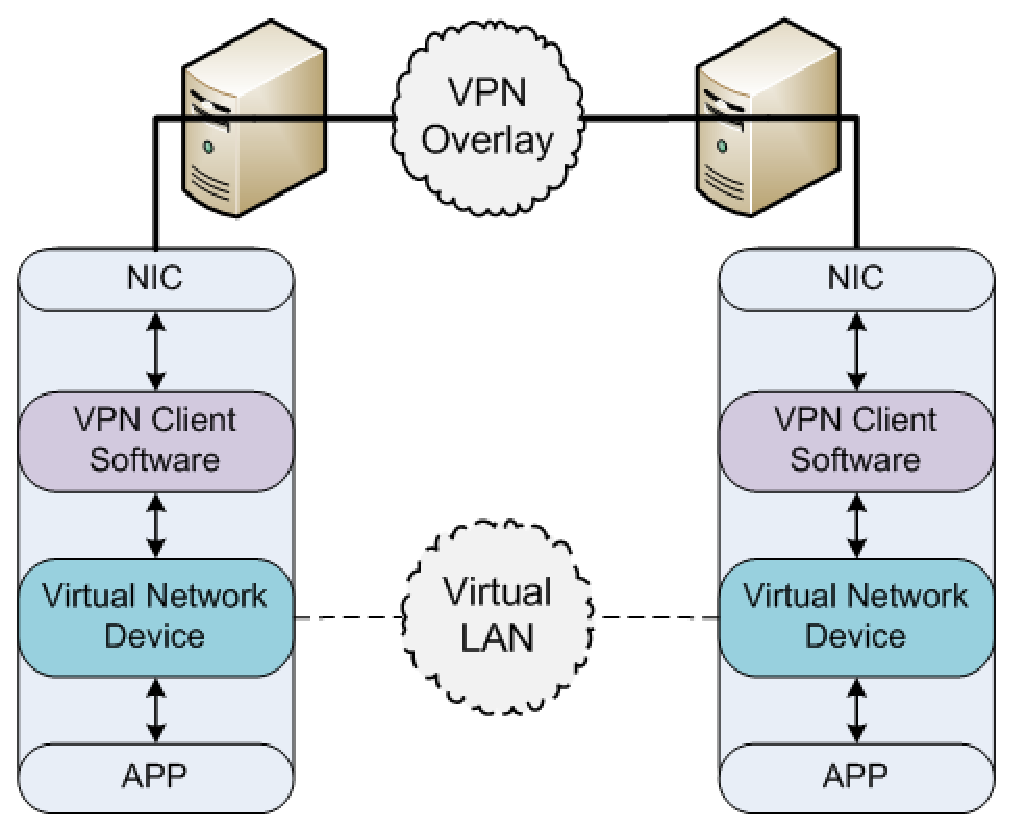
\epsfig{file=figs/vpn.png.eps, width=4in}
\caption[A typical VPN client]{A typical VPN client.  A VN device makes
application interaction with the VPN transparent.  Packets going to the VPN
destination are sent by routing rules to the VN device interfaced by the VPN
client.  The VPN client sends and receives packets from other VPN participants
via the hosts physical network device.}
\label{fig:vpn}
\end{figure}

\chapter{Structured Peer-to-Peer Overlays}
\label{structured_p2p}
This chapter reviews structured overlays and introduces challenges and
proposed solutions regarding connectivity and performance.

\section{Background}
Structured P2P systems provide distributed look up services with guaranteed
search time with a lower bound of $O(\log N)$, in contrast to unstructured
systems, which rely on global knowledge/broadcasts, or stochastic techniques
such as random walks~\cite{unstructured_v_structured}.  Some examples of
structured systems can be found in~\cite{pastry, chord, symphony, kademlia,
can, brunet}.  In general, structured systems are able to make these guarantees
by self-organizing a structured topology, such as a 2D ring (pictured in
Figure~\ref{fig:ring_overlay}) or a hypercube.  Nodes joining an overlay
typically follow these steps:
\begin{enumerate}
\item generate or obtain a unique identification number (node ID) on the
order of 128-bits to 256-bits,
\item connect to a random address from a pre-shared well-known endpoints list,
\item become connected to at least one peer in the list (leaf connection),
\item find the peers closest in the address space to the selected node ID,
\item connect to nodes whose IDs are immediately smaller and / or larger than
itself (neighbor connections),
\item and finally connect to other nodes in the overlay that are not local in
the address space (shortcut connections).
\end{enumerate}

Each node must have a unique node ID; otherwise an address collisions can
prevent nodes from participating in the overlay and can potentially fragment
overlays, preventing them from working properly.  Having node IDs uniformly
distributed assists in providing improved routing in ring-based structured
overlays by requiring fewer shortcut connections than non-uniform distributions.
Each node can generate their own address if they use a cryptographically strong
random number generator.  Another approach for distributing node IDs relies upon
using a trusted third-party to generate and cryptographically sign node
IDs~\cite{secure_routing}.

A node must be connected to closest neighbors in the node ID address space;
optimizations for fault tolerance suggest that for ring topologies the amount
should be between 2 to $\log(N)$ on both sides.  In the case of overlay
disconnectivity especially when related to churn, when a peer does not know the
address of its immediate predecessor or successor and a message is routed
through it destined for them, depending on the message type, it may either be
locally consumed or thrown away, never arriving at its intended destination.
Having multiple neighbors assists in stabilizing the overlay structure when
experiencing churn, particularly when peers leave suddenly without warning.

Overlay shortcuts enable efficient routing in ring-based structured overlays.
The different shortcut selection methods include: maintaining large tables
without using connections and only verifying usability when routing
messages~\cite{pastry, kademlia}, maintaining a connection with a peer every
set distance in the P2P address space~\cite{chord}, or using locations drawn
from a harmonic distribution in the node address space~\cite{symphony}.

Most structured P2P overlays support decentralized storage/look-up of
information by mapping keys to specific node IDs in an overlay.  At a
minimum, the data is stored at the node ID either smaller or larger to the
data's node ID and for fault tolerance the data can be stored at other nodes.
This sort of mapping and data storage is called a distributed hash table (DHT).
DHTs provide the building blocks to form more complex distributed data stores
as presented in Past~\cite{past} and Kosha~\cite{kosha}.

There are two routing mechanisms for communication amongst peers in a
P2P overlay: iterative or recursive.  In iterative routing, the sender of a
packet will directly contact each successive member in a path querying it for
the next until arriving at the destination node, sending the packet directly to
the destination.  In recursive routing, messages are sent through the overlay
via forwarding from one peer to the next until arriving at the destination.
Compared to recursive routing, iterative can be implement more easily.  Though
iterative routing comes with considerable overhead, as each overlay query will
cause $\log(N)$ connections to form.  In addition, iterative routing makes NAT
traversal complicated, as it will require constant traversal mediation and need
to be made quickly; whereas recursive routing provides stable connections due
to a single NAT traversal during the connection phase.

\section{Network Address Translation Hampering P2P Systems}
As of 2010, the majority of the Internet is connected via Internet Protocol (IP)
version 4.  A limitation in this protocol is that there are only $2^{32}$
addresses (approximately 4 billion) available.  With the Earth's population of
over 8 billion and each individual potentially having multiple devices that
have Internet connectivity, the IPv4 limitation is becoming more and more
apparent.  To address this issue there have been two approaches:  1) the use of
network address translation (NAT) to enable many machines and devices to share
a single IP address but preventing bidirectional connection initiation, and 2)
IPv6 which supports $2^{128}$ addresses.  IPv6 does not necessarily imply
direct connectivity as there are no guarantees of NAT disappearing and outbound
only firewalls allowing incoming connections.

When a machine, \textit{A}, behind a typical NAT, \textit{B}, sends out a
packet to an Internet host, \textit{C}, the NAT device translates the packet so
that it appears it is coming from the NAT device making the NAT device a gateway.
When the the packet is sent from \textit{A} to \textit{C}, the source and
destination are listed as $IP:port$ pairs, where the source and destination are
$IP_A:Port_A$ and $IP_C:Port_C$, respectively.  \textit{A} forwards the packet
to \textit{B} who transforms the source from $IP_A:Port_A$ to $IP_B:Port_B$,
where $Port_A$ may or may not be equal to $Port_B$.  This creates a NAT mapping
so that incoming packets from $IP_C:Port_C$ to $IP_B:Port_B$ are translated and
forwarded to $IP_A:Port_A$.

There are a handful of recognized NAT devices as presented in~\cite{stun,
p2p_nats_rfc}.  The following list focuses on the more prevalent types:
\begin{itemize}
\item full cone - all requests from the same internal IP and port are mapped to
a static external IP and port, thus any external host can communicate with the
internal host once a mapping has been made,
\item restricted cone - like a full cone but requires that the internal host
has sent a message to the external host before the NAT will pass the packets,
\item port restricted cone - like a restricted cone but requires that the
internal host has sent the packet to the external hosts specific port before the
NAT will pass packets,
\item symmetric - each source and destination pair have no relation, thus only
a machine receiving a message from an internal host can send a message back.
\end{itemize}

Peers on cone NATs can easily be traversed so long as a third-party assists in
determining the port allocated by the NAT and as a medium for the peers to
exchange this information.  Peers behind symmetric NATs cannot easily
communicate with each other, since there is no relation between remote hosts
and ports and local ports.  Further complicating the matter is that there are
various types of symmetric NATs, having behaviors similar to full, restricted,
and port restricted cone NATs.  \cite{ice} describes methods to traverse
these NATs so long as there is a predictable pattern to port selection.  In
general, these approaches use UDP because of the lack of additional protocol
states, that require replay and ignoring reject methods that occur with the TCP
handshake,  though there is reasonable amount of work describing TCP NAT
traversal such as~\cite{tcp_nat}.  TCP NAT traversal is complicated by stateful
firewalls, or those that watch connections and connection attempts preventing
messages from closed TCP channels from passing through the NAT.  For situations
in which both peers are behind NATs and firewalls that prevent in bound
communication inhibiting NAT traversal, a third party can act as a relay
between the two, known as triangulation or TURN~\cite{turn} (traversal using
relay NAT).

\subsection{NAT Traversal in Structured Overlays}
Structured overlays rely on the principle that any peer can become directly
connected with any other peer in the system.  Thus in order to use structured
overlays on the Internet, they must either be run on publicly accessible
addresses or support NAT traversal.  Even in the case where there is NAT
traversal, occasionally there are Internet routing table breaks and two
peers who should be able to directly communicate cannot.

To date, there exists only one solution, Brunet~\cite{brunet}, supporting
decentralized UDP NAT traversal and limited relays.  To support UDP NAT
traversal, Brunet makes connection attempts bidirectional with peers exchange
all known IP addresses and ports, which it knows directly and from external
overlay nodes.  This enables the traversal of all forms of cone NATs, but
symmetric NATs require iterative rounds of traversal attempts and cannot be
traversed.  If two peers cannot connect, they exchange list of peers, if an
overlap exists, which is highly likely for peers adjacent on the overlay, they
will forward packets through it to each other other~\cite{hpdc08_1}.  This
approach focuses on forming a a correct structured ring not arbitrary two-hop
connections for high performance purposes.  This can be addressed by having
peers connect to each other's neighbor set proactively creating overlap, as
represented in Figure~\ref{fig:relay}.

In addition to exchanging overlap sets, peers also exchange some state of their
connections with the neighbors.  For example, the data shared could be
regarding node stability as measured by the age of a connection and proximity
as measured by ping latency to the neighbor.  When creating overlap or overlap
changes, peers review these metrics to decide which subset of the overlap to
use as a proxy leaving the remaining peers as reserves.

\subsection{Usefulness of Relays}
To determine the value in two-hop overlays as opposed to using the overlay in
restrictive NAT and firewall scenarios, this experiment uses an event-driven
simulator that reuses the code base of the prototype structured P2P VPN to
faithfully implement its functionality using event-driven simulated times to
emulate WAN latencies.  Pair-wise latency in this experiment is set using the
MIT King Data Set~\cite{king_data}, which consists of all-to-all latencies
among 1,740 distributed Internet hosts.  After starting the overlay and after
it has reached steady state, the simulator sends packets amongst all peers to
derive the average all-to-all latency and hop count for messaging in the
overlay.  In the low-latency relay model, each destination node forms a
connection to the source node's physically closest peer as determined via
latency (in a live system by application level ping).  Then this pathway is
used as a two-hop relay between source and node.  Only peers with two hops or
more are analyzed, as a single hop would only benefit under triangular
inequalities, which are not a consideration in this work.

Results are presented in Figure~\ref{fig:simulated_relays}. The network sizes
considered begin at 25 nodes because small networks of sizes 20 and under tend
to be fully connected in the underlying structured overlay.  It is not until
the network size expands past 100 and towards 200 nodes that relays become
significantly beneficial.  At 100 nodes, there is approximately a 54\%
performance increase, whereas at 200 there is an 87\% increase and it appears
to grow proportionately to the size of the pool, demonstrating the performance
advantage of two-hop autonomous relays.

In addition, the autonomous relays functionality were verified in a reference
implementation of a structured P2P VPN using a real system.  The environment
consists of PlanetLab as the public overlay and the Archer environment as the
VPN environment.  PlanetLab~\cite{planetlab} provides a set of over 500
distributed computing nodes all with public IP addresses.  Archer provides grid
computing to computer architecture researchers and consists of over 500 nodes
located at various academic sites.  To ensure that peers under study formed
two-hop connections, a firewall was instantiated preventing direct communication
between the two.  In tests, it was revealed that the overlay was always able to
self-configure a relay; the bandwidth and latency averages and deviations were
2245 Kbit/s $\pm$ 1080 and 58.1 ms $\pm$ 35.5, respectively.

\section{Using Structured Overlays for Direct Communication}
\label{direct_communication}
Applications like VPNs, games, media, and communication can benefit from using
an overlay for discovery and limited communication, though as communication
increases in frequency direct communication may be preferred.  In previous
work~\cite{wow}, the authors describe a method for transparently detecting this
behavior and creating direct links as a result.  In comparing a VPN built on
top of an overlay with a point-to-point direct approach, the VPN using the
overlay has significant overheads due to each IP packet traversing the overlay's
state machine prior to being sent to the VPN, established by
Table~\ref{tab:vpn_eval_comp}.  Thus for high bandwidth applications, this
approach does not scale and costs significant CPU utilization.

Two models in addition to the existing method of communication will be tested
to evaluate methods for obtaining high bandwidth using direct communication
links in overlay networks.  The two new approaches are:  1) Bypass, use the
structured overlay to create and maintain links but placing the application
between the connection and the overlay stack so that the application has first
access to the data, and 2) Separation, use the structured overlay to discover
peers but the application creates and manages its own links using the structured
overlay to coordinate these efforts, presented in Figures \ref{fig:direct_comm_1}
and \ref{fig:direct_comm_2}, respectively.

The first approach benefits from using existing components of the structured
overlay including link creation and maintenance though may still have overheads
due to packets needing to traverse both the application and overlays stack.
This can be addressed by creating a unique thread for processing packets in the
application as well as the overlay stacks.  Since the connections are shared,
this approach will require additional thread synchronization.

The second approach resides external from the structured overlay.  Th
application organizes communication links through the overlay but does not
communicate through it.  Though this is significantly more complicated than the
first solution, the application may be easier to code by reusing existing
overlay code.  Because each component has its own connections and communication
stacks, there is no need to handle synchronization between the overlay and
application.  Essentially, the application will have unfettered access to the
connections it has established.

Evaluation of these approaches will be performed using a VPN application as
described in Chapter~\ref{vpns}.

\section{Overlay-Aware TCP}
\label{tcp}
Communicating large amounts of data reliably and with good performance presents
an interesting challenge when performed through an overlay.  In an overlay,
peers are constantly joining and leaving a network, also known as churn.  During
churn, packets may be lost or misdirected, never arriving at their expected
destination.  Communication via an overlay may pass through many hops and
regardless of the communication protocol used, UDP or TCP, none are aware of
end to end behavior of the overlay focusing only on the point to point
communication between individual peers.  UDP complicates the matter by not
ensuring that communication between two peers is reliable, thus naive use of
UDP does not provide any information regarding the success of transferring a
packet between two peers.

To better understand the effects of overlays on reliable, high throughput
communication, a tool will be implemented to simulate such communication in
overlay environments with various amounts of churn to properly reflect both
dedicated and personal use of the environments.  In dedicated environments, the
behavior will most likely reflect that of the underlying Internet, though this
approach will benefit from proxies that the overlay can create when such outages
occur.  Personal use typically experiences many connections and disconnections,
though those peers that stay connected, tend to stay connected longer than
arriving peers.  The focus of this work will be to investigate existing TCP
solutions used in other networks and determine if there are other potential
solutions and evaluate them.

These results will then be used to implement an overlay-aware system for use in
a real P2P system that will be tested using the PlanetLab overlay.  Likewise with
the simulations, this work will confirm or help correct the modeling results and
provide insights on other potential solutions that may improve performance when
in a real system.

Most common TCP stacks implement a variety of components defined across
several works,\cite{tcp, tcp_congestion, tcp_hp, tcp_mss,
tcp_congestion_notification, tcp_sack}.  Implementing a system accurately
supporting these features could take a significant amount of time with little
research contributions.  There exist a few user space implementations already
support most of these features, such as lwIP~\cite{lwip} and and Userspace
network stack~\cite{unetstack}.  Initially, I will focus on creating a C\#
interface that allows deployment in the Brunet overlay.  If time allows, I will
create a native stack.

\section{Figures and Tables}

\begin{figure}[ht]
\centering
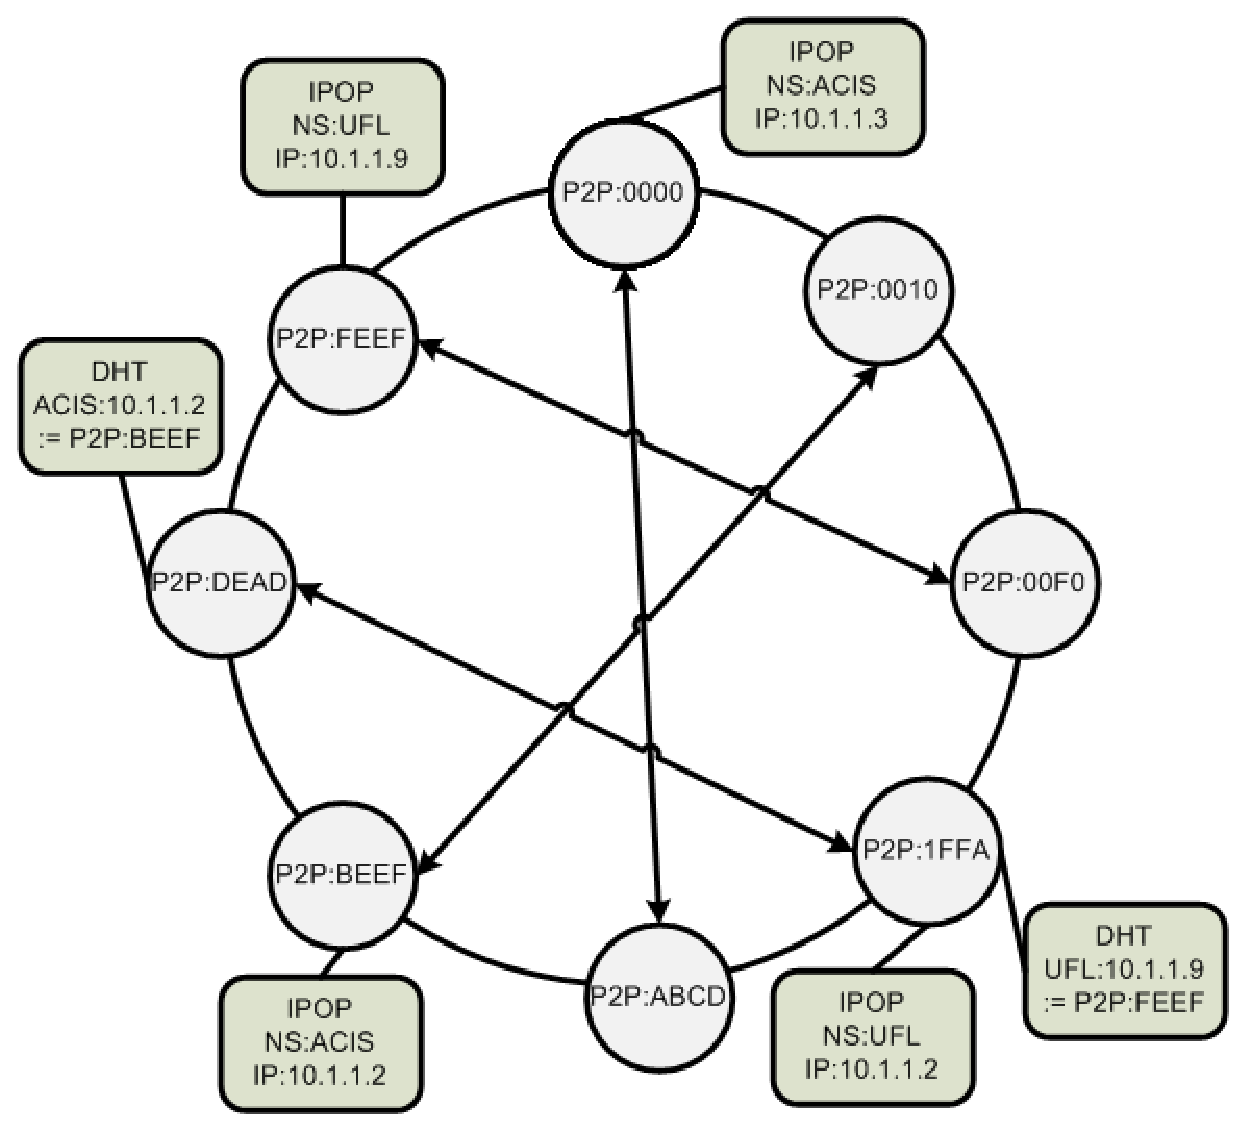
\epsfig{file=figs/ring.eps, width=4in}
\caption{1-D Ring Structured Overlay}
\label{fig:ring_overlay}
\end{figure}

\begin{figure}[ht]
\centering
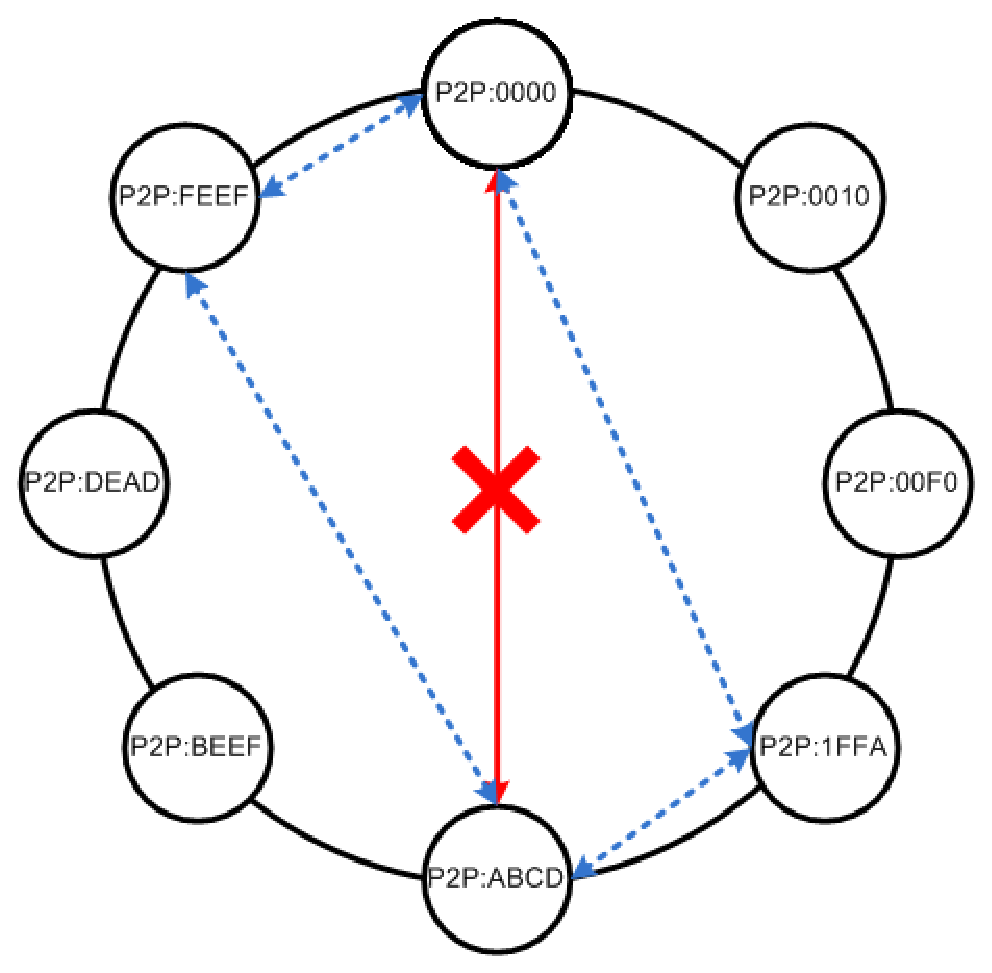
\epsfig{file=figs/relay.png.eps, width=4in}
\caption[Proactive relay creation]{Creating relays across the node address
space, when direct connectivity is not possible.  Two members, 0000 and ABCD, 
desire a direct connection but are unable to directly connect, perhaps due to
NATs or firewalls.  They exchange neighbor information through the overlay and
connect to one of each other's neighbors, creating an overlap.  The overlap
then becomes a relay path (represented by dashed lines), improving performance
over routing across the entire overlay.}
\label{fig:relay}
\end{figure}

\begin{figure}[ht]
\centering
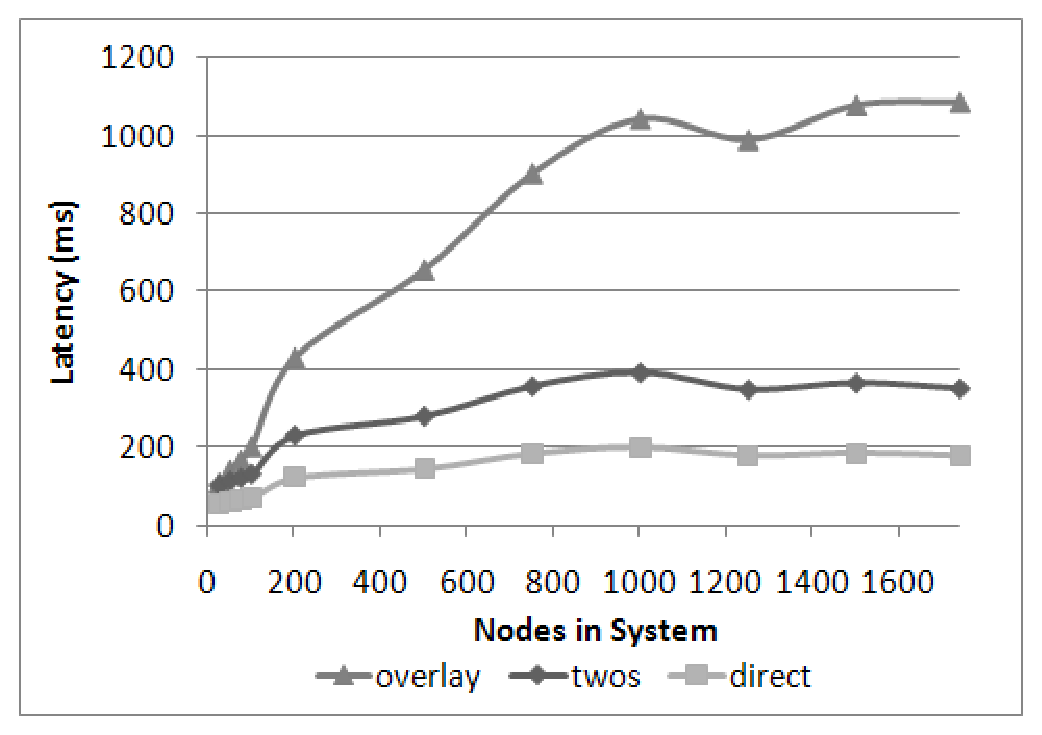
\epsfig{file=figs/relay_motivation.png.eps, width=4in}
\caption[Relay evaluation]{A comparison of the average all-to-all overlay
routing, two-hop relay, and direct connection latency in a Structured P2P
environment, Brunet, using the King data set.}
\label{fig:simulated_relays}
\end{figure}

\begin{figure}[ht]
\centering
\epsfig{file=figs/direct_comm_1.eps, width=4in}
\caption[Direct communication: Bypass model]{Direct communication, Bypass model.
The application reuses the P2P connections but obtains the data first and in a
separate thread.}
\label{fig:direct_communication_1}
\end{figure}

\begin{figure}[ht]
\centering
\epsfig{file=figs/direct_comm_2.eps, width=4in}
\caption[Direct communication: Separation model]{Direct communication: Separation
model.  The application uses the P2P system to discover remote peers and exchange
connection information but forms and maintains connections separate from the P2P
software.}
\label{fig:direct_communication_2}
\end{figure}

\begin{table}[ht]
\caption{VN Stack Comparison}
\label{tab:vpn_eval_comp}
\begin{tabular}{c||c|c|c}
& Latency (ms) & Bwidth (Mb/s) & Mem (KB) \\\hline
Host & 0.27 & 941 & n/a \\\hline
C & 0.34 & 738 & 998 \\\hline
C\# & 0.37 & 716 & 21500 \\\hline
IPOP & 0.52 & 284 & 38312 \\\hline
IPOP sec & 0.75 & 55 & 50976 \\\hline
\end{tabular}
\centering
\end{table}

\chapter{Virtual Private Overlays}
\label{vpo}
While Structured P2P overlays provide a scalable, resilient, and self-managing
platform for distributed applications, their adoption rate has been slow
outside data distribution services such as BitTorrent and eDonkey.  General use
of structured P2P systems, especially in applications targeting homes and
small/medium businesses (SMBs), has been limited in large part due to the
difficult nature of securing such systems to the level required by these users.
Applications in home and SMBs may need a greater level of trust than what can
be guaranteed by anonymous contributors in free-to-join overlays, but many these
users lack the resources or expertise necessary to bootstrap a private P2P
overlays particularly in constrained wide-area network environments where a
significant amount of or all peers may be behind Network Address Translation
devices (NAT).

There are many different P2P applications used in home and small business,
primarily for collaboration and sharing, including data storage, media sharing,
chat, and system maintenance and monitoring.  Applications that currently
provide these functionalities fall into two categories:  anonymous, fully
decentralized free-to-join P2P systems and distributed systems with P2P
communication that rely on a third party to provide discovery and management.
While using a third party service provides a desirable level of trust for many
users, it has significant drawbacks such as vendor lock-in, which may result in
lost data, down time, and scalability constraints.

An example of a useful small business application that falls into the latter
category is LogMeIn's~\cite{logmein} software products LogMeIn Pro and Hamachi.
LogMeIn Pro allows users to remotely manage and connect with their machines so
long as they are willing to use LogMeIn's software and infrastructure.  Hamachi
allows users to establish decentralized VPN links using centralized session
management.  Both applications assist in the remote maintenance and monitoring
of computers without requiring the user to implement the networking
infrastructure provided by LogMeIn.

Some examples of P2P applications for homes and small businesses in development
are P2PSIP~\cite{p2psip} and P2Pns~\cite{p2pns}.  P2PSIP enables users to
initiate, through decentralized means, visual and audio communication, while
P2Pns allows users to deploy a decentralized naming service.  Both applications
allow users to contribute and benefit from all members of the system without
the regulation of a third party, but lack the ability to allow users to
centrally secure and manage their own subset of the systems.

Distributed data store applications like Dynamo~\cite{dynamo} and
BigTable~\cite{bigtable} have the ability to store data using a completely
decentralized system.  Though these systems are highly scalable and fault
tolerant, the software uses an insecure overlay.  Therefore all instances
need to run in a secure environment, whether that is in a single institution
or across a largely distributed environment using a VPN.

This chapter reviews security issues and current examples of security in P2P.
Using the motivation of user centric and friendly systems, I present a method
for users to create their own secure, private overlays using the same core
overlay primitives as public overlays without the constraints imposed on them
by lacking dedicated, public resources through the use of a shared,
free-to-join public overlay.

\section{Security Issues in Structured Overlays}
While there has been much research~\cite{secure_routing} in securing overlays
through decentralized mechanisms that attempt to prevent collusion known as
a Sybil attack~\cite{sybil}, these mechanisms do not create private overlays.
One approach mentioned does provide a natural lead into such environments by
using of a pay-to-use service to mitigate the chances of an overlay attack,
whereby the pay to use service uses a CA to sign node IDs.  The work does not
describe how to efficiently implement such a system.  Other
projects~\cite{stone, tor} combine trusted overlays with anonymous members,
though it could be reasonably argued these services are not applicable to small
or medium business, which would prefer to have a private overlay.  None of the
works focus on how to apply such models to systems that are constrained in
network connectivity, e.g. by NATs.

\section{Secure Overlays}
\label{secure_overlays}
In recursive overlays, there are two forms of overlay communication:
\begin{itemize}
\item \textbf{Point-to-point (PtP)}:  Direct connections between peers in an
overlay, such as a UDP, TCP, or relay connecting two peers.  In an iterative
system, all messages are PtP.
\item \textbf{End-to-end (EtE)}:  Messages passed through an overlay from
peer to peer, used typically for application communication such as DHT queries.
\end{itemize}
Iterative overlays do not distinguish between the two forms of communication as
all communication is directly between two peers and never indirectly
communicated unless relays are used.

Securing communication in overlays using iterative routing without relays and
static IP addresses can easily be done using TLS~\cite{tls} or DTLS~\cite{dtls}
with certificates bound to the node's IP address.  Similarly PtP can be secured
in recursive overlays with static address.  Including relays, NAT traversal, or
EtE in recursive overlays complicates the issue.  NAT traversal cannot must
bind the certificate to something other than the peers IP address. Relays and
EtE routing require communicating through indirect communication and existing
security libraries are built on top of sockets and thus are not applicable in
these environments.  Furthermore, overlays are not reliable environments and
thus without a reliable overlay primitive TLS cannot be employed.  DTLS can
be applied because it supports lost and out of order messages, though the
implementation must support usage without a socket.  In this section, I discuss
how to bind security protocols and a certificate model to an overlay system
addressing the issue of applying DTLS to overlays and binding certificates to
individuals even in NAT environments.

The key to my approach is the abstraction used in the communication layer,
making EtE and PtP traffic appear identical. In this approach, all messages
are treated as datagrams, which are sent over abstracted senders and receivers
as filters illustrated in Figure~\ref{fig:senders_receivers}.  This allows use
of secure tunnels over these links with no application changes.

Exchanged certificates need a mechanism to verify authenticity.  Like an
Internet browser, this verification should happen automatically with no user
intervention.  Typically for SSL-derivatives, the certificates have the owner's
IP address or domain name as part of the certificate's common name field.  In
the prototype system, the certificate is bound to each individual node ID.
That way, a single certificate cannot be used for multiple peers in the
overlay, making it difficult for an adversary to launch Sybil attacks.

\subsection{Forming the Connection}
In overlay systems, a peer's connection manager requests an outgoing
connection to another peer in the system.  This triggers the creation of a
socket (UDP or TCP), which is wrapped in the abstracted sender and receiver
models.  The abstracted models arrive into the security handler, which
authenticates in both directions and creates a secure session.  The session is
wrapped in the same abstracted model and presented to the overlay system as a
direct connection to the remote peer.  To keep the system abstract, the security
model and the wrapped sockets know nothing about the overlay, and so the overlay
should verify the certificate to ensure identity.

Because EtE communication is application-specific, it requires a slightly
different path.  For that purpose, users are able to obtain a secure EtE
sender through an instance factory, allowing multiplexing of secure senders for
multiple applications as well as PtP communication.  Once an application
requests the sender, the module passes a sender / receiver model to the
security handler, like in the PtP process.  Once the security initialization
has completed, the resulting sender / receiver is verified automatically for
proper identity.  If that succeeds, messages sent using the EtE sender will
arrive at the remote party, decrypted and authenticated by the security
handler, and delivered to the overlay application, who will deliver to the
remote party's handler for such messages.  Since overlay applications will be
sending and receiving unencrypted as well as encrypted EtE traffic, the handler
must verify that the packet was sent from a secure end point.  This assumes
that an application using an overlay has already implemented verification of
node ID to some application mapping.  For example, an application could be
aware that node ID X maps to user Y, therefore if a secure message coming from
node ID Z says that it is user Y, an application should drop the packet.

\subsection{Datagram Constraints}
UDP is a connectionless protocol, enabling applications that use it to easily
become victims of denial of service attacks.  This is because packets sent to
the receiver can have a spoofed source address, unless the outgoing gateway
prevents this from occurring, egress filtering.  For each spoofed attempt, the
security system maintains state, which might eventually be overloaded.  In TCP,
this is hampered due to the three message handshake, which verifies that a
source address is not spoofed, prior to creating security state for the
connection.  To reduce the potential of these spoofing attacks prior to
establishing a secure connection, DTLS (like Photuris~\cite{photuris}) uses a
stateless cookie for each remote peer.  In DTLS, the cookie is usually based
upon the remote peer's IP and the current time.  In prototype model, which
deals with abstracted systems and IP addresses are likely to be NAT-translated,
this approach does not work.  Though for PtP, it is possible to use the address
and port from which the remote peer last sent a message from.  For EtE traffic,
the node ID can be used for cookie calculation.  Because we are building on
existing senders and receivers that already have state, we use the object's
memory pointer or hash value instead, though this leads us down a similar path
of denial of service found in TCP SYN attacks.

\subsection{Implementation}
To provide security, I investigated two approaches:  reusing OpenSSL's DTLS
implementation and a platform-independent approach similar to DTLS using C\#
and cryptography routines provided by .NET.  A constraint in the development is
that EtE communication must be able to be secured, which could be enabled by a
filter approach using memory buffers instead of sockets.

Implementation of an OpenSSL DTLS filter was non-trivial, as documentation is
sparse providing the possibility for varied approaches.  Traditionally, DTLS
uses the DGRAM (datagram) BIO (I/O abstraction) layer, which provides a reliable
UDP layer.  To support the filter behavior to support both EtE and PtP traffic,
one memory BIO was used for incoming traffic and another for outgoing traffic.
Memory BIOs provide pipes using RAM: data written to the BIO can then be read
in a first in, first out ordering.  Incoming messages written to or outgoing
messages read from the DTLS read or write BIOs, respectively, are either
encrypted data packets or handshake control messages.  Sending and receiving
clear text messages occur at the DTLS SSL object layer.  The pathway for
sending a clear text packet begins with the user performing an SSL\_write
operation, retrieving the encrypted data by performing a BIO\_read on the write
BIO, and sending the data over the network.  At the remote end, the packet is
passed to the SSL state machine by performing a BIO\_write on the incoming BIO
followed by a SSL\_read; the result will be the original clear text message.
This process also needs to handle control messages; we provide clear context in
Figure~\ref{fig:dtls_filter}.  As an aside, OpenSSL supports a SSL filter
BIO, though it will not work for this purpose as BIOs that are inserted are
expected to have two pipes, like a socket or two memory buffers.  Also the only
benefit of using the filter BIO would be that it manages auto-renegotiation,
which can be implemented in user code by monitoring time and received byte
count.  Other operations such as certificate verification and cookie generation
are handled by SSL callbacks, which hook into the security framework.

OpenSSL is a de-facto standard, with US federal government approved code (FIPS)
and platform portability, though during my development involving the platform I
experienced a few issues.  The portability provided by OpenSSL is limited to
API (Application Programming Interface) and not ABI (Application Binary
Interface), which requires a platform-specific library be either installed or
distributed with the application.  Whereas the purpose in using C\#, like Java,
is that a single binary can run on any platform.  To use unmanaged libraries
from a managed language requires a marshaling wrapper to handle the
translation; there is such a wrapper for OpenSSL~\cite{openssl.net}.  A
constraint we found when using the library was the naming of the OpenSSL
libraries was not consistent across platforms and, additionally, Windows lacked
a formal installation method.

In using the OpenSSL library with DTLS, in version 0.9.8k, renegotiation of
security parameters  was broken and would result in a deadlocked DTLS session,
whereas in 1.0.0-beta3 (the latest released beta) DTLS renegotiation worked;
however, it would often segmentation fault.  These issues were the motivation
for the creation of a platform independent security architecture similar to
DTLS written in C\#.  To provide for flexibility between the two approaches,
I created a security overlord that treats each approach like a filter.
Treating each implementation as a filter allows incoming control and data
messages to be pushed into the object and data and control messages to be
pulled out of the object.  While I believe OpenSSL's DTLS to be a superior
choice due to its prevalence and being well studied, it is non-trivial to make
available for all platforms.  Because my goal is to provide a safe yet easy to
use the overlay package, I leave the decision up to the user which protocol to
use.   I believe those interested in testing the system will start with the
.NET security stack and migrate to the OpenSSL DTLS stack.


% The handshake used is shown in Figure~\ref{fig:dtls}.
%\begin{figure}[h]
%\centering
%\includegraphics[width=2.75in]{in_progress.eps}
%\caption{DTLS Handshake}
%\label{fig:dtls}
%\end{figure}

Since symmetric keys work on limited block size, they use modes of operation
to encrypt or decrypt large sets of blocks.  Because DTLS uses an unreliable
transfer mechanism, each message should be able to be decrypted without the use
of previous messages.  As suggested in the DTLS paper, we used cipher-block
chaining (CBC) with a new initialization vector (IV) for each message.  During
analysis of the C\# implementation, it was apparent that generating an IV was
expensive but the initialization of an additional CBC state machine was even
more.  To reduce these costs, the sender always uses the same CBC state machine
and prepends the last cipher-block to the beginning of the next message.  Upon
reception, a receiver compares the prepended message to a cache of CBC state
machines stored by the current state, if there is a match, then the CBC state
machine can be used, otherwise, if the packet is received out of order the
receiver can start a new CBC state machine to decrypt the packet.  This issue
does not appear in the OpenSSL implementation of CBC.

\section{Private Overlays}
\label{private_overlays}
The main components involved in starting and maintaining a private overlay
are 1) dissemination of the security credentials and its name, 2) connecting
with and storing data in the public overlay, and 3) discovering and connecting
with peers in the private overlay.  Step 1) can be application-specific; we
propose a generic interface that is useful in many applications, through the
use of groups as described in Section Section~\ref{group_overlays}.  For 2),
we presume the usage of a structured overlay as described in
Chapter~\ref{structured_p2p}.  In this section, we discuss 3), the steps
involved in creating and connecting to a private overlay after the user has
obtained group information and has connected to a public overlay.

To connect with and create a private overlay, the application performs the
following steps, as depicted in Figure~\ref{fig:private_overlay_states}: 1)
connect to the public overlay; 2) store node ID in the public overlay's DHT at
the private group's key; 3) query the public overlay's DHT at the private
group's key; 4) start an instance of the private overlay with the well-known
end points being the node IDs retrieved from the DHT; and 5) upon forming a
link with a member in the private overlay, the node follows the standard
approach for linking to neighbors and shortcuts but using secure PtP links to
restrict connections to members of the private overlay.

While a node does not need to maintain membership in the public overlay once
connected with the private overlay, it will benefit the private overlay for it
to do so.  If the peer remains in the private overlay, other peers can discover
the node while following the same set of steps and, for NAT traversal purposes,
as discussed in the next paragraph.  Because the public overlay and its DHT
provides a means for discovery, nodes should maintain their node ID in the public
overlay's DHT.  If the DHT employs a lease or soft state system, while online
the node must renew the lease prior to expiring.

During the formation of the private overlay, peers may find that they are
unable to form direct connections with other members of the private overlay
even while using STUN based NAT traversal.   To address this problem, peers can
1) use TURN NAT traversal in the nodes overlay as in Chapter~\ref{structured_p2p}
or 2) use the public overlay as an extra routing massive TURN infrastructure.
The TURN NAT traversal technique has both peers connect with each other's near
neighbors in order to form a 2-hop connection with each other.  The 2-hop route
can either be enforced through a static route or through EtE greedy routing.
Due to the abstractions in the system, the public overlay can be treated as
another mechanism to create PtP links, thus while packets may use EtE routing
on the public overlay, the private overlay nodes treat it as a PtP connection
thus all communication is secured.  This approach can be further enhanced by
allowing the private overlay to apply the TURN NAT traversal technique to the
public overlay.  To do this, the private overlay must be capable of requesting
a direct connection between its node and the remote peer in the public overlay.
This would trigger the eventual creation of a 2-hop relay connection as
presented in Figure~\ref{fig:overlay_relay}.

%Another concern we address is the cost of having to maintain additional
%connections for each additional private overlay.  For this, we propose the use of
%{\em pathing}, which multiplex a single UDP or TCP socket to support multiple
%overlay nodes.  This model is supported because of the abstraction done on
%senders and receivers.  Thus a UDP or TCP connection can be easily wrapped 
%inside an arbitrary packet, in this case, a pathing connection.  Upon sending
%a packet, the message is prepended with path information.  When the remote side
%receives a packet, it parses and removes this pathing information and relays it
%to the appropriate receiver, i.e., overlay node.  We validate this approach in
%Section~\ref{pathing_evaluation}.

If overlays are small and have significant churn, it is highly likely that data
stored in the overlay's DHT to be lost.  This can be improved by also supporting
broadcast in the private overlay.  In this model, each peer acts as a storage
point for all data critical to itself.  If another peer cannot successfully
find data stored at a specific key in the overlay, it can make use of broadcast
over the entire overlay in an attempt to find the result.  The technical details
of Brunet's broadcast implementation are described in Appendix~\ref{broadcast}.
As the broadcast involves forwarding packets, the revoked peer will receive
a revocation notice but the forwarder does not include it in the calculations
of bounds and thus they are never responsible for forwarding the revocation
onwards.

During evaluation, it was discovered that in certain cases the private overlay
would not form a proper well-formed state but rather more than one distinct
overlays, creating a partitioned overlay.  The underlying issue was that the
partitioned overlays believed they were in a well-formed state and thus never
reviewed the DHT list to determine if there were peers that should be their
neighbors.  This caused the overlay to remain fragmented until either a new
peer joined or enough peers left causing the nodes to believe they are in a
non-well-formed state and require bootstrapping links.  The issue stemmed from
significant churn, especially during bootstrapping of significant new nodes in
the public overlay, causing entries in the DHT list can become partitioned,
with each set of nodes potentially seeing different lists.  Eventually the
lists stored in the DHT become consistent, but at that point, the overlay would
have already been partitioned.

To proactively solve the partitioning issue, the node performs the following
steps: 1) continuously query the DHT;  2) upon receiving the DHT query result,
the node determines if there is a peer with whom it should be connected to
such as that it is closer in the address space than any of its current neighbors;
3) form a connection with that peer; and 4) the system should automatically at
this point in time realize the network fragmentation and heal itself.  In the
prototype system, this involved creating a bootstrapping connection with the
peer.  Upon a successful connection, the system automatically causes the
networks to heal.

\section{Group Overlays}
\label{group_overlays}
Establishing trusted links in a P2P system can easily be achieved via a PKI
model, where a centralized CA signs all client certificates and clients can
verify each other without CA interaction by using the CA's public certificate.
However, setting up, deploying, and then maintaining security credentials can
easily become a non-negligible task, especially for non-experts.  Most
PKI-enabled systems require the use of command-line utilities and lack methods
for assisting in the deployment of certificates and policing users.  In order
to facilitate use in real systems with non-experts, it is important to have an
easy to use framework.  A solution to this issue is a partially automated PKI
reliant on a redistributable group based web interface, where each group has
its own unique CA independent of other groups.  Although this does not preclude
other methods of CA interaction, experience has shown that it provides a model
that is satisfactory for many use cases.  

\subsection{Joining the Group Overlay}
Membership of an overlay maps a set of users as a group, easily enabling PKI
models via group infrastructures.  Using this system, a user can host an
individual or multiple groups per web site.  The creator of the group becomes
the default administrator, and users can request access to the group.  Upon an
administrator approving, users are able to download configuration data
containing overlay information and a shared key.  The shared key is used by the
overlay application to communicate securely with the web interface to uniquely
identify the user allowing the application to securely send certificate
requests and receive signed certificates.  By default, the web site
automatically signs all certificate requests, though it is not limited to this
model.  Two other approaches are 1) require the user to submit a request and
wait for an administrator to verify each request and 2) set a maximum amount of
automatic request signings then requiring administrative approval for more.

As stated in Section~\ref{secure_overlays}, the certificate request is bound
to the application's node ID, which can be generated by the CA or the
application.  Additionally in the group system, the certificate also contains
the user who made the request and the group for which the certificate is valid.
Not only does this ensure that a single certificate can only be used for each
node instance, but it reduces the amount of state necessary to revoke a user
from a system.  Specifically, to revoke a user, the CA would only need to
provide a signed revocation notice containing the user's name and not every one
of the previously signed certificates.

Upon receiving a signed certificate, the application can connect to the overlay
where all PtP traffic will be secured and, optionally, so can EtE traffic.  It
is imperative that any operations that involve the exchanging of secret
information, such as the shared secret, be performed over a secure transport,
such as HTTPS, which can be done with no user intervention.

\subsection{Leaving or Being Removed from a Group}
In the group environment, administrators also have the ability to remove users
from the group.  In turn, this will cause a user revocation, which is detailed
more in Section~\ref{revocation}.  In addition, users that leave the group
should also have their certificates revoked, attempting to revoke a user's
certificates after they have left the group can be a difficult undertaking
if the group interface no longer has memory of those users.  Once a user has
been revoked, the revocation should not be reversed as ensuring that a user
has received a notice to ignore an already deployed revocation message can be
difficult to verify in a live, decentralized  system.  Instead, revoked or
users who have left should be forever listed in the group and if the users are
welcome back again, they should create new accounts.  Alternatively, unique
numbers could be assigned to a user, thus an account number and not a username
could be revoked.

\section{User Revocation}
\label{revocation}
Unlike decentralized systems that use shared secrets, in which the creator of
the overlay becomes powerless to control malicious users, a PKI enables the
creator to effectively remove malicious users.  The methods that we have
incorporated include:  a user revocation list hosted on the group server,
DHT events requesting notification of peer removal from the group, and
broadcasting to the entire P2P system the revocation of the peer.

A user revocation list offers an out-of-band distribution mechanism that cannot
easily be tampered, whereas communication using the overlay can be hampered
by Sybil attacks.  The revocation list is maintained on the Web site and updated
whenever an administrator removes a user, or a user leaves the group.
Additionally it can be updated periodically so that a user can verify that the
revocation list is up to date.

However, because the user revocation list requires centralization, users should
not query it prior to every communication nor periodically during conversations.
In addition to support for polling the revocation list, the use of the DHT and
broadcast provides active notification of user revocation.  Revocation through
the DHT method allows a peer to request notification if another peer is revoked
from the group.  To subscribe for this notification, the peer inserts its node
ID at the peer's revocation notification key, which we represent as a hash of
its node ID.  Upon revocation, the CA will first insert a revocation notice at
this key and then query the key for all node IDs notifying each of them of the
revocation.  The insertion of the revocation notice handles a race condition,
where a peer may insert its ID but never receive a notification.  Thus after
inserting the request for notification upon revocation, the peer should ensure
that a revocation has not occurred by querying the DHT to verify the
non-existence of a CA revocation.

When the group is securing PtP traffic, the DHT approach does not effectively
seal the rogue user from the system until all peers have updated the revocation
list.  A peer may continuously connect to all peers in the system until they
have all queried the DHT key prior to verification.  Due to this issue, we 
consider an additional model in the group overlay: an overlay broadcast, ensuring
that all peers in the private overlay do know about the revocation.  

Because the security framework is based on PKI, another approach that is also
supported is the use of certificate revocation lists (CRL) found in most CA
systems.  The advantage of a CRL and revoking individual certificates is the
ability to remove a subset of a user's node, particularly useful in the case
that the user was not malicious but that some of their nodes had been tampered
or hijacked.

\section{Applications}
\label{applications}
This section presents some applications and potential ways to configure them
to use a private overlay.  The applications investigated include chat rooms,
social networks, VPNs, and multicast.  The key to all these applications is that
users can easily host their own services and be discovered through the use of
a NAT-traversing, structured overlay network.

\subsection{Chat Rooms}
Chat rooms provide a platform for individuals with a common interest to find
each other, group discussion, private chat, and data exchange.  One of the most
popular chat systems for the Internet is Internet Relay Chat (IRC).  As
described in~\cite{irc}, IRC supports a distributed tree system, where clients
connect to a server, and servers use a mixture of unicast and multicast to
distribute messages.  The issues with IRC are documented by~\cite{irc_arch},
namely, scalability due to all servers needing global knowledge, reliability due
to connectivity issues between servers, and lack of privacy.  Private overlays
could be extended to support the features of IRC and potentially deal with these
inherent issues.  Each chat room would be mapped to a private overlay and the
public overlay would be used as a directory to learn about available chat rooms
and request access.  Structured overlays do not require global knowledge and can
be configured to handle connectivity issues.  Additionally, IRC by default uses
clear text messaging and even if security is used a server will be aware of the
content of the message, two issues resolved by using PtP security in a private
overlay chat room.  

\subsection{Social Networks}
Social networks such as Facebook and MySpace provide an opportunity for users to
indirectly share information with friends, family, and peers via a profile
containing personal information, status updates, and pictures.
Most social network structures rely on hosted systems, where they become
the keepers of user data, which creates privacy and trust concerns.  Private overlays
can remove this third party, making users the only owner of their data.  For this
model, we propose that each user's profile be represented by a private overlay
and that each of their friends become members of this overlay.  The overlay will
consist of a secured DHT, where only writes made by the overlay owner are valid
and only members of the overlay have access to the content stored in it.  In
addition to bootstrapping the private overlays, the public overlay would be
used as a directory for users to find and befriend each other.  For fault
tolerance and scalability, each user provides a copy of their profile
locally, which will be distributed amongst the private overlay in a read-only
DHT, therefore, allowing the user's profile to be visible whether they are
offline or online.  Each user's social network would than consist of the
accumulation of the individual private overlays and the public overlay.
This is covered in greater depth in Chapter~\ref{spo}.

\subsection{P2P VPNs}
As will be described later in Chapter~\ref{vpns}, private overlays enable P2P
VPNs.  The most common type of VPNs are centralized VPNs like OpenVPN, which
requires that a centralized set of resources handle session initialization and
communication.  Another approach taken by Hamachi and many others is to
maintain a central server for session initialization but allow communication to
occur directly between peers and providing a central relay when NAT traversal
fails.  Using a structured private overlay allows users to host their own
VPNs, where each VPN end points is responsible for its own session
initialization and communication.  The private overlay also provides mechanisms
for handling failed NAT traversal attempts via relaying.

\subsection{Multicast}
The topic of secure multicast has been a focus of much research.  Using an
approach similar to CAN~\cite{can_multicast}, a virtual private overlay forms
a ring where all nodes are members of the multicast group with the additional
feature that the broadcaster can trust that the audience is limited to those
in the overlay.  The main advantage of such multicasting technologies would be
for wide-area, distributed multicast.  Examples of such services include light
weight multicast DNS / DNS-SD (service discovery), as well as audio and video
streaming.

\section{Evaluation of Private Virtual Overlays}
In this section, I evaluate the time required to create and join private virtual
overlays using a three different environments:

\begin{itemize}
\item \textbf{Network Modeling}: Modeling of the system is done through an
application that generates a structured overlay with the usual dimensions found
in deployed steady state systems: a system of size N with each peer having 3
near neighbors on both sides and $O(.5\log N)$ shortcuts.  The modeler creates a
fully connected system where shortcuts are optimally chosen based upon their
location in the node ID space using a harmonic distribution.  Brunet routing
code can then be used on a fully generated overlay to model the number of
nodes visited and message latencies.  Delays between nodes was generated using
the MIT King data set~\cite{king_data}.  The MIT King data set consists of
latency between DNS servers distributed globally on the Internet.  Since the
MIT King data set only covers 1740 nodes, peers in larger networks are
randomly distributed in the address space placing multiple nodes at the same
``physical'' location when necessary. The overhead due to security was modeled
by adding 3 round-trip latencies to prior to all connection processes. This
models the behavior of the 6-message DTLS handshake used in the deployed code
base.
\item \textbf{Simulations} The approach described above estimates time based
upon a model that reuses the core routing algorithm of the overlay code but
does not fully capture the dynamics of the overlay such as state machines
involved in connection handling.  To allow complete evaluation of the prototype
software stack, a simulator using event-driven time that faithfully reusing the
entire overlay code base including routing, security, DHT, and connection state
machines is used.  This allows the verification of correct behavior in the
overlay prior to testing out on real systems, such as PlanetLab, as well as to
perform experiments in a controlled environment, which simplifies the
evaluation while still retaining the effects of a wide-are distributed system.
This environment, like the network modeler, employs the MIT King data
set~\cite{king_data} for pair wise latency between peers.  Because the network
modeler is very light weight, it can model more than 100,000 peers using a
single computer; however, the simulator reuses the entire overlay software and
can only simulate around 1,000 peers.
\item \textbf{PlanetLab} PlanetLab~\cite{planetlab} is a consortium of research
institutes sharing hundreds of globally distributed network and computing
resources.  PlanetLab provides a very interesting environment as there is
constant unexpected churn of machines due to the extreme load placed on the
resources and unscheduled system restarts.  Complementary to simulation,
PlanetLab gives a glimpse of what to expect from the P2P software stack when
used in an actual environment subject to higher variance due to resource
contention and churn.  Due to the time required and complexities in working with
PlanetLab, it is used only for a limited number of experiments with focus on the
time required to join a private overlay.
\end{itemize}

\subsection{Connecting to the Private Overlay}
This experiments provides light on the overall time required for a node to
connect to the public overlay, and then for a subsequent paired node to connect
to the private overlay.  Connected implies that a node has with the nodes whose
IDs are closest in the ring (i.e., neighbors with IDs both smaller than and
larger than the node who is joining).  The results of this experiment show the
time it takes to connect to a public overlay, query the DHT for private overlay
information, and then connect to a private overlay with and without security.

To summarize the connection process, the public node is started.  Upon becoming
connected, the private node will insert into the DHT its private overlay
information using an automated lease extender.  Afterwards, it queries the
public overlays DHT for information regarding other nodes.  Upon successful
retrieval, the results are appended to the list of potential nodes from which
the bootstrapping state machine pulls addresses from during the early
connection phase.  The test terminates when the private node reaches a
connected state.  The private node is started after the public node due in part
to earlier experiments, in which it was noted that starting the public and
private nodes at the same time took longer due to the state machines in the
private node using exponential time back-offs of up to a minute when there
were no nodes in the bootstrapping node list.

For PlanetLab, several overlays with random distribution of private nodes were
created.  Starting from a base public overlay of 600 nodes on distinct PlanetLab
hosts, each node randomly decides whether or not to join the private overlay in
order to obtain private overlays consisting of 5 to 600 members.  Crawling the
overlay provided the actual amount of nodes in the private overlay.  The
experiment entailed connecting to the ring from the same physical location 100
times using a different node ID each time, causing the node to join different
peers and creating a distribution of connection times. During this process, the
time it took for the public node and private nodes to connect is measured.  
Experiments were started after waiting an hour to ensure the system was fully
connected or reached steady state.  This is a conservative value; experience
suggests that overlays run on PlanetLab with various sizes can form a complete
ring in the order of minutes.

Simulation follows similar steps though with the peer count tightened to exact
amount of peers in both the public and private overlays.  The public pool
contains 700 nodes and the private pool 2 to 300 members.  After waiting for
the overlay to become fully connected and additional 60 simulated minutes is
executed to ensure steady state.  At which point, an additional public node
with a matching private node are added to the system.  The results measures are
the time required for them to become connected.

The modeler repeats the steps done for the simulation, though with network
sizes up to 100,000 nodes.  To verify the modeling evaluations are correct,
PlanetLab and Simulation results were tested in addition to much larger
networks, as shown in Figure~\ref{fig:single_join_mod}.  Timing is based upon
the typical connection steps when connecting to the public overlay, querying
the DHT, and then connecting to the private overlay using this process as the
basis for evaluation.

The results, Figures~\ref{fig:single_join},~\ref{fig:single_join_mod} are well
correlated with near identical slopes.  In all cases the time to become
connected with the private overlay remains reasonable and scales logarithmically
as network size grows.  Connection times differ amongst the sets, in the case of
the Simulator all the state machines are at the maximum wait delay due to lack
of churn in the system, whereas PlanetLab has limited overhead due to this
delay, and the modeler does not worry about state machine state, churn, or bad
connection attempts.  An important result is that PtP security does not
significantly add to time to joining the overlays, most likely due to the
majority of the time being occupied by overlay routing.

\subsection{Instantaneous Pool Creation}
\label{mass_join}
This experiment determines the amount of time required to bootstrap a private
overlay including their matching public overlay nodes using an existing network.
The experiment starts with a public network size of 200 public nodes with
various amounts of additional nodes that also have a private overlay pair.
Because PlanetLab is difficult to control in terms of attempting to start 200
public nodes simultaneously and ensuring that they do not restart
mid-experiment, this experiment was run using the simulator.  

Figure~\ref{fig:big_join} presents the results with and without security for
various sized networks.  The results present a slightly different picture than
the previous experiment.  In this case, there is a slightly logarithmic growth
to the time it takes to complete an overlay.  As in the previous test, the use
of security has a small relative impact on the overall time to form the ring.

\subsection{Measuring Bandwidth}
This experiment reuses the overlay bootstrapped in the previous experiment and
measures bandwidth for 60 minutes, the 60 minutes after the overlay is
well-formed.  Reusing the simulation results changes has no effect on the
results of this experiment and cuts down on the most expensive part of the
procedure, the bootstrap phase.  The results are shown in
Figure~\ref{fig:vpo_bandwidth}.

As shown in Figure~\ref{fig:vpo_bandwidth}, when comparing the querying of the DHT
using static and dynamic timers, the static timer's bandwidth is dominated by
DHT queries.  Since the system is at steady state, i.e., no new nodes in the
system, only a single DHT query is made using dynamic timers.  In both cases,
the time to form a complete ring as performed in Section~\ref{mass_join} is the
same. The dynamic timer causes bandwidth to grow slower than a logarithmic pace.
Given that the bandwidth used grows slowly, it appears that overlays in general
use negligible amounts of bandwidth and that even using security does not
increase it significantly.

In regards to selecting a proper timeout, it can logically be surmised that
if an existing public and private overlay were going through heavy churn,
there will always be a base of nodes connected to each other.  If because the DHT
is currently fragmented, a new node forms a partitioned private overlay, the node
should eventually and quickly find out about the original overlay and reform
the split overlays due to the continuous queries.  The advantage of the dynamic
timeout is that it places the weight for fixing ring partitions
on the nodes that created them rather than the older more stable nodes. 

\subsection{Evaluating Revocation Implementations}
\label{evaluation_revocation}
Figures~\ref{fig:revocation_sim} and \ref{fig:revocation_mod} present the time
required and network traffic to perform a revocation using the simulator and
modeler, respectively.  The values were determined by setting the estimated
average size of a revocation to 300 bytes , which includes information such as
the user's name, the group, time of revocation, and a signature from the CA's
private key.  To evaluate the cost in simulations, the bandwidth was measured
for 30 seconds that included the revocation and 30 seconds where there was no
activity.  The time sample was chosen because it represented the smallest
amount of time that would contain a representative steady state bandwidth but
also make the cost of revocation obvious.  The modeler only contains total
bytes required for the operation because no connection based steady state
behavior is modeled.

The results seem to indicate that in terms of time, network size and bandwidth
scale well together.  In contrast, the network traffic scales significantly
better in DHT experiments, though the approach can be inefficient for
environments consisting of malicious and colluding peers.  In a DHT revocation,
revoked peers can attempt to connect with new peers who do not know about the
revocation, causing each of them to query the DHT to discover the revocation.
If this becomes the case, the DHT method will quickly become inefficient.  On
the other hand, the broadcast cannot ensure that all nodes receive the message,
due to overlay network stability issues, peers may not be included in the
broadcast.  As such the best approach may be to store a revocation in the DHT
but notify all peers of a revocation via a broadcast.  Broadcast is efficient
with bandwidth both for the broadcasting peer and the overlay.  The
broadcasting peer only sends out as many packets as connections it has, while
the tree formed by broadcast spans exactly N-1 connections.  In other words,
the network traffic required to do a broadcast on this tree is the minimum
amount of communication necessary to reach all nodes in the broadcast range.

\section{Related Work}
BitTorrent~\cite{bittorrent_security}, a P2P data sharing service,  supports
stream encryption between peers sharing files.  The purpose of BitTorrent
security is not to keep messages private but to obfuscate packets to
prevent traffic shaping due packet sniffing. Thus BitTorrent security uses a
weak stream cipher, RC4, and lacks peer authentication as symmetric keys are
exchanged through an unauthenticated Diffie-Hellman process.

Hamachi~\cite{hamachi} provides central group management and a security
infrastructure through a Web interface.  Their security system has gone through
two revisions as documented in~\cite{hamachi_security}.  Initially peers learn
of each other through Hamachi's central system, which leads to the creation of
secure links.  In their original approach, they use a system similar to a Key
Distribution Center (KDC), which requires that all security sessions initiate
through Hamachi's central servers.  In the latest version, this model has been
retained but with the addition of an external PKI, which avoids the
man-in-the-middle attack but with has the additional cost of maintaining both
an external CA and certificate revocation list (CRL).  Hamachi also supports
STUN, or NAT hole punching, and TURN style NAT traversal, though TURN requires
the use of Hamachi's own relay servers.  Because Hamachi is closed, it disables
users from hosting their own infrastructures including session management and
relay servers.

Skype~\cite{skype}, like P2PSIP, allows for decentralized audio and video
communication. Unlike P2PSIP, Skype is well-established and has millions of
users and is also closed.  While Skype does not provide documentation detailing
the security of its system, researchers~\cite{skype_auth, skype_overview} have
discovered that Skype supports both EtE and PtP security.  Though similar to
Hamachi, Skype uses a KDC and does not let users setup their own systems.

The RobotCA~\cite{robotca} provides an automated approach for decentralized
PKI.  A RobotCAs receives request via e-mail, verifies that the sender's e-mail
address and embedded PGP key match, signs the request, and mails it back to the
sender.  RobotCAs are only as secure as the underlying e-mail infrastructure
and provide no guarantees about the person beyond their ownership of an e-mail
address.  A RobotCA does not provide features to limit the signing of
certificates nor does it provide user-friendly or intuitive mechanisms for
certificate revocation.

Distributed data store applications like~\cite{dynamo, bigtable} require that
all machines have symmetric connectivity additionally like~\cite{past}, suggesting
the use of a third party application to ensure trust amongst all overlay
participants.  This is an example use case that is explicitly targeted by our
system on the presumption that there are not sufficiently easy to use
decentralized VPN software applications~\cite{sc09, nsdi10} and even if there
were it is undesirable to have additional setup requirements.

There are many approaches that propose using public overlays to create
sub-overlays~\cite{one_ring, randpeer, can_multicast, community_overlays}.
The approach described in~\cite{one_ring} proposes the use of a universal
overlay as a discovery plane for services, their emphasis on applications,
that users in the public overlay support the minimum overlay features,
whereas the other overlays are application specific.  Similarly,
Randpeer~\cite{randpeer} uses a common overlay along with a subnetting service
to create individual networks for applications and services, though the project
has seen little activity and lacks implementation details.  Unlike the previous
two, \cite{can_multicast} limits the sub-overlay for the purpose of establishing
multicast groups, though their approach lacks discussion on how nodes discover
and form a new overlay as such their approach is limited to simulations.
Similarly \cite{community_overlays} is limited to simulations, the focus is
on peers being able to form their own overlays for performance purposes and
does not discuss implementing in an actual overlay.  My approach allows for an
entire overlay to exist amongst peers behind NATs, uniquely distinguishing my
work from these approaches, in addition, I have implemented my approach and
tested in real systems.

\section{Figures and Tables}

\begin{figure}[ht]
\centering
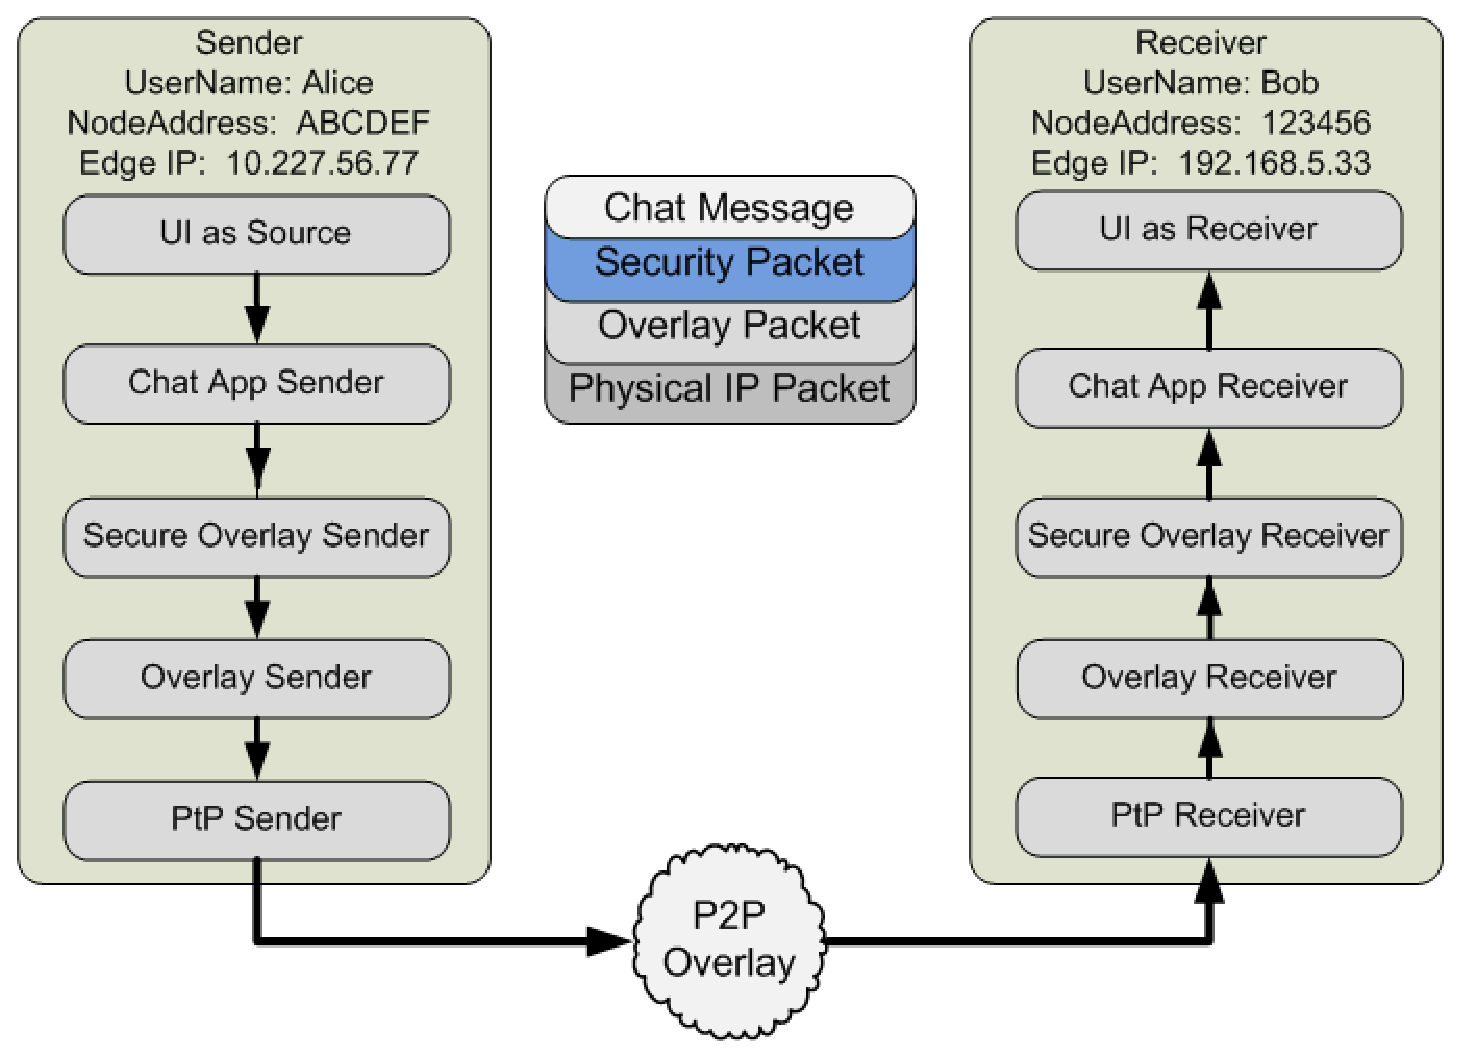
\includegraphics[width=4in]{secure_sender_stack_generic.png.eps}
\caption[Secure sender stack]{An example of the abstraction of senders and
receivers using a EtE secured chat application.  Each receiver and sender use
the same abstracted model and thus the chat application requires only high-level
changes, such as verifying the certificate used is Alice's and Bob's, to support
security.}
\label{fig:senders_receivers}
\end{figure}

\begin{figure}[ht]
\centering
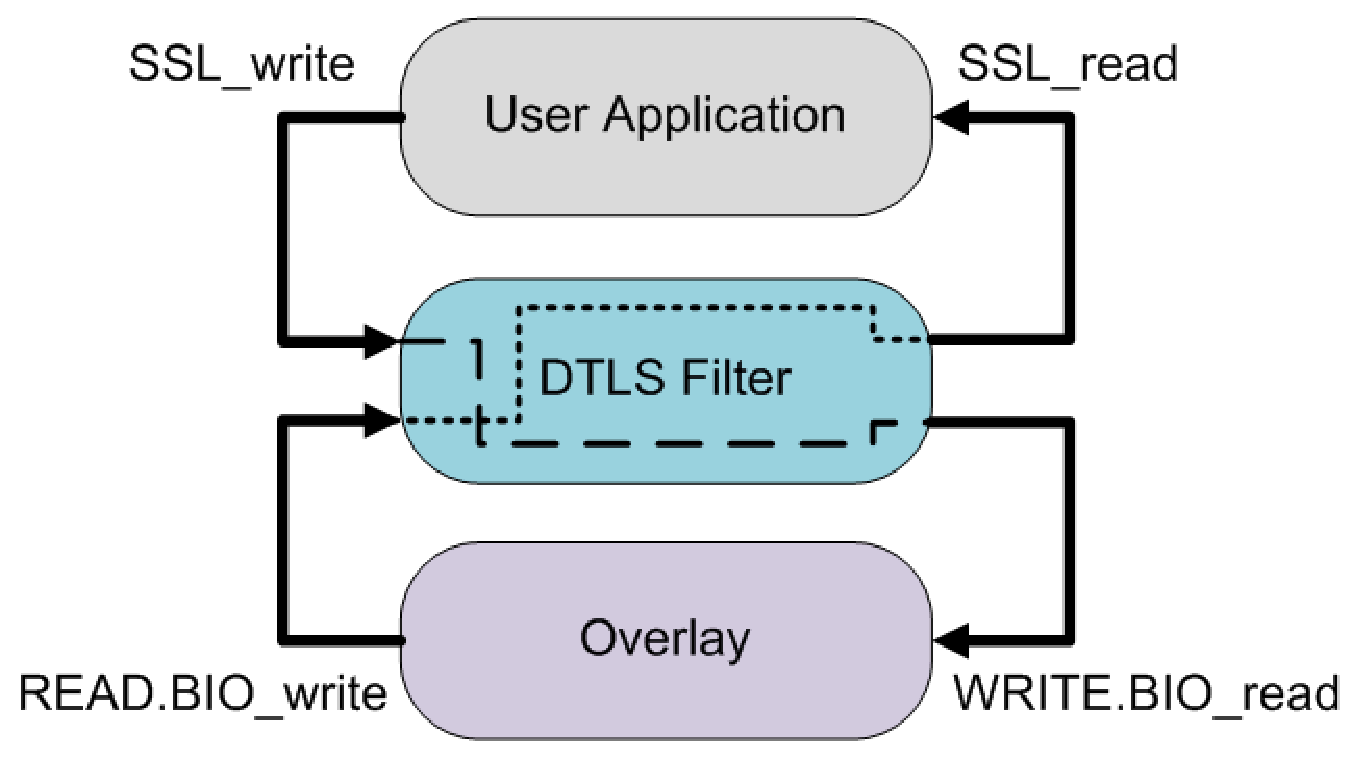
\includegraphics[width=4in]{dtls_filter.eps}
\caption[The DTLS filter.]{The DTLS Filter.  To send a secure message, execute
SSL\_write and retrieve the encrypted packet at the WRITE BIO via a BIO\_read.
To verify and decrypt a packet, execute BIO\_write on the READ BIO and retrieve
the packet via SSL\_read.  When SSL\_write or SSL\_read return the error
WANT\_READ.  This means that either it is waiting for a control message or one
is available at the WRITE BIO.  If a message is retrieved from the WRITE BIO,
it is a control message.  Because DTLS does not provide reliability when using
the memory BIO, control messages should be sent using a reliable medium, such
as a light-weight request/reply system.}
\label{fig:dtls_filter}
\end{figure}

\begin{figure}[ht]
\centering
\caption{Steps in joining a private virtual overlay.}
\label{fig:private_overlay_states}
\end{figure}

%\begin{table}[ht]
%\centering
%\begin{tabular*}{0.75\textwidth}{|l||c|c|} \hline
%& Latency (ms) & Bandwidth (Mbit/s) \\ \hline\hline
%DTLS CBC & 0 & 0 \\ \hline
%Our CBC & 0 & 0 \\ \hline
%\end{tabular*}
%\caption{CBC Issue -- In Progress.}
%\label{tab:cbc_issue}
%\end{table}

\begin{figure}[ht]
\centering
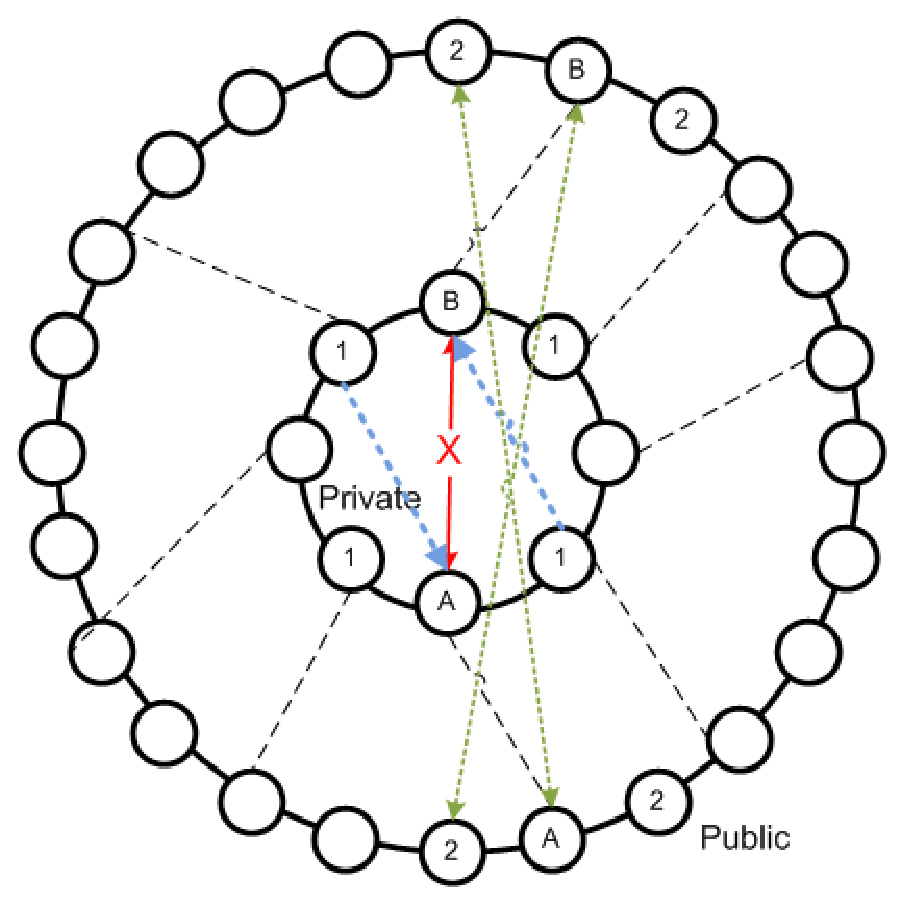
\includegraphics[width=4in]{subring_tunnel.eps}
\caption[Relays in subring environments.]{Relays in subring environments.
Creating relays across the node address space, when direct connectivity is not
possible.  Two members, A and B, desire a direct connection but are unable to
directly connect, perhaps due to NATs or firewalls.  They exchange private, 1,
and public, 2, neighbor information through the private overlay and connect to
one of each other's neighbors, creating an overlap.  The overlap then becomes a
PtP relay path (represented by directed, dashed lines), improving performance
over routing across the entire overlay.}
\label{fig:overlay_relay}
\end{figure}

\begin{figure}[ht]
\centering
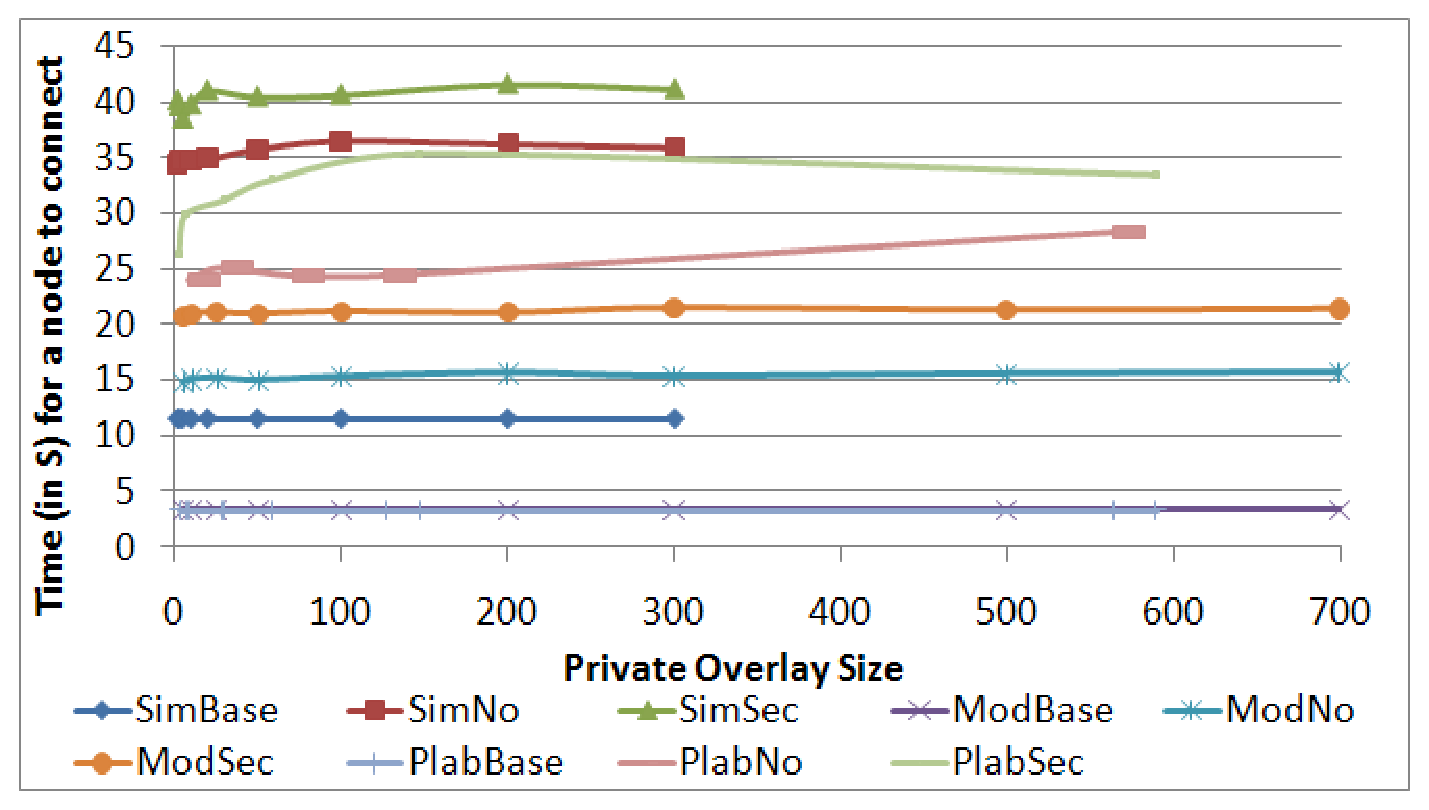
\includegraphics[width=4in]{single_join.eps}
\caption[Time taken by a single node to join public and private overlays.]{The
time it takes for a single node joining a public overlay and then a private
overlay. Since the public overlay size is the same in all tests, we averaged
all results together for the individual evaluations.  The format for the
legend is defined using the following convention: EnvironmentOverlay, where the
environment is PlanetLab, Simulator, or (Network) Modeler and overlay is Base
for public overlay, No for no security private overlay, and Sec for security
enabled private overlay. ModBase is network modeler Public overlay connection
time.  SimSec is simulator security enabled private overlay.}
\label{fig:single_join}
\end{figure}

\begin{figure}[ht]
\centering
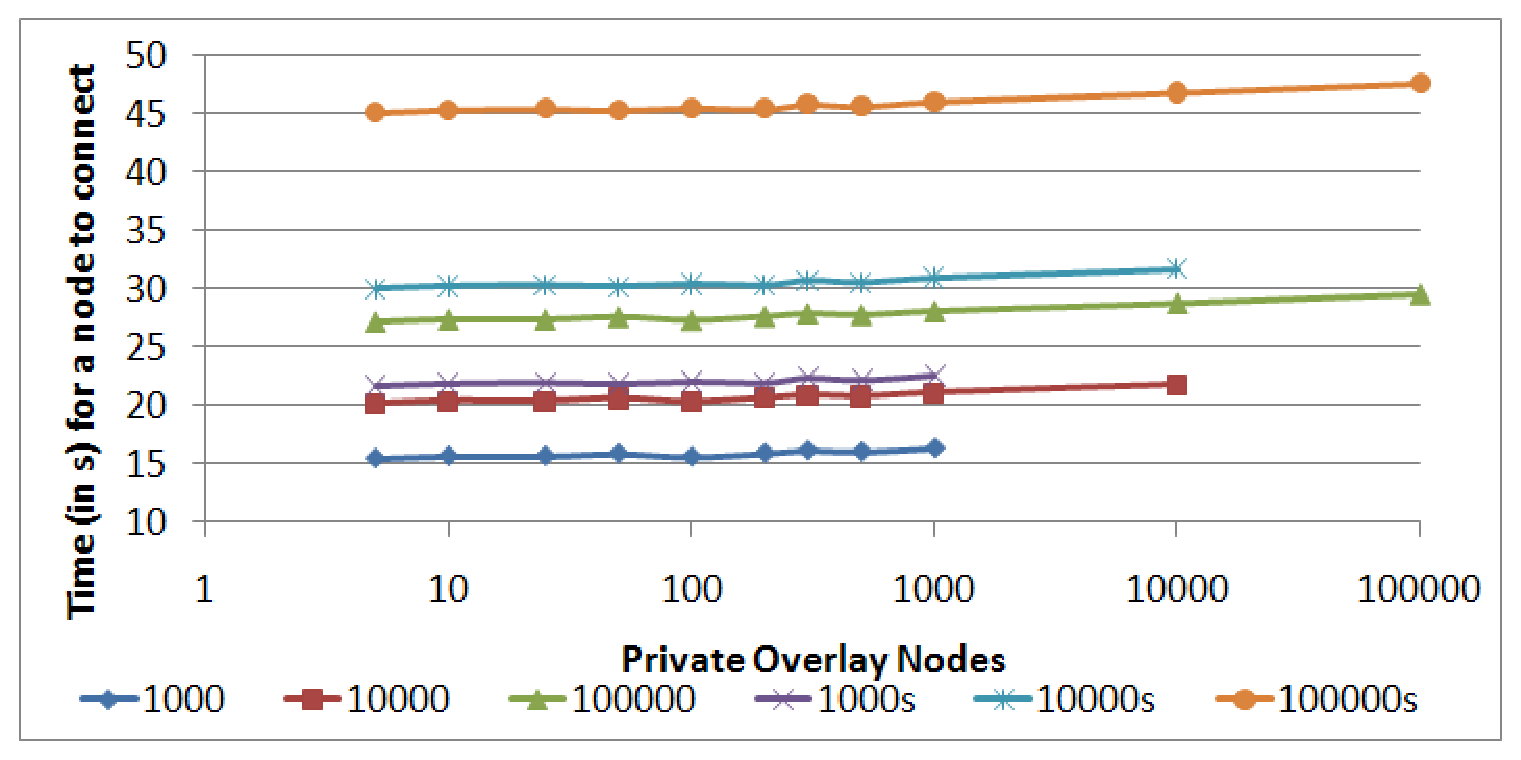
\includegraphics[width=4in]{single_join_mod.eps}
\caption[Time taken by a single node to join large public and private
overlays.]{The time it takes for a single node joining a public
overlay and then a private overlay. The X axis represents the number of peers
in the private overlay, whereas the lines themselves represent the number of
peers in the public overlay.  The legend for the line consists of
``number[s]'', where the number represents the total numbers of peers in the
public overlay and the optional ``s'' specifies whether the private overlay is
modeling security.}
\label{fig:single_join_mod}
\end{figure}

\begin{figure}[ht]
\centering
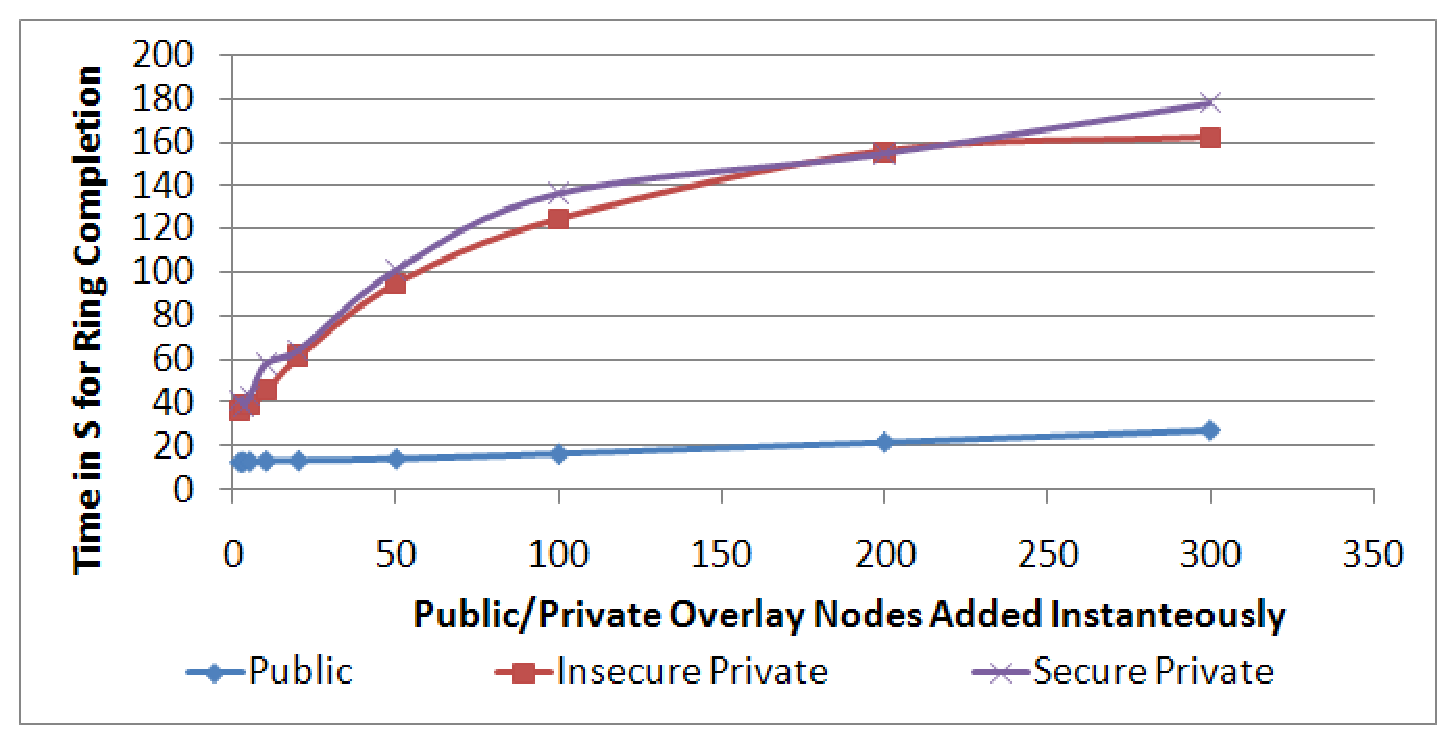
\includegraphics[width=4in]{mass_join.eps}
\caption[Large simultaneous private pool joins.]{The time to form private
overlay using a public overlay with 200 nodes after simultaneously turning on
various counts of private overlay nodes.}
\label{fig:big_join}
\end{figure}

\begin{figure}[ht]
\centering
\includegraphics[width=4in]{bandwidth.eps}
\caption[Bandwidth comparison of insecure and secure overlays.]{Bandwidth used
in a systems with and without security during steady state operations
consisting of 200 public nodes and various sized paired public / private nodes.
Those lines labeled ``static'' have DHT lists queried every 5 minutes whereas
in ``dynamic'' queries are made using an exponential back-off policy starting
at 30 seconds up to a maximum of 60 minutes.  Bandwidth is in bytes / second, a
negligible amount of bandwidth for DSL and Cable Internet.}
\label{fig:vpo_bandwidth}
\end{figure}

\begin{figure}[ht]
\centering
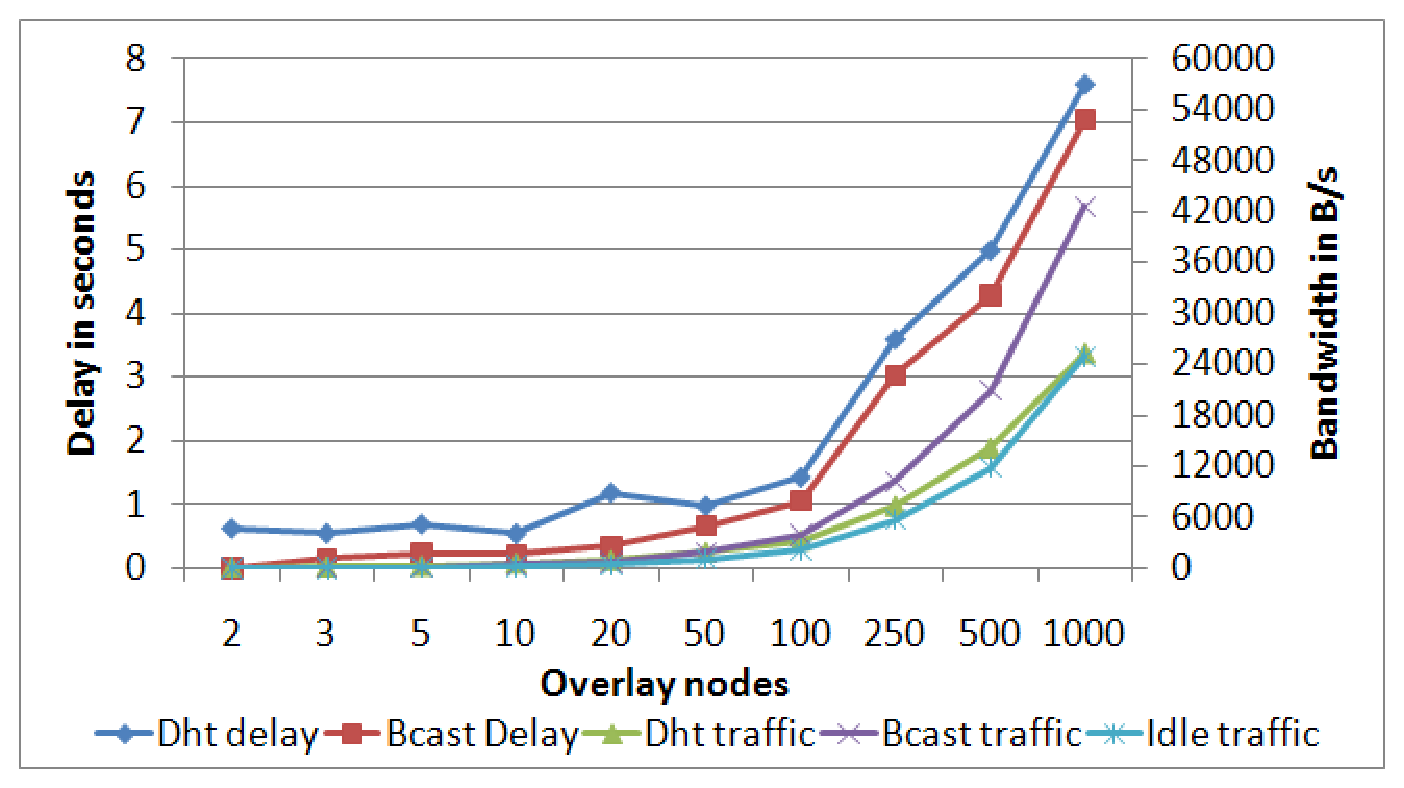
\includegraphics[width=4in]{revocation_sim.eps}
\caption[Simulated broadcast revocation evaluation.]{The time delay and
bandwidth used during the time between revoking a node and notifying nodes of
the revocation using simulations.  (Broadcast has been abbreviated to
``Bcast'').}
\label{fig:revocation_sim}
\end{figure}

\begin{figure}[ht]
\centering
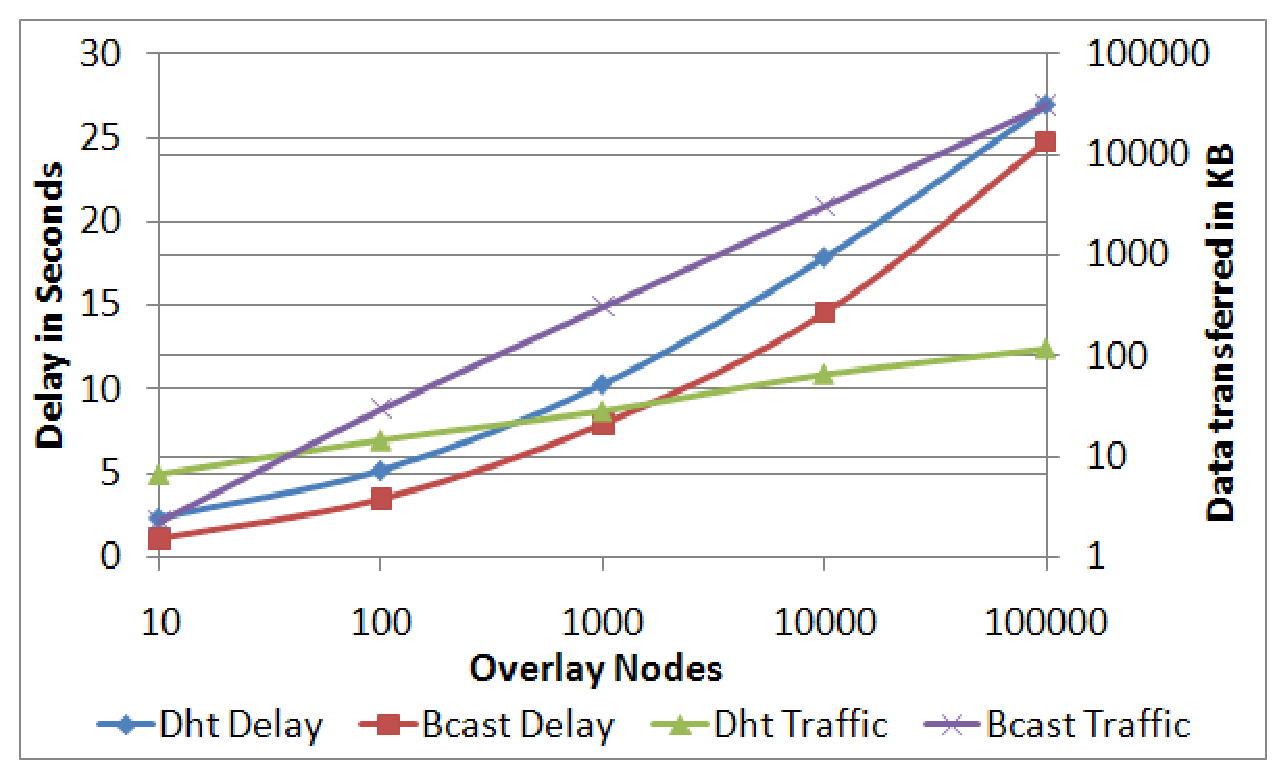
\includegraphics[width=4in]{revocation_mod.eps}
\caption[Modeled broadcast revocation evaluation.]{The time delay and bytes
transferred during the time between revoking a node and notifying nodes of the
revocation using the modeler.  (Broadcast has been abbreviated to ``Bcast'').}
\label{fig:revocation_mod}
\end{figure}


\chapter{Autonomic VPNs}
\label{vpns}
In distributed computing, there are many applications for VPNs, two such tasks
are the connecting large sets of remote resources and accessing a central
server or a personal resource.  Similar use cases can be extrapolated onto
other collaborative environments such as multiplayer games, merging home
networks over a VPN, or accessing a work computer remotely.  Each application
has different requirements and in review of related research~\cite{ipop, vine,
violin, vnet, ocala, softudc, openvpn, hamachi, wippien, gbridge, pvc, tinc,
n2n, p2pvpn, l2tp} not a single approach efficiently supports these dynamic
environments.  Certainly ISP large scale VPNs such as MPLS~\cite{mpls} do not
as well.  An overview of these and the one described in this proposal are
presented in Table~\ref{tab:virtual_networks}

The organization of a VPN has a direct effect on the amount of user effort
required to connect multiple sites.  In this regard there are two components of
a VPN, the local organization and the remote or network organization.  The setup
of the virtual network in order to have be a destination and recognized source
for remote packets consitute the local organization.  Whereas the routing of
the packets amongst peers is handled by the network organization.  Prior
research works primarily focused on the latter issue, while ignoring the former.
This meant that users were left to setup their own address allocations either
through manually configuring each environment or dealing with the head aches of
caused by DHCP servers in cross domain network construction as well as their
own security distribution systems.  In addition, organizing a network can be an
even more complicated task than locally configuring the network.  This chapter
presents a novel approach to VPNs that achieves both local and network
self-configuration.

\section{Network Configuration}
The key to communicating in a VPN is creating links to the VPN and finding
the peer in the VPN.  The different architectures for VPN link creation are
based on distributed computing communication methods and are described in
Table~\ref{tab:vpn_types}.  The approaches are described in more detail
below.

\subsection{Centralized VPN Systems}
OpenVPN is an open and well-documented platform for deploying centralized VPNs.
In this paper, it is used as the basis for understanding centralized VPNs as it
represents features common to most centralized VPNs.

In centralized VPN systems, clients forward all VPN related packets to the
server.  Client responsibilities are limited to configuring the VN device and
authenticating with the VPN server; whereas the servers are responsible for
authentication and routing between clients and providing access to the servers'
local resources and the Internet (full tunnel).  Likewise, broadcast and
multicast packets also must pass through the central server.

Centralized VPNs can support multiple servers: upon starting, the client can
randomly select from a list of known servers, implementing a simple load
balance.  Once connected, the servers provide the client an IP address in the
VPN address space. Depending on configuration this will allow a client to
communicate with other clients, resources on the server's network,
or Internet hosts via the VPN.  Servers require additional configuration to
communicate with each other.

All inter-client communication flows through a central server.  By default, a
client encrypts a packet and sends it to the server.  Upon receiving the packet,
the server decrypts it, determines where to relay it, encrypts it, and then
sends the packet to its destination.  This model allows a server to eavesdrop on
communication.  While a second layer of encryption is possible through a shared
secret, it requires out-of-band communication and increases the computing
overhead on communication.


\subsection{Centralized P2P VPN Systems}
Hamachi~\cite{hamachi} is the first well-known centralized VPN that used the
ambiguous moniker ``P2P VPN''.  In reality, these systems are better classified
as centralized VPN servers with P2P links.  Similar VPNs include
Wippien~\cite{wippien}, Gbridge~\cite{gbridge}, PVC~\cite{pvc}, and
P2PVPN\footnote{Due to the similarities between the name P2PVPN and focus of
this paper, ``P2PVPN'' refers to ~\cite{p2pvpn} and ``P2P VPN'' to to the use
of P2P in VPNs.}~\cite{p2pvpn}.  The P2P in these systems is limited to direct
connectivity between clients orchestrated through a central server: in Wippien
it is a chat server, while P2PVPN uses a BitTorrent tracker.  If NAT traversal
or firewalls prevent direct connectivity, the central server can act as a
relay.  Each approach uses their own security protocols with most using a
server to verify the authenticity and setup secure connections between clients.
In regards to the P2PVPN, long term goals involve the creation of an
unstructured, which would provide a method of decentralized organization.

\subsection{Decentralized VPN Systems}
Some examples of systems that assist in distributing load in VPN systems are
tinc~\cite{tinc}, CloudVPN~\cite{cloudvpn}, ViNe~\cite{vine}, VNET~\cite{vnet},
and Violin~\cite{violin}.  These systems are not autonomic and require explicit
specification of links between resources.  This means that, like OpenVPN, these
systems can suffer VPN outages when nodes go offline, thus administrators must
maintain the VPN connection table.  Unlike OpenVPN, these approaches typically
do not require all-to-all direct connectivity for all-to-all communication.
Users can either setup out-of-band NAT traversal or route through relays.  Links
are manually configured.

\subsection{Unstructured P2P VPN Systems}
Unlike centralized and decentralized systems, P2P environments require the
user to connect to the overlay, which then automatically configures links.
The simplest form of overlays are unstructured, where peers form random
connections with each other and use broadcast and stochastic techniques to find
information and other peers, though due to its unstructured nature, the system
cannot guarantee distance and routability between peers.  The only example of
an unstructured VPN is N2N~\cite{n2n}.  In N2N, peers first connect to a super
node and then, to find another peer, they broadcast discovery messages to the
entire overlay.  In the case that peers cannot form direct connection, peers
can route to each other over the N2N overlay.  In the realm of VPNs, all client
VPNs are also servers performing authentication though neither approach deals
with decentralized address allocation.

\subsection{Structured P2P VPN Systems}
To address the scalability concerns in unstructured systems, this work uses
structured P2P overlays.  As described in Chapter~\ref{structured_p2p},
structured P2P overlays provide distributed look up services with guaranteed
search time with a lower bound of $O(\log N)$, in contrast to unstructured
systems, which rely on global knowledge/broadcasts, or stochastic techniques
such as random walks.  In general, structured systems are able to make these
guarantees by self-organizing a structured topology, such as a 2D ring or a
hypercube, deterministically by randomly generated node identifiers.

The primary feature used by structured overlays is a distributed data store
known as a distribute hash table (DHT), which stores key, value pairs.  In
the overlay, the key is an overlay address, where the value is stored.  The
peer closest to the key's overlay address is responsible for maintaining the
value.  Cryptographic hashes like SHA and MD5 can be used to obtain the key's
overlay address from a string or some other byte array.

In~\cite{pcgrid07, i3}, a method for address allocation is described by using
the DHT.  Each VPN has a unique name or namespace, when a peer requests an
IP address, a mapping of $hash(namespace, IP)$ to the peers overlay address
is atomically written to the DHT.  A success implies that the writer was the
first writer to that value and other peers reading that value will be able to
indentify that peer as owner of that IP address in that namespace.  Likewise
when a peer wants to route a packet to a remote VPN peer, they query the DHT
using the mapping, which returns the overlay address.  The IP packet is then
sent to the overlay destination.

Unicast messages are sent between two end points on the overlay using normal
overlay routing mechanisms.  Direct overlay links can be used to improve
performance between end points.  ~\cite{ipop} describes a method by which peers
can form autonomic direct connections with each other using an unstructured
overlay.  As IP traffic increases over a period of time, a direct connection to
bypass the overlay is initiated by the receiver of the packets.  Alternatively,
a VPN may wish to form all-to-all connections with VPN peers as described
in~\cite{cops08}.

To support broadcast and multicast in an overlay, all members of a subnet
associate through the DHT by placing their overlay address at a specific key,
i.e., $namespace:broadcast$.  Then when such a packet is received, it is sent
to all addresses associated with that key.  It is up to the VN at each site to
filter the packet.  This is sufficient to support deployments where multicast
or broadcast is not relied upon extensively.  

\section{Local Configuration}
From a superficial point of view there are two approaches to local VPN
configuration a single VN endpoint per a host (Interface) and a VN router
endpoint for many hosts on the same LAN (Router).  The components differing
between the two approaches are:
\begin{itemize}
\item \textbf{Software location} - Interfaces execute the software on each VPN
connected resource, whereas any machine connected to the same LAN as a Router
will be able to access the VPN.  The Router requires a dedicated resource.
\item \textbf{Network configuration} - Since the Interface software runs on
each machine, it is able to directly configure networking parameters, whereas a
Router must use external methods to configure the resources.
\item \textbf{Communication on a LAN} - When two peers on a LAN using a VPN
Interface to communicate, all traffic must pass through the VPN adding
unnecessary overhead, though in a Router the two peers have a merged physical
and virtual network between them and the traffic is able to bypass the VPN.
\item \textbf{Fault tolerance} - The Router only has a single instance running,
when it goes offline, all resources will lose their VPN access, whereas each
individual resource has their own Interface and is responsible for their own
VPN connectivity.
\item \textbf{Communication over the WAN} - Performing encryption can be
expensive and may limit the bandwidth available due to CPU constraints.  A
Router may struggle to use all the available bandwidth, whereas enough
Interfaces will eventually be able to use all the bandwidth.  Although each
additional VPN Interface also has idle traffic, potentially reducing usable
bandwidth.
\end{itemize}

This proposal identifies methods by which a single software stack can be
implemented to support self-configuration and resource migration in a way that
is platform independent.  This method lends itself to a new architecture known
as Hybrid, allowing an instance to be run on each VPN resource but enabling
direct communication amongst peers on a LAN as described in~\cite{sc09}.  The
architectures are shown communicating via an overlay in
Figure~\ref{fig:three_models} and compared in Table~\ref{tab:three_models}.
The two aspects that need configuration in the local configuration beyond the
VPN architecture are address allocation, obtaining and setting an IP address on
a resource, and address resolution, determining where to route a VPN packet.
The keys to creating this environment involve the use of standard network
protocols implemented uniformly across operating systems, including DHCP
(dynamic host configuration protocol) and ARP (address resolution protocol).
Many applications make use of names instead of IP addresses to resolve peers,
as such a naming system, like DNS (domain name service) is almost as important
as address resolution and allocation.  A state machine representation of this
architecture is shown in
Figure~\ref{fig:vn}.

\subsection{Local VPN Architecture}
As described in the introduction, the TAP device is the glue by which the local
resources communicate with the VPN.  Each approach relies on the TAP device
though in different configurations.  In the Interface
(Figure~\ref{fig:interface}), the TAP device is used directly by the user as
any other network device.  In short, packets are written to the TAP device by
the O/S sockets and read by the VPN software to send to the remote location,
packets received by the VPN are written to the TAP device and delivered to
sockets by the O/S.  The Router (Figure~\ref{fig:router}) bridges the TAP
device to a LAN, thus packets can be routed to it and sent through the VPN.
TAP device virtualizes a bridge to other physical networks.  

Finally, the Hybrid (Figure~\ref{fig:hybrid}) like the Router connects to the
LAN but only allows configuration from the local host.  In Linux this is
possible through the use of a VETH pseudo device that provides a virtual
Ethernet pair, so that one end can be bridged with the TAP device and LAN while
the other provides another interface that can be configured on the LAN, which
will be used by the VPN.  The reason for this lies in the nature of the state
of the interfaces connected to the bridge, which go into promiscuous mode, so
that all packets sent to them are forwarded on as if they are on a wire as if
there were only a single network interface.  In non-promiscuous mode, the
network card will drop packets that are not destined for that network card.
So in that case, it is not possible to assign more than one IP address to a
bridge, because it and all devices connected to it are viewed as one big network
interface.  Connecting the VETH device allows an additional uniquely
identifiable Ethernet addresses and thus additional IP addresses.  In contrast,
aliasing a Ethernet card only provide additional IP addresses and services that
rely on layer 2 networking. In this case, some services may not work, for
example, DHCP does not work on aliased network cards.

\subsection{Address Resolution}
IP is a layer 3 protocol. Layer 2 devices such as switches, bridges, and hubs 
are not aware of IP addresses.  When a system wants to send a layer 3 packet
over a layer 2 network, it first uses ARP to find the layer 2 address owning
the layer 3 address.  This process, as shown in Figure~\ref{fig:arp}, begins by
the sending of a layer 2 broadcast message which contains an ARP request,
asking all members in the LAN that the node owning the target IP address
respond to the sender of the request.  If a node owns the target IP address,
it responds with an ARP reply, making themselves the sender and the original
sender is the message recipient.  The Ethernet header consists of the source
address being the sender and the target being the destination.  By listening to
these requests, layer 2 devices such as a switch can autonomously learn the
location of nodes holding Ethernet addresses are and can forward packets
through appropriate ports as opposed to broadcasting or dropping them.

In a typical IP subnet, all machines talk directly with each other through
switches.  As such, they must learn each other's Ethernet address. The VN model
used in this proposal focuses on a large, flat subnet spanning across all nodes
connected to the VPN.  To accomplish this, the VN provides the ability to
virtualize a bridge, similar to proxy ARPs~\cite{RFC0925} used to implement a
transparent subnet gateway~\cite{RFC1027}.  In this scenario, the VN would
need to respond to the ARP packets with a fake layer 2 address.  Layer 2
devices in the system would then route all packets destined for that layer 2
address to the VN.

As shown in the state machine (Figure\ref{fig:vn}), ARPs are only responded to
if (a) they are inquiring about a VN IP address, (b) the VN address is not
locally allocated, and (c) there is a P2P:IP mapping.  If all those are true,
then an ARP response is sent back to the sender.  ARPs are occasionally sent
out during the course of communication and thus if a machine migrates to a VN
router, the VN router will no longer respond with ARPs.  An ARP response sent
by the VN requires a source Ethernet address, bridges and switches will see the
response and will forward all traffic towards the TAP device for that Ethernet
address.  A VN device can use the same Ethernet address for remote entities.

Prior to the introduction of the VN hybrid, the VNs used the Ethernet address
FE:FD:00:00:00:00 to refer to remote entities.  If each VN hybrid used this
address, there would be layer 2 collision causing a single hybrid to have all
traffic sent to it.  In hybrid mode, each VN must generate a unique ``remote''
Ethernet address at run time.  Our experience and research has led us to the
following solution: (1) use FE:FD for the first two bytes as they tend to be
unallocated and (2) assign random values to the 4 remaining bytes.   Applying
the birthday problem in this context, the expected probability of address
collisions is small for typical LAN environments (less than 50\% if the average
number of VN hybrid nodes on the same L2 network is 65,000). 

The key difference from the Hybrid and Router is that the Hybrid routes for only
a single node, say ``A'', and thus msut ignore messages that do not originate
from ``A''.  The Hybrid model does not necessarily know about the existence of
all machines in a LAN, because it does not own them.  So when an ARP request
of some remote machine, say ``B'', is sent by ``A'', the Hybrid must send out
a matching request with the result being sent back to the pseudo-entity of the
transparent subnet gateway so that the VPN can determine if ``B'' exists
locally.  If no message is returned after a set amount of time (the reference
implementation used 2 seconds), then assuming that there is a peer in the
overlay with the IP address, the original ARP will be responded to with the
pseudo-entity being the target.

\subsection{Address Allocation}
IP addresses are traditionally allocated in one of three ways: 1) statically, 2)
dynamically through DHCP, or 3) through pseudo-random link-local addressing.
This model foucses on static and dynamic addressing.

The network components configurable by DHCP as defined by~\cite{dhcp0,dhcp1}
that are interesting to a VPN are addresses, routing, and other networking
related features.  While many different client and servers exist, they all tend
to support the basic features of allowing the server to specify to a client and
IP address, a gateway address, and domain name servers.  As shown in
Figure~\ref{fig:dhcp}, the steps in DHCP are:
\begin{enumerate}
\small{
\setlength{\itemsep}{0pt}
\setlength{\parskip}{0pt}
\item Client sends Discover packet requesting address.
\item Server receives the packet, allocates an address, and sends an Offer of
the address and other network configuration.
\item Client receives and acknowledges the Offer by sending a Request message
to accept the Offer.
\item Server receives Request message and returns an Ack message containing
the same details as the Offer.
}
\end{enumerate}

During the DHCP phase, the VPN communicates with a DHCP server for the VPN,
which will allocate an address for the requester.  Similarly, a VN model can
review packets coming into the VPN, review the sender IP address, and request
and notify the server of this allocation.  Treating static addresses like
DHCP enables easier configuration of the VPN, though it is difficult to handle
address conflicts.  In this model, this is done by the server ignoring the
duplicate requests, and it is up to the user to configure for a new address.
Thus DHCP provides a more reliable method in these systems.

To support scalably handle address allocation in decentralized systems, the
DHCP server is a virtual entity, parsing DHCP packets and interacting with
an overlay based DHT.  This approach does not need to be limited to structured
overlay based VPNs but can be introduced as an added value component.

An important aspect of DHCP is that after a machine has received an IP address
from the DHCP server, it always checks to ensure that the address has not been
allocated, as such the VPN should never respond to address resolutions for
local IP addressses.

If an overlay allocates an address to the VN, then the VN owns it.  The other
address that the VN owns is the null address, 0.0.0.0, which is sent during
DHCP to indicate that the machine has no address prior to the request.

\subsection{Domain Name Servers and Services}
Name services allow machines to be addressed with names that are more
meaningful to users than numeric addresses.  Certain applications and
services require domain name checking, such as Condor.  To support DNS, this
requires that the OS be programmed with the VN's DNS servers IP, typically
the lowest available IP address in a subnet.  In static configuration, this
process requires the user to manually add this address, though through DHCP
this is set automatically.

In the state representation of the VN (Figure~\ref{fig:vn}), the VN checks the
IP packet to ensure that the destination IP and port match that of the virtual
DNS server and the well-known DNS port, 53.  In the event of a match, the
packet is passed to the VN's handler for domain names.  Names are typically
used for the following purposes: 1) because applications require it, and 2) to
assist users in finding resources.  To deal with 1), the DNS can
deterministically maps IP addresses to names, such as 10.250.5.5 maps to
C250005005.  2) can be solved by using the DHT and placing key:value pairs of
the form hash(namespace:hostname) to IP address and hash(namespace:IP address)
to hostname.

\section{Supporting Migration}
There has been a rapid increase in the deployment of Virtual Machines (VMs) for
use in resource consolidation in the server industry as well as the domain of
cloud computing.  Providers of cloud computing services have adopted virtual
machines as the unit of granularity for providing services and service level
agreement to the users.  Users are billed according to the number of VMs and
their uptime. Major cloud-computing providers including Amazon EC2 and Go-Grid
have adopted Xen as the virtualization platform for their services and sell
compute resources in the form of virtual machines.

Apart from advantages like performance isolation, security, and portability, one
of the significant advantages of using VMs is the capability to migrate the VM
with its entire software stack from one physical host to another.  This
migration may be performed in a stop-restart manner, where the VM is paused,
migrated to another host and restarted, or in a live mode, which attempts to
minimize down time to reduce interruption of services running on the VM.

VMs including Xen~\cite{xen-live}, VMware ESX~\cite{vmotion} and KVM~\cite{kvm}
support migration with two critical requirements: (1) file systems (disk images)
must be on a shared storage system (i.e. network file systems or storage area
networks) and (2) to maintain network connectivity, the migration must occur
within an IP subnet.  In order to retain network connectivity after migration,
the VMM must notify the LAN of the VM's new location.  The new VMM host
generates an unsolicited ARP reply which broadcasts to the entire network the
VM's new location.  

The VN Interface and Hybrid models support migration of the virtual address
using techniques previously described in~\cite{ipop}.  This is a product of the
decentralized, isolated overlay approach where each overlay end point has a
one-to-one mapping to VN end point, e.g., P2P to IP.  When a VN Interface or
Hybrid model migrates, the overlay software must reconnect to the overlay, at
which point, packets will begin to be routed to the VN endpoint again,
completing migration.

Unlike Interface and Hybrid models, the VN Router does not support a one-to-one
mapping.  In fact, a VN router tends to have one P2P address for many IP
addresses.  When a machine with a VN IP wants to migrate, it cannot also take
its P2P address with it otherwise it would end connectivity for the rest of the
members of the VN router shared  overlay end point.  A solution to this
problems requires the ability to delete IP-to-P2P mappings in the DHT, detect
new addresses on the network, and inform senders that an IP is
no longer located at that overlay end point.  With these capabilities,
transparent migration can be achieved for the VN router model as follows. 

The VMM initiates a migration on a source node. Until the migration completes,
the VN router at the source continues to route virtual IP packets for the
VM. Upon completion of migration, the VN router at the target learns about
the presence of the migrated VM by either receipt of an unsolicited ARP
or by proactively issuing periodic broadcast ICMP messages on its LAN.
The VN router attempts to store (Put) the IP:P2P address mapping in the DHT,
and queries for the existence of other IP:P2P mapping(s). If no previous
mappings are found, the VN router assumes responsibility for the IP
address. Otherwise, the VN router sends a migration request to each P2P
address returned by the DHT. The VN router receiving a migration request
confirms the existence of the IP address in its routing table and that if
there is that there is no response to ARP requests sent to the IP address.
If these conditions hold, it deletes its IP:P2P mapping from the DHT and returns
true to the migration request; otherwise, it returns false. If the migration
request returns true, the VN router at the target LAN starts routing for the
virtual IP address; if it returns, false, the VN router does not route
for the virtual IP address until the previous IP:P2P mapping expires
from the DHT.

In addition to VN routers synchronizing ownership of the migrated virtual
IP address, any host that is connected to that machine must be informed
of the new P2P host.  Over time, this will happen naturally as ARP cache
entries expire and the IP:P2P mapping is looked up from the DHT.  Additionally,
the VN router at the source may keep forwarding rules for the migrated IP
address for a certain period of time, akin to mobile IP but not on a permanent
basis.  A more direct approach, as implemented in the prototype, involves the VN
router notifying the connected host of a change in ownership, resulting in the
host querying the DHT for the updated P2P end point.  An evaluation of tradeoffs
in the migration design, while interesting, is outside the scope of this paper. 

A static address allocation is similar to a migration without there being an
IP:P2P value in the DHT, though without querying the DHT, the situation is
unclear.  Systems that use DHCP only must have some method for detecting new
addresses, because there is no guarantee that a DHCP will occur immediately
following migration, in fact, depending on the lease time that is highly
unlikely.  Using an insecure DHT that supports deletes is sketchy as it would
be relatively easy for machines to perform man in the middle attacks by
deleting keys which they do not own.  Even the use of passwords mentioned in
DHT literatures is not sufficient as it is not immune to collusion, or Sybil,
attacks.

VN router migration was analyzed through the use of two Xen-based VMware VMs
co-located on the same quad-core Xeon 5335 2 GHz machine each with 1 GB memory
allocated using a minimally configured OS with a SSH server.  The evaluation
attempts to understand overlay overheads of the approach.  The experiment, as
shown in Figure~\ref{fig:migration_ring}, involved migrating a Xen guest VM
between two Xen host VMMs running in VMware.  Although they are hosted in the
same infrastructure, the two domains are connected to two separate VLANs, and
thus isolated.  The reosurce information is stored in a DHT running on top of
PlanetLab.  Thus the migration overheads in the experiment capture the cost of
wide-area messaging in a realistic environment.  During the course of the
experiment, over 50 different IP addresses were migrated 10 times each in an
attempt to gain some insights in the cost of using the DHT with support for
deletes and VN router messages as a means to implement migration.  The result,
presented in Figure~\ref{fig:mig} gathered from the experiment was how long the
VN IP was offline, measured by means of ICMP ping packets.  On average, the
overhead of VN migration was 20 seconds. This overhead is in addition to the
time taken to migrate a VM, since the VN routers begin to communicate only
after migration finishes. 

\section{Enhancing the Structured P2P VN with Private Virtual Overlays}
The use of group enabled private virtual overlays enable two qualities for
VPN:  user-friendly security and more efficient methods for broadcast and
multicast IP communication.

\subsection{Securing the VPN Through Groups}
\label{groupvpn}
The premise for secure a structured overlay VPN extends from the work on
group enabled private virtual overlays.  Each VPN will use a unique private
overlay secured by a group-enabled PKI.  For VPN purposes, both the overlay
control messages are encrypted as well as IP traffic, protecting the overlay
from malicious third-parties but all the IP traffic between two members from
other members.

The group overlay model requires a few modifications to be applied to a group
VPN.  During the creation of the group, the administrator configures the VPNs
address range, namespace, enabling security, and if they would like to use an
existing public overlay network or provide their own set of overlay nodes.
When a user has been accepted into the group, they are able to download VPN
configuration data, which is used to self-configure the VPN.  The configuration
is self-contained and requires that the user provide it to the VPN, by either
placing it in a specific directory, a GUI, or a command-line utility whose only
input parameter is the path to a configuration file.  In the prototype, the
only the file system and command-line approaches have been implemented.  The
configuration data contains the IP address space, VPN namespace, group website's
address, and a shared secret.  The shared secret uniquely identifies the user,
so that the website can determine how to handle certificate requests.  When
making a certificate request, the user sends over HTTPS a public key and their
shared secret, the website creates and signs a certificate request based upon
the public key and the user's relevant information ensuring that users cannot
trick the website into signing malicious data.  Upon receiving the signed
certificate, peers are able to join the private overlay and VPN enabling
secure communication amongst the VPN peers.

\subsection{Broadcasting IP Broadcast and Multicast Packets Via the Overlay}
The use of a private virtual overlay enables a new method for sending multicast
and broadcast packets. Approaches such as broadcasting to the entire overlay
are not suitable because the overlay could consist of peers from other VPNs and
those not even involved with VPN operations, while approaches that generate
unicast messages when a broadcast or multicast packet arrives at the VPN (e.g.
by querying a DHT key where all peers in the VPN would place their overlay
address so that they could receive the packets) do not scale well. The
abstraction of a private virtual overlay enables scalable broadcasting within a
VPN because the only peers in the private overlay are peers for a single VPN.
The broadcast method used is described in Appendix~\ref{broadcast} to
efficiently distribute messages.  Though in VPN situations, many peers may
already have connections to most if not all of their VPN peers, thus the
broadcast algorithm has been modified to route to only connections created for
structured overlay purposes and not explicitly only for VPN purposes.
Otherwise in many cases, this algorithm will degenerate into one similar to
the previous approach.  

A validation of the overlay broadcast method for IP broadcast and multicast
communication comparing it to the original DHT method is presented in
Figure~\ref{fig:broadcast}.  Metrics measured include bandwidth used by
the packet originator and time required for all peers to receive the packet.
System bandwidth remains the same as bounded-broadcast requires exactly N
messages to broadcast the message to the entire overlay.  By using a broadcast
algorithm to route multicast and broadcast IP packets instead of the unicast
packets, the sending node has much less used bandwidth.  The time required by
the DHT approach involves the time to retrieve all entries from the DHT and the
latency to the peer farthest away.  Whereas the broadcast approach has no DHT
lookup and is somewhere around the average latency in the system multiplied by
$O(\log^2 N)$.

\section{Full Tunnel VPN Operations}
\label{full_tunnel}
The configuration detailed so far describes a split tunnel: a VPN connection
that handles \emph{internal VPN traffic only, not Internet traffic}.  Prior
to this work, only centralized VPNs currently support full tunnel: providing
the features of a split tunnel in addition to securely forwarding
\emph{all their Internet traffic} through a VPN gateway.  A full tunnel provides
network-layer privacy when a user is in a remote, insecure location such as an
open wireless network at a coffee shop by securely relaying all Internet traffic
through a trusted third party, the VPN gateway.  Both models are illustrated
in Figure~\ref{fig:tunnel}.

Central VPN clients use full tunneling through a routing rule swap, setting
the default gateway to be an endpoint in the VPN subnet and traffic for the
VPN server is routed explicitly to the LAN gateway.  This rule swap causes
all Internet packets to be routed to the VN device and the VPN software
can then send them to the remote VPN gateway.  At the VPN gateway, the packet
is decrypted and delivered to the Internet.  A P2P system encounters two
challenges in supporting full tunnels:  1) P2P traffic must not be routed
to the VPN gateway and 2) there may be more than one VPN gateway.  We address
these issues and provide a solution to this problem in Section~\ref{full_tunnel}.

The challenges faced in a decentralized P2P VPN are providing decentralized
discovery of a VPN gateway and supporting full tunnel mode in a P2P environment
such that all P2P traffic is sent to the intended receiver directly instead of
through the gateway.  The remainder of this section covers gateway and
client solutions to address these challenges.

\subsection{The Gateway}
\label{the_gateway}
A gateway can be configured through NAT software, like masquerading in IPtables
or Internet Connection Sharing with Windows.  This automatically handles the
forwarding of packets received on the NAT interface to another interface
bringing the packet closer to its destination.  Similarly, incoming packets
on the outgoing interface must be parsed in order to determine the destination
NAT client.

Following from the original design of the VPN state machine in
Figure~\ref{fig:vn}, if a VPN is a gateway, the VPN state machine no longer
rejects packets, when the destination is not in the VPN subnet, though when the
VPN gateway mode is disabled these packets are still rejected.  When enabled,
all Internet and non-VPN based traffic is written to the TAP device setting the
destination Ethernet address to the TAP device.  The remaining configuration is
identical to other members of the system as packets from the Internet will
automatically have the clients IP as the destination as a product of the NAT.
To provide for dynamic, self-configuring systems, VPN gateways announce their
availability via an entry in the DHT.  As future work, this approach can be
explored to provide intelligent selection and load balancing of gateways.

\subsection{The Client}
VPN Clients wishing to use full tunnel must redirect their default traffic to
their VN device.  In the protoype VPN model, a virtual IP address is allocated
for the purpose of providing distributed VN services DHCP and DNS.  This same
address is used as the the default gateway's IP.  Because this IP address never
appears in a Internet bound packet, only its Ethernet address does, as shown in
Figure~\ref{fig:tunnel_packet}, this approach enables the use of any and
multiple remote gateways.

To support full tunnel mode, the VPN's state machine has to be slightly modified
to handle outgoing packets destined for IP addresses outside of the VPN, only
rejecting them when full tunnel client mode is disabled.  When enabled, the VPN
software sends packets to the remote peer acting as a full tunnel gateway.
Likewise, incoming packets that have a source address outside the subnet should
not be rejected but instead the overlay address should be a certified VPN
gateway prior to forwarding the packet.

To select a remote gateway, peers query the DHT.  As there may be multiple
gateways in the system, the peer randomly selects one, forwarding packets to
that node.  To ensure reliability, when the client has not heard from the
gateway recently, the client sends a liveness query to the gateway.  If the
gateway is down, the taken pessimistic approach finds a new gateway when
the next Internet packet arrives.

The real challenge in applying full tunnel VPN mode to P2P VPNs is the nature
of the P2P system, namely dynamic connections.  Peers do not know ahead of time
what remote peer connections will be thus a simple rule switch does not work.
Our original thought was to watch incoming connection requests and adding
additional routing rules on demand, though this is only reasonably feasible
with UDP as a TCP handshake message would need to be intercepted and potentially
replayed by the local host in order to enable the rule and allow proper routing.
The real drawback of the approach though is that UDP messages can easily be
spoofed by remote peers enabling unsecured Internet packets to be leaked in the
public environment.  Even if the connections are secured, it could take some
time for the peers to recognize a false connection attempt and delete the rule.

A solution to the security problem is to have all traffic directly routed to
the VN device with no additional routing rules.  The VN is then responsible for
filtering P2P traffic and forwarding it to the LAN's gateway via Ethernet
packets.  In the VPN application, outgoing IP packets' source ports are
compared to VPN application's source ports.  Upon a match, the VPN application
directs the packet to the LAN's gateway.  The three steps involved in this
process are 1) translating the source IP address to match the physical
Ethernet's IP address, 2) encapsulating the IP packet in an Ethernet packet
with a randomly source address~\cite{sc09} and the destination the LAN's
gateway, and 3) sending the packet via the physical Ethernet device.  Sending
an Ethernet packet is not trivial as Windows lacks support for this operation
and most Unix systems require administrator privilege.  Our platform
independent solution uses a second TAP device bridged to the physical Ethernet
device, allowing Ethernet packets to be sent indirectly through the Ethernet
device via the TAP device.  Because the solution results in incoming packets to
arrive at a different IP address than the actual original source IP address TCP
does not work in this solution.  This method has been verified to work on both
Linux and Windows using OS dependent TAP devices and bridge utilities.

\subsection{Full Tunnel Overhead}
\label{full_tunnel_eval}
While the full tunnel client method effectively resolves the lingering problem
of ensuring that all packets in a full tunnel will be secure, it raises an
issue:  could the effect of having all packets traverse the VPN application be
prohibitively expensive.  Analysis of this approach compares it with one that
uses the traditional routing rule switch.  Figure~\ref{tab:full_tunnel_eval}
present the ping time from a residential location to one of Google's IP
addresses using a gateway located at the University of Florida when the VPN is
in split tunnel mode, full tunnel using the routing rule switch, and full
tunnel using Ethernet forwarding.  The results express that there is negligible
difference between the full tunnel approaches.  One interesting result is the
latency to gateways public address in the routing test, which most likely is a
result of the ping being sent insecurely avoiding the VPN stack completely.

\section{Evaluation of VPN Network Configuration}
This experiments explores bandwidth and latency in a distributed VPN system to
motivate the usage of P2P links in a VPN.  The VPNs used are include the
prototype (IPOP), OpenVPN, and Hamachi.  OpenVPN represents a typical
centralized VPN, while Hamachi represents a well-tuned P2P-link VPN.  The
evaluation was performed on Amazon EC2 using small instance sized
Ubuntu i386 instances to create various sized networks ranging from 1 to 32.
OpenVPN uses an additional node as the central server and Hamachi has an upper
bound of 16 due to limitations in the Linux version at the time of this
evaluation.  To perform bandwidth tests, the instances are booted and query an
NFS for the list virtual IP addresses, peers are ordered such that half the
peers are act as clients and the other half the peers creating a 1 to 1 mapping
between all sets.  Latency and bandwidth tests are performed using netperf's
request-reply and streaming tests respectively.  Prior to the start of the
tests, peers have no knowledge of each other, except the virtual IP addresses,
thus connection startup costs are included in the test.  Test are run for 10
minutes diluting the connection initiation overhead but represent an example of
real usage.  Results from the clients are polled at all locations and averaged
together, though the OpenVPN server is measured separately.  IPOP and OpenVPN
use authenticated 128-bit AES, while Hamachi does not allow configuration of
the security parameters and uses the default Hamachi settings.

Figure \ref{fig:latency} and \ref{fig:bandwidth} present the results for latency
and bandwidth respectively.  Latency is measured in transactions of successful
request/reply messages.  In the latency test, it is obvious that having the
central server increases the delay between the client and server and the results
degrade more quickly as additional peers are added to the system.  In small
systems, OpenVPN shines probably due to optimized software, though as the system
grows, the system bandwidth does not.  By the time 8 peers have entered into
the system, both decentralized approaches perform better than the OpenVPN
solution.  To summarize, decentralized VPN approaches provide better
scalability, which can be immediately noticed by low latency times and, as the
system grows, available bandwidth.

\section{Evaluation of VPN Local Configuration}
This section presents an evaluation of the different VN models, using prototype
implementations built upon IPOP.  The grid evaluation simulates a client/server
environment and investigate CPU / networking overheads related with each
approach.  In addition a cloud deployment shows a proof of concept that connects
multiple cloud and local resources as well as evaluation of overhead of the
different approaches in WAN and LAN environments.  In all WAN experiments, a
wide-area IPOP overlay network with approximately 500 overlay nodes distributed
across the world on PlanetLab resources is used to bootstrap VN connections and
to support DHT-based storage and P2P messaging.

The proposed VN models place varying demands on the resources of the systems
involved. The evaluation focuses on CPU as experience suggest that this is the
most significant limiting factor.  As will be presented, the CPU load offered
by these models depends on the bandwidth of the underlying network link, since
a larger bandwidth requires more processing of packets.  The tools for
evaluating these VN models are, Netperf and SPECjbb, described in
Appendix~\ref{evaluation_tools}.

\subsection{On the Grid}
The initial evaluation involves testing a client-server environment.  The
baseline hardware consisted of quad-core 2.3GHz 5140 Xeon with 5 GB memory and
Gigabit network connectivity.  Each VM was allocated 512 MB of RAM and ran
Debian 4.0 using a Linux 2.6.25 kernel.  The client side consisted of 4 VMs on
5 machines.  The server side consisted of 5 VMs on one machine with 4 acting
as servers and 1 acting as a gateway, which was necessary to control bandwidth
into the system, done through the Linux utility \textbf{tc}~\cite{tc}, traffic
control.  In this environment, each server had 5 clients communicating with it.
The setup is shown in Figure~\ref{fig:gridsetup}.

The evaluation results are presented in Figure~\ref{fig:gridevalnet} and
\ref{fig:gridevalcpu}.  The maximum bandwidth of 600 Mbps is achieved when
neither virtual network nor traffic shaping are enabled (``no spec.phys'' at
1000 Mbps limit in Figure~\ref{fig:gridevalnet}\subref{fig:stream.netperf}),
which is only 60\% of the theoretical maximum.  This limit is most likley the
cost of VMMs, specifically the time required for a packet to traverse both VMMs
networking stack as well as the hosts networking stack.  Another observation
was that transactions per second (Figure~\ref{fig:gridevalcpu}
\subref{fig:rr.spec}) do not improve significantly for \textbf{tc} bandwidth
limit above 25 Mbps in all cases; thus focus is on only the relevent data up to
this limit.

Distinguishing features of the different VN models include the following.
Figure~\ref{fig:gridevalnet}\subref{fig:stream.netperf} shows that bandwidth in
all VN models is comparable with traffic control limit up to 75 Mbps. Beyond
this point, the interface model achieves better bandwidth than the router model
(VN processing is distributed across multiple processes); the spec/no spec
ratio in the router model is smaller than in the interface model because there
is less resource contention caused by VN processing on end nodes. For the same
reason, the router tends to achieve better SPEC results
(Figure~\ref{fig:gridevalcpu}\subref{fig:stream.spec}) than the interface.
Figure~\ref{fig:gridevalnet}\subref{fig:rr.netperf} shows that the router
performs poorly compared to the interface model in terms of
transactions/second, though it achieves a better ratio of SPECjbb score
(Figure~\ref{fig:gridevalcpu}\subref{fig:rr.spec}) to transactions than the 
interface at constrained bandwidths (less than 5 Mbps).

The hybrid method was tested, and results were nearly identical to those of the
interface, from the point of view of the WAN part of the VN, it is the
same architecture.  These results are not reported in the plots as they
add little value and further obfuscate the results.

The bandwidth cap observed in the router approach reflects the performance
achieved by the current prototype of the router, subject to VM overheads. The
use of VM is an assumption that is valid in the domain of cloud computing
where all resources run in a VM. This experiment focused on the interplay
between resource consumption by overlay routers and application performance.
Optimized user-level overlay routers running on dedicated physical
machines have been reported to achieve performance near Gbit/s in related
work~\cite{vine2}; it is expected that the cap can be raised substantially
with improved handling of network packets and user-level router optimizations
as described in Chapter~\ref{direct_communication}.

One thing that left unevaluated that may provide more interesting data would
be providing the VN router dedicated hardware.  In the test environments, this
was infeasible, because all but one of the machines in the lab run VMware
Server 1, which has a bug with setting the virtual network card in promiscuous
mode.  This effectively makes it impossible for a VM to be a VN router as no
packets will ever make their way into the VM, as the VMM will reject all
packets.  As such, the machines hosting the servers had VMware Server 2, which
does allow setting a network interface into promiscuous mode.

\subsection{In the Clouds}
The goal of this experiment is to demonstrate the feasibility of connecting
multiple cloud providers as well as local resources together through virtual
networking.  The sites chosen for evaluation were local resources at Universty
of Florida and cloud resources provided by Amazon EC2 and GoGrid.  A
qualitative observation here was that the differences in the networking
infrastructure exposed by different cloud providers reinforce the importance
of the virtual network to allow flexibility in how end nodes are connected.
Specific network configurations for the clouds were as follows:
\begin{itemize}
\small{
\setlength{\itemsep}{0pt}
\setlength{\parskip}{0pt}
\item Amazon EC2 provides static IP networking (public and private), no
Ethernet connectivity, and no ability to reconfigure IP addresses for
network. Currently, only the VN interface model is supported.
\item GoGrid provides 3 interfaces (one public, statically configured,
and two private, which can be configured in any manner); the 2 private
interfaces are on separate VLANs supporting Ethernet connectivity. The
VN interface, router, and hybrid models are supported.
}
\end{itemize}

This experiment narrows down the performance evaluation to focus on WAN and LAN
performance of VNs in cloud environments and consider Netperf single
client-server interactions only. Amazon only supports Interface mode, thus it
is only evaluated in the WAN experiment. It has been observed that, within
Amazon, the VN is able to self-organize direct overlay connections~\cite{wow}.
Each test was run 5 times for 30 seconds, the standard deviation for all
results was less than 1.  Because of this, only the average is presented in
Table~\ref{tab:cloud-wan}.

It can be seen in Table~\ref{tab:cloud-wan} that the VN adds little
overhead in the Netperf-RR experiment. Between UF and GoGrid as well as between
UF and Amazon EC2, the overhead for the Stream experiment was about 15\%.  This
may be attributed to the additional per-packet overhead of the VN and the small
MTU set for the VN interface (1200).  The MTU, or maximum transmission unit, is
the larget packet that is sent from an interface.  IPOP conservatively limits
the VN MTU to 1200 down from the default 1500 to allow for overlay headers and
to work properly with poorly configured routers, which has encountered in
practical deployments.  A more dynamic MTU, which will improve performance, is
left as future work.  The EC2 / GoGrid experiment had greater overhead
which could possibly be attributed to by the VM encapsulation of cloud
resources.

Table~\ref{tab:cloud-lan} shows that some of the performance expectations
for the different models in a LAN were accurately predicted while others
were not so clear.  Stream results match the expectation that VN models hybrid
and router bypass virtualization and get near physical speeds, whereas interface
does not.  Interestingly, RR had rather poor results for Router and Hybrid
though further testing seems to indicate that this is an issue of using the
VLAN connected network interfaces as opposed to the public network connected
interface.

\section{Figures and Tables}

\begin{table}[ht]
\centering
\begin{tabular*}{0.75\textwidth}{|c||c|c|c|c|} \hline
& Overlay & Routing & Configuration & Miscellaneous \\ \hline\hline
IPOP
&
%Overlay
Structured P2P overlay with O(Log N) routing hops, where N is the size of P2P
network. Self-optimizing shortcuts and STUN-based NAT traversal.
&
%Routing
Mapping stored in DHT resolves virtual IP address to P2P address. Virtual
network packets are routed to corresponding P2P address.
&
%Configuration
Each machine runs P2P VPN software with a dynamic IP address in a common subnet.
Common configuration shared amongst all hosts.
&
% Misc.
Supports encrypted P2P links and end-to-end VPN tunnels (unpublished work).
Migration possible; routes self-configure without user intervention, product of
the P2P overlay.
\\ \hline
N2N
&
%Overlay
Unstructured P2P network, super nodes provide control paths, forms direct
connections for data.
&
%Routing
Broadcast for discovery and overlay for control.  No organization, no guarantees
about routing time.
&
%Configuration
Requires N2N software at each host, must connect to a super node.  Supports
layer 2 Ethernet network.
&
% Misc.
Supports shared secrets to create private tunnels between edges.  Migration not
discussed, but potentially free due to layer 2 approach.
\\ \hline
OCALA
&
%Overlay
Not tied to any specific overlay, layer 3 middleware.
&
%Routing
Based upon chosen overlay.
&
%Configuration
Requires OCALA stack, overlay configuration, and IP to overlay mapping.
&
% Misc.
Security is overlay based or SSH tunnels.  Migration not mentioned.
\\ \hline
SoftUDC VNET
&
%Overlay
Decentralized with explicitly configured overlay routes.
&
%Routing
Broadcast for discovery.
&
%Configuration
Requires software on each host and one proxy per site.  Layer 2 networking.
&
%Misc.
Security is not discussed nor is wide-area migration.
\\ \hline
ViNe
&
%Overlay
ViNe authority configures global network descriptor table (GNDT) explicitly at
each router. Supports proxying to one location through another and NAT traversal.
&
%Routing
GNDT provides overlay routes for all routers in overlay.
&
%Configuration
Each subnet is allocated a single router.  Each host must be configured for
regular and ViNe networks, but no VN software needed on host.
&
% Misc.
Supports encrypted tunnels between ViNE routers, migration not discussed.
\\ \hline
Violin
&
%Overlay
Decentralized network with statically configured overlay routes.
&
%Routing
Broadcast discovery for Ethernet, static routes for IP subnet.
&
%Configuration
Virtual hosts connect VMs to the VN.  Hosts connect to virtual switches or
proxies (gateways).  Switches connect to proxies.  Sites are typically
allocated an IP address space.
&
% Misc.
Security potentially through the use of SSH Tunnels.  Migration possible;
requires reconfiguration of switches. 
\\ \hline
Virtuoso VNET
&
%Overlay
Decentralized with explicitly configured overlay routes.
&
%Routing
Broadcast for discovery.  Bridging learns paths after initial discovery.  Virtual
network packets are routed between VNET proxies.  Can be configured manually.
&
%Configuration
Each site runs a proxy providing Ethernet bridge to other proxies.  VM hosts
forward packets to local proxy.  Proxies configured to connect to other proxies.
&
% Misc.
Security through the use of SSL and SSH Tunnels.  Layer 3 migration, product of
layer 2 virtualization.
\\ \hline
\end{tabular*}
\caption{Virtual Network Comparison}
\label{tab:virtual_networks}
\end{table}

\begin{table}[ht]
\caption{VPN Classifications}
\label{tab:vpn_types}
\begin{center}
\begin{tabular*}{0.75\textwidth}{|c|c|} \hline
Type & Description \\ \hline
Centralized & Clients communicate through one or more servers which are statically
configured \\ \hline
Centralized Servers / P2P Clients & Servers provide authentication, session management, and
optionally relay traffic; peers may communicate directly with each
other via P2P links if NAT traversal succeeds\\ \hline
Decentralized Servers and Clients & No distinction between clients and servers;
each member in the system authenticates directly with each other; links between
members must be explicitly defined \\ \hline
Unstructured P2P & No distinction between clients and servers; members either know
the entire network or use broadcast to discover routes between each other \\ \hline
Structured P2P & No distinction between clients and servers; members are usually
within $O(\log N)$ hops of each other via a greedy routing algorithm; use
distributed data store for discovery \\ \hline
\end{tabular*}
\end{center}
\end{table}

\clearpage

\begin{figure}[ht]
\centering
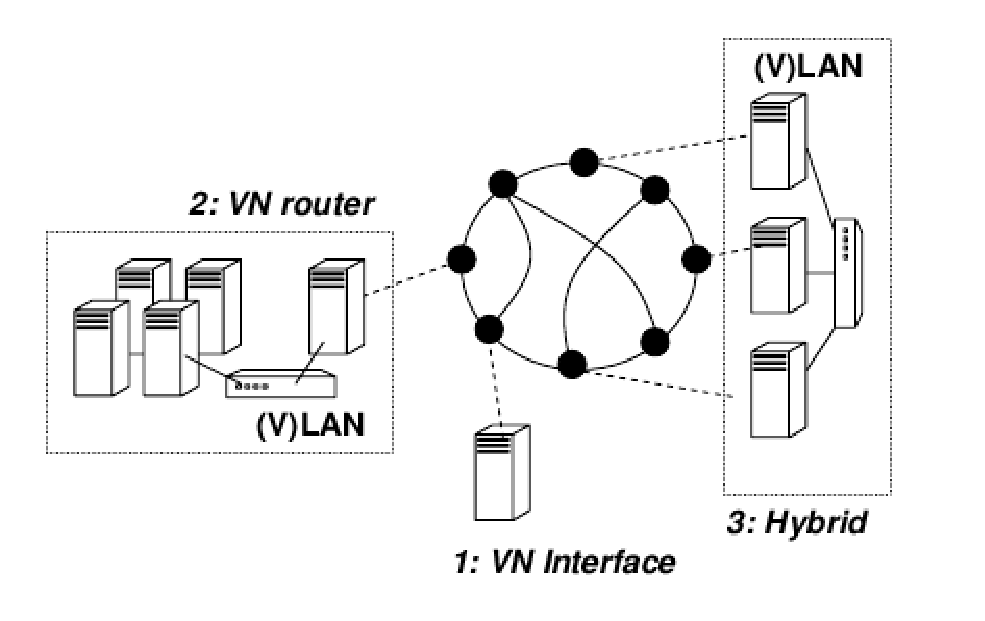
\epsfig{file=figs/three_models.png.eps}
\caption[Three VN Approaches]{Illustration of the three different deployment
models considered in this paper. In VN interface mode (1), each node has an
overlay ID and communicates to all other nodes through VN tunneling. In VN
router mode (2), only the router has an overlay ID and routes for a set of
resources; LAN communication does not require VN tunneling. In hybrid mode
(3), each host has an overlay ID; LAN communication does not require VN
tunneling.}
\label{fig:three_models}
\end{figure}

\begin{table}[ht]
\centering
\begin{tabular*}{0.75\textwidth}{|c||c|c|c|} \hline
 & Interface & Router & Hybrid \\ \hline\hline
Host LAN 
& 
No assumption 
& 
Ideally, VLAN
&
No assumption, though may have duplicate address allocation in the same subnet
for different namespaces.\footnotemark[2]
\\ \hline
Host software
&
IPOP, tap
&
End node: none. Router: IPOP, tap, bridge 
&
IPOP, tap, veth, bridge \\ \hline
Host overhead
&
CPU, memory
& 
End node: none. Router: CPU, memory
&
CPU, memory \\ \hline
LAN traffic
&
Through IPOP
&
\multicolumn{2}{c|}{Bypasses IPOP} \\ \hline
Migration
&
Handled by node
&
Involves source and target routers
&
Handled by node \\ \hline
Tolerance to faults
&
Nodes are independent
&
Router fault affects all LAN nodes
&
Nodes are independent \\ \hline
\end{tabular*}
\caption{Qualitative comparison of the three deployment models}
\label{tab:three_models}
\end{table}

\begin{figure}[ht]
\centering
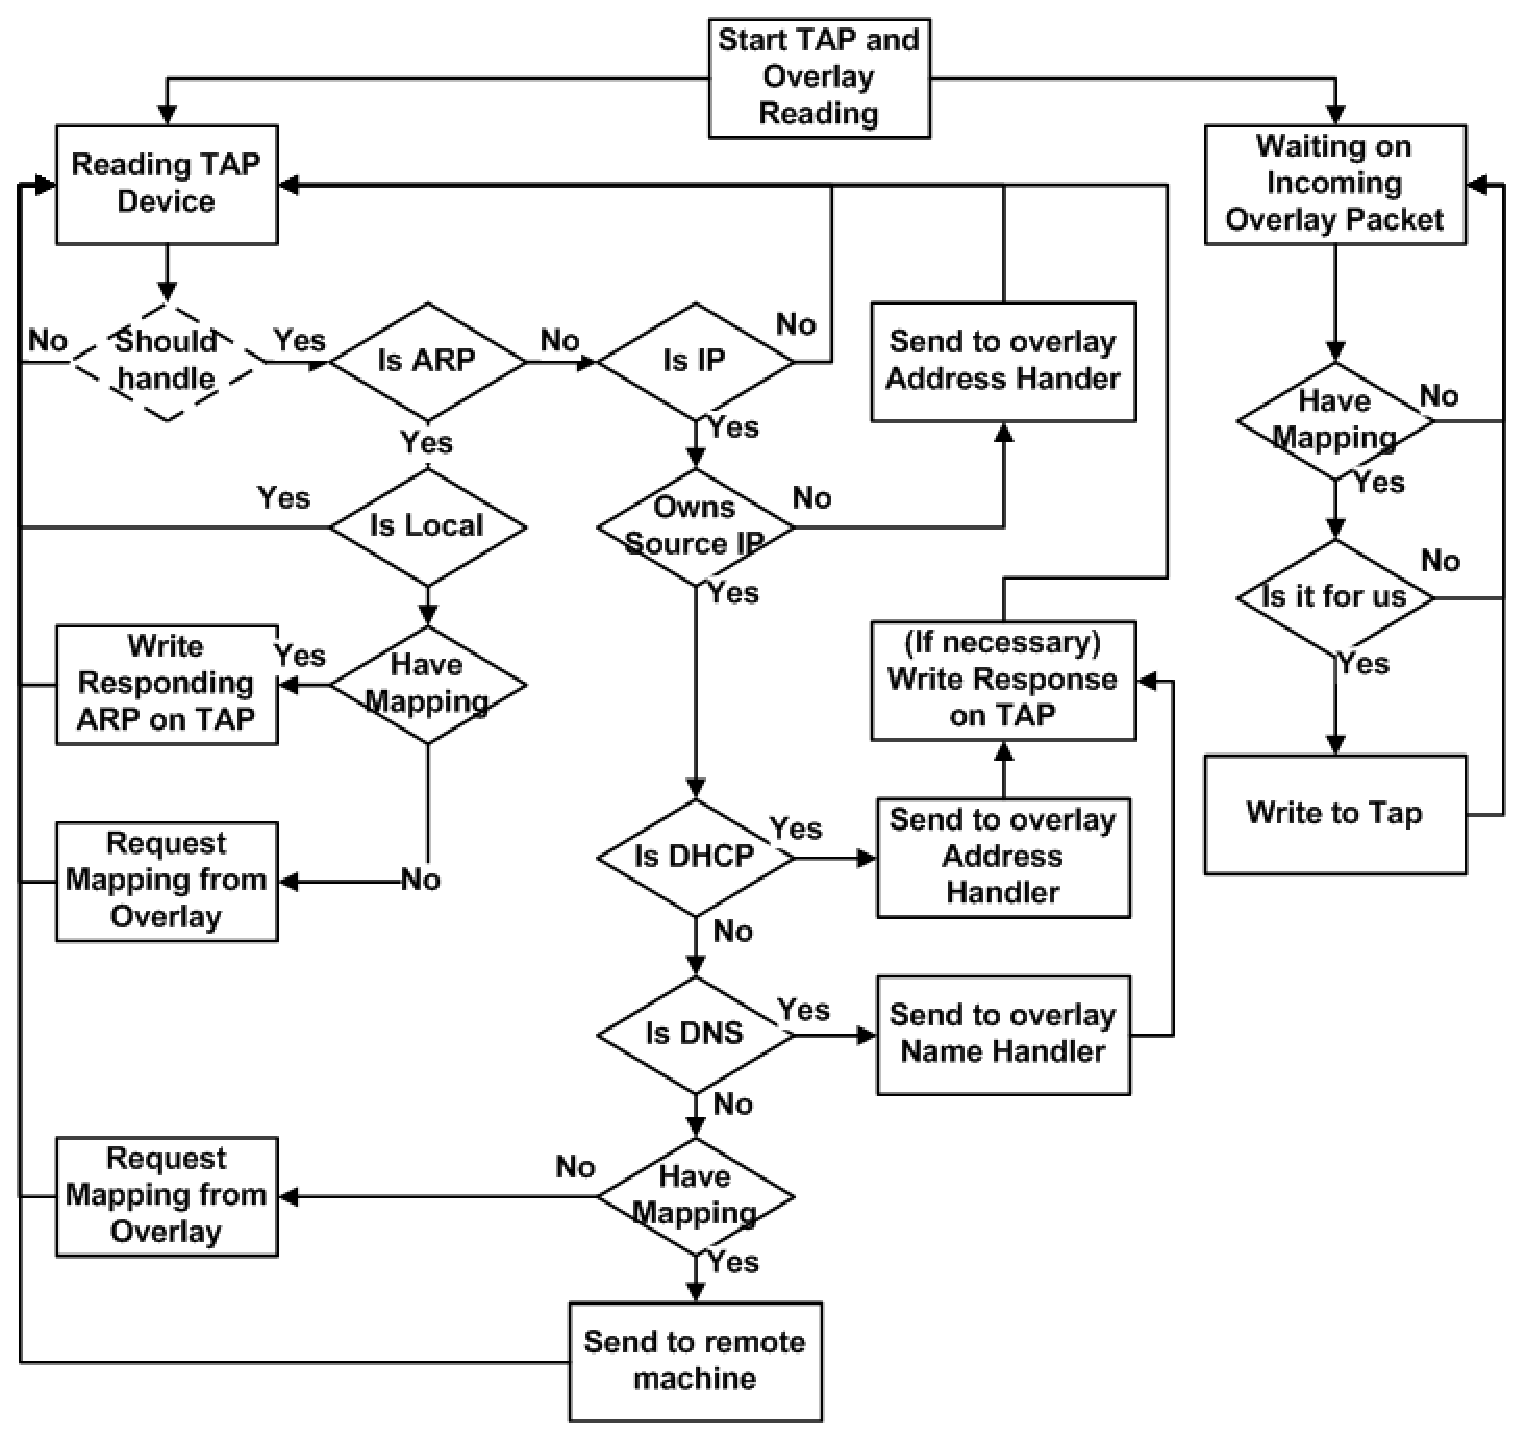
\epsfig{file=figs/vn.png.eps, width=6in}
\caption[The state diagram of a self-configuring VN.]{The state diagram of a
self-configuring VN.  In this model, a VN interface is identical to a VN router
with the caveat that the TAP device is not bridged, thus isolating the VN
traffic.  The ``Should Handle'' with dashed lines is a feature that is specific
to the VN hybrid; that is, a VN hybrid must be configured to communicate for a
single network device.}
\label{fig:vn}
\end{figure}

\begin{figure}[ht]
\centering
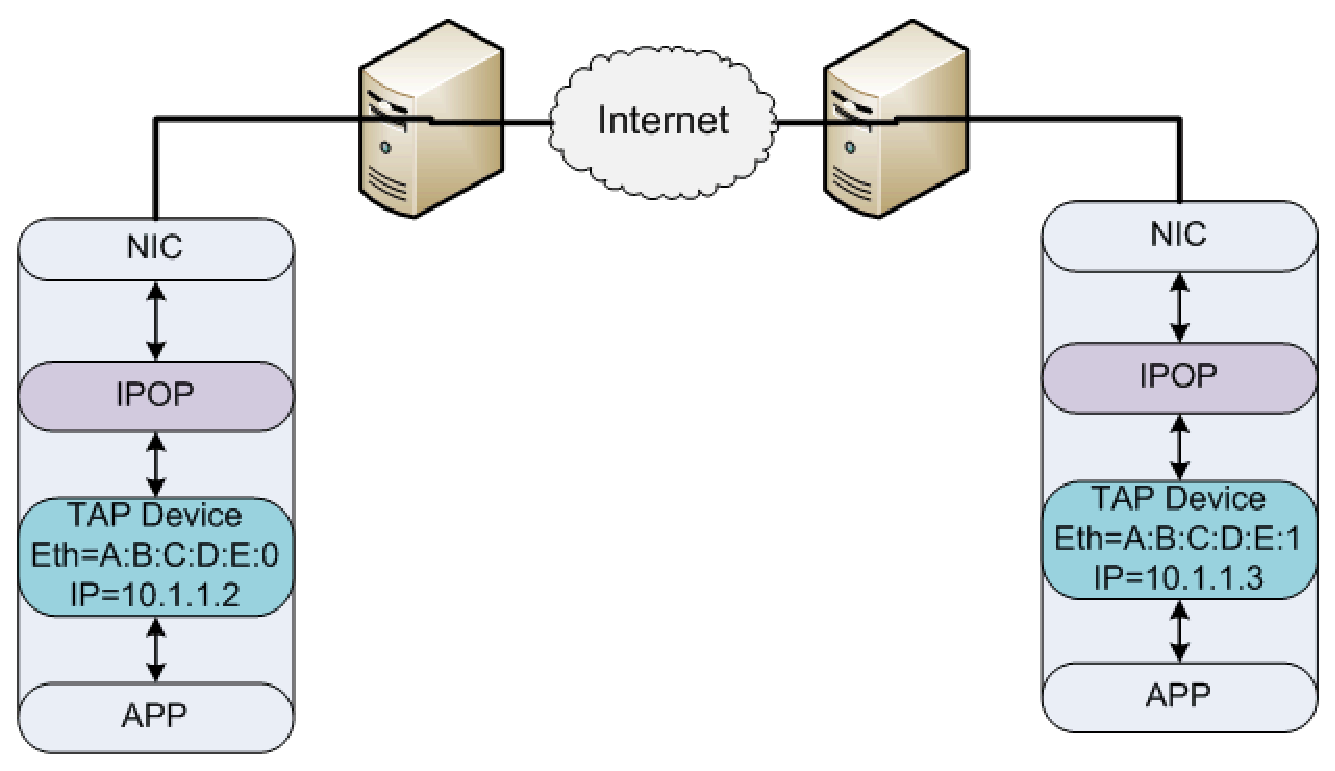
\epsfig{file=figs/tap_workstation.png.eps, width=4in}
\caption[VN Interface]{A VN deployed as an interface for single machine usage.
The user of the machine is presented two interfaces on two different IP subnets.
All non-VN subnet based traffic is routed normally via the default interface.}
\label{fig:interface}
\end{figure}

\begin{figure}[ht]
\centering
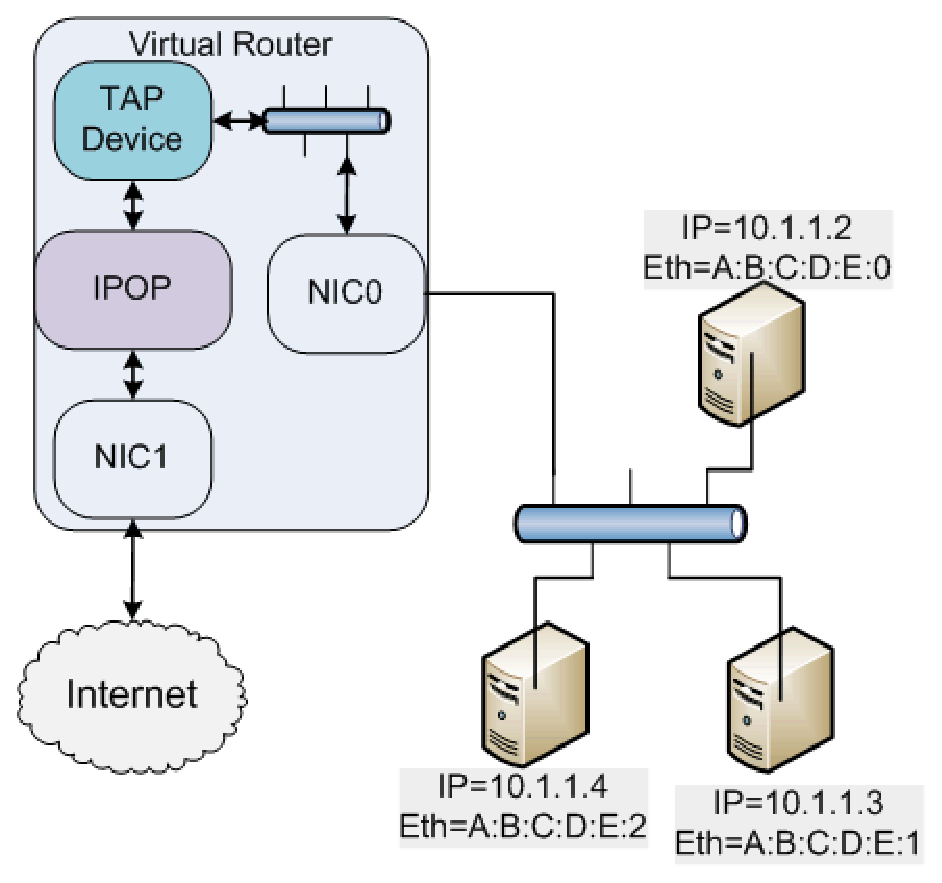
\epsfig{file=figs/tap_cluster.png.eps, width=4in}
\caption[VN Router]{A VN deployed as a router providing virtual network access
for an entire layer 2 network.  Each machine in the network only has a VN-based
address, though they can communicate directly with each other (and with proper
routing rules and NAT setup the Internet as well).  The machine hosting the VN
can also have an IP address in the network by assigning one to the bridge.}
\label{fig:router}
\end{figure}

\begin{figure}[ht]
\centering
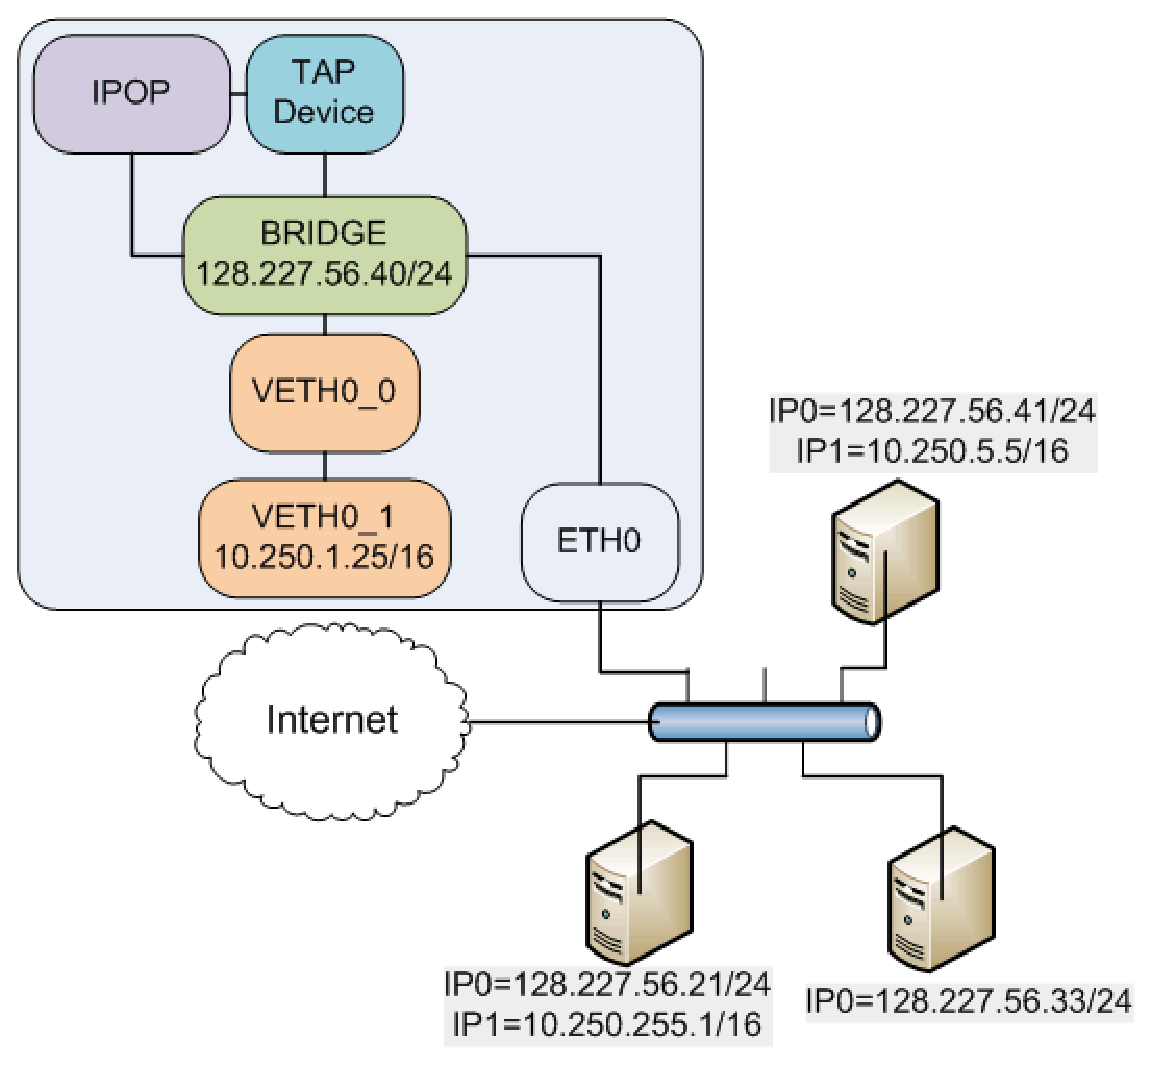
\epsfig{file=figs/tap_hybrid.png.eps, width=4in}
\caption[VN Hybrid]{A VN deployed in a hybrid mode providing virtual network
access for a single machine but bypassing the VN when a VN peer is local.  This
model is similar to having two network cards from a single machine going to one
switch.  The key feature is that this model allows a machine to be in multiple
IP address space subnets and have layer 2 traffic as well.}
\label{fig:hybrid}
\end{figure}

\begin{figure}[ht]
\centering
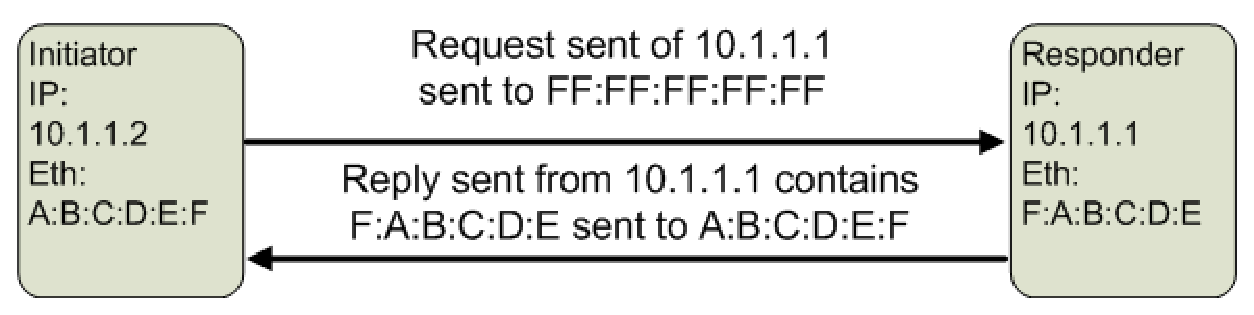
\epsfig{file=figs/arp.png.eps, width=4in}
\caption{ARP Request/Reply Interaction.}
\label{fig:arp}
\end{figure}

\begin{figure}[ht]
\centering
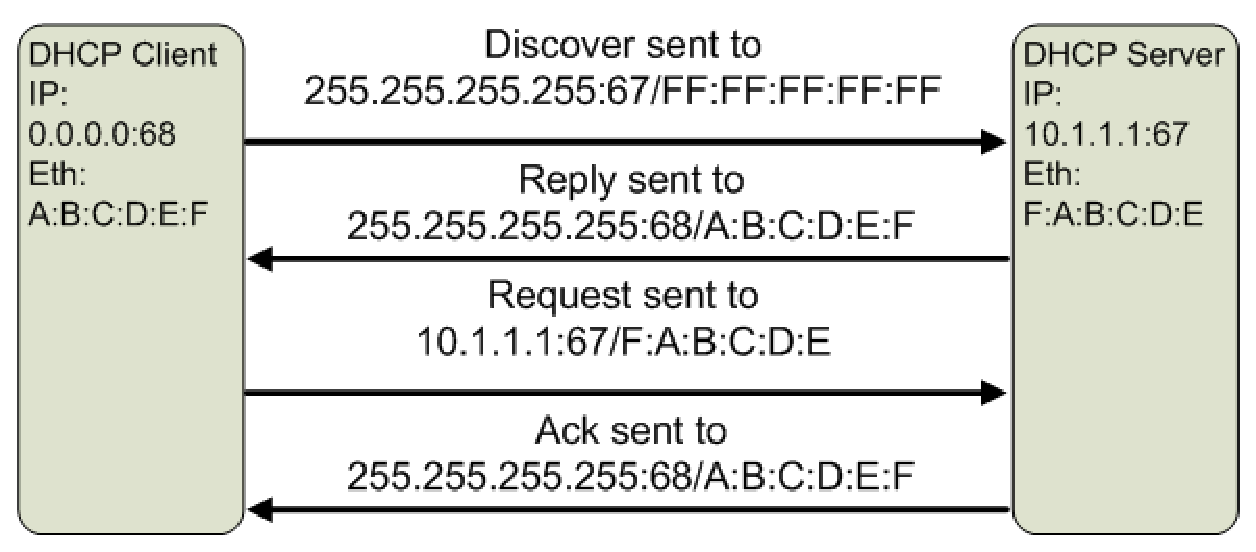
\epsfig{file=figs/dhcp.png.eps, width=4in}
\caption{DHCP Client/Server Interaction.}
\label{fig:dhcp}
\end{figure}

\begin{figure}[ht]
\centering
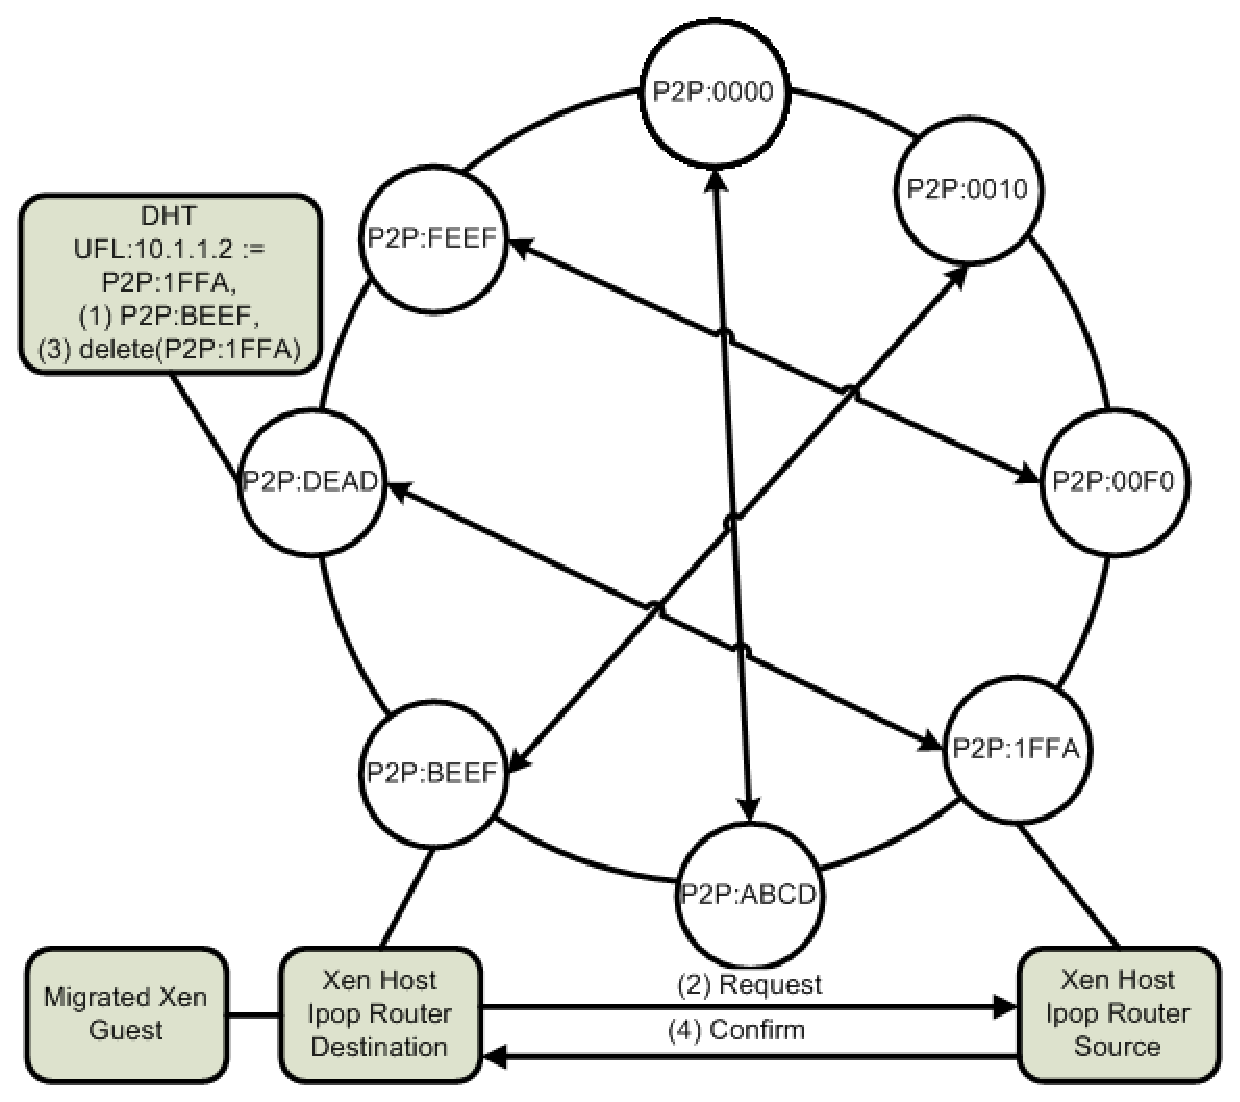
\epsfig{file=figs/Migration.png.eps, width=5in}
\caption[VN Router Migration]{The VN operations that occur after a guest (VM)
has been migrated.  (1) The destination retrieves the P2P information of the
source from the DHT and optimistically places its information into the Dht.
(2) The destination requests that the source delete its information from the
DHT.  (3)  The source confirms that the VM is no longer present and performs
the delete.  (4)  The source notifies the destination that its request has
finished successfully.}
\label{fig:migration_ring}
\end{figure}

\begin{figure}[ht]
\centering
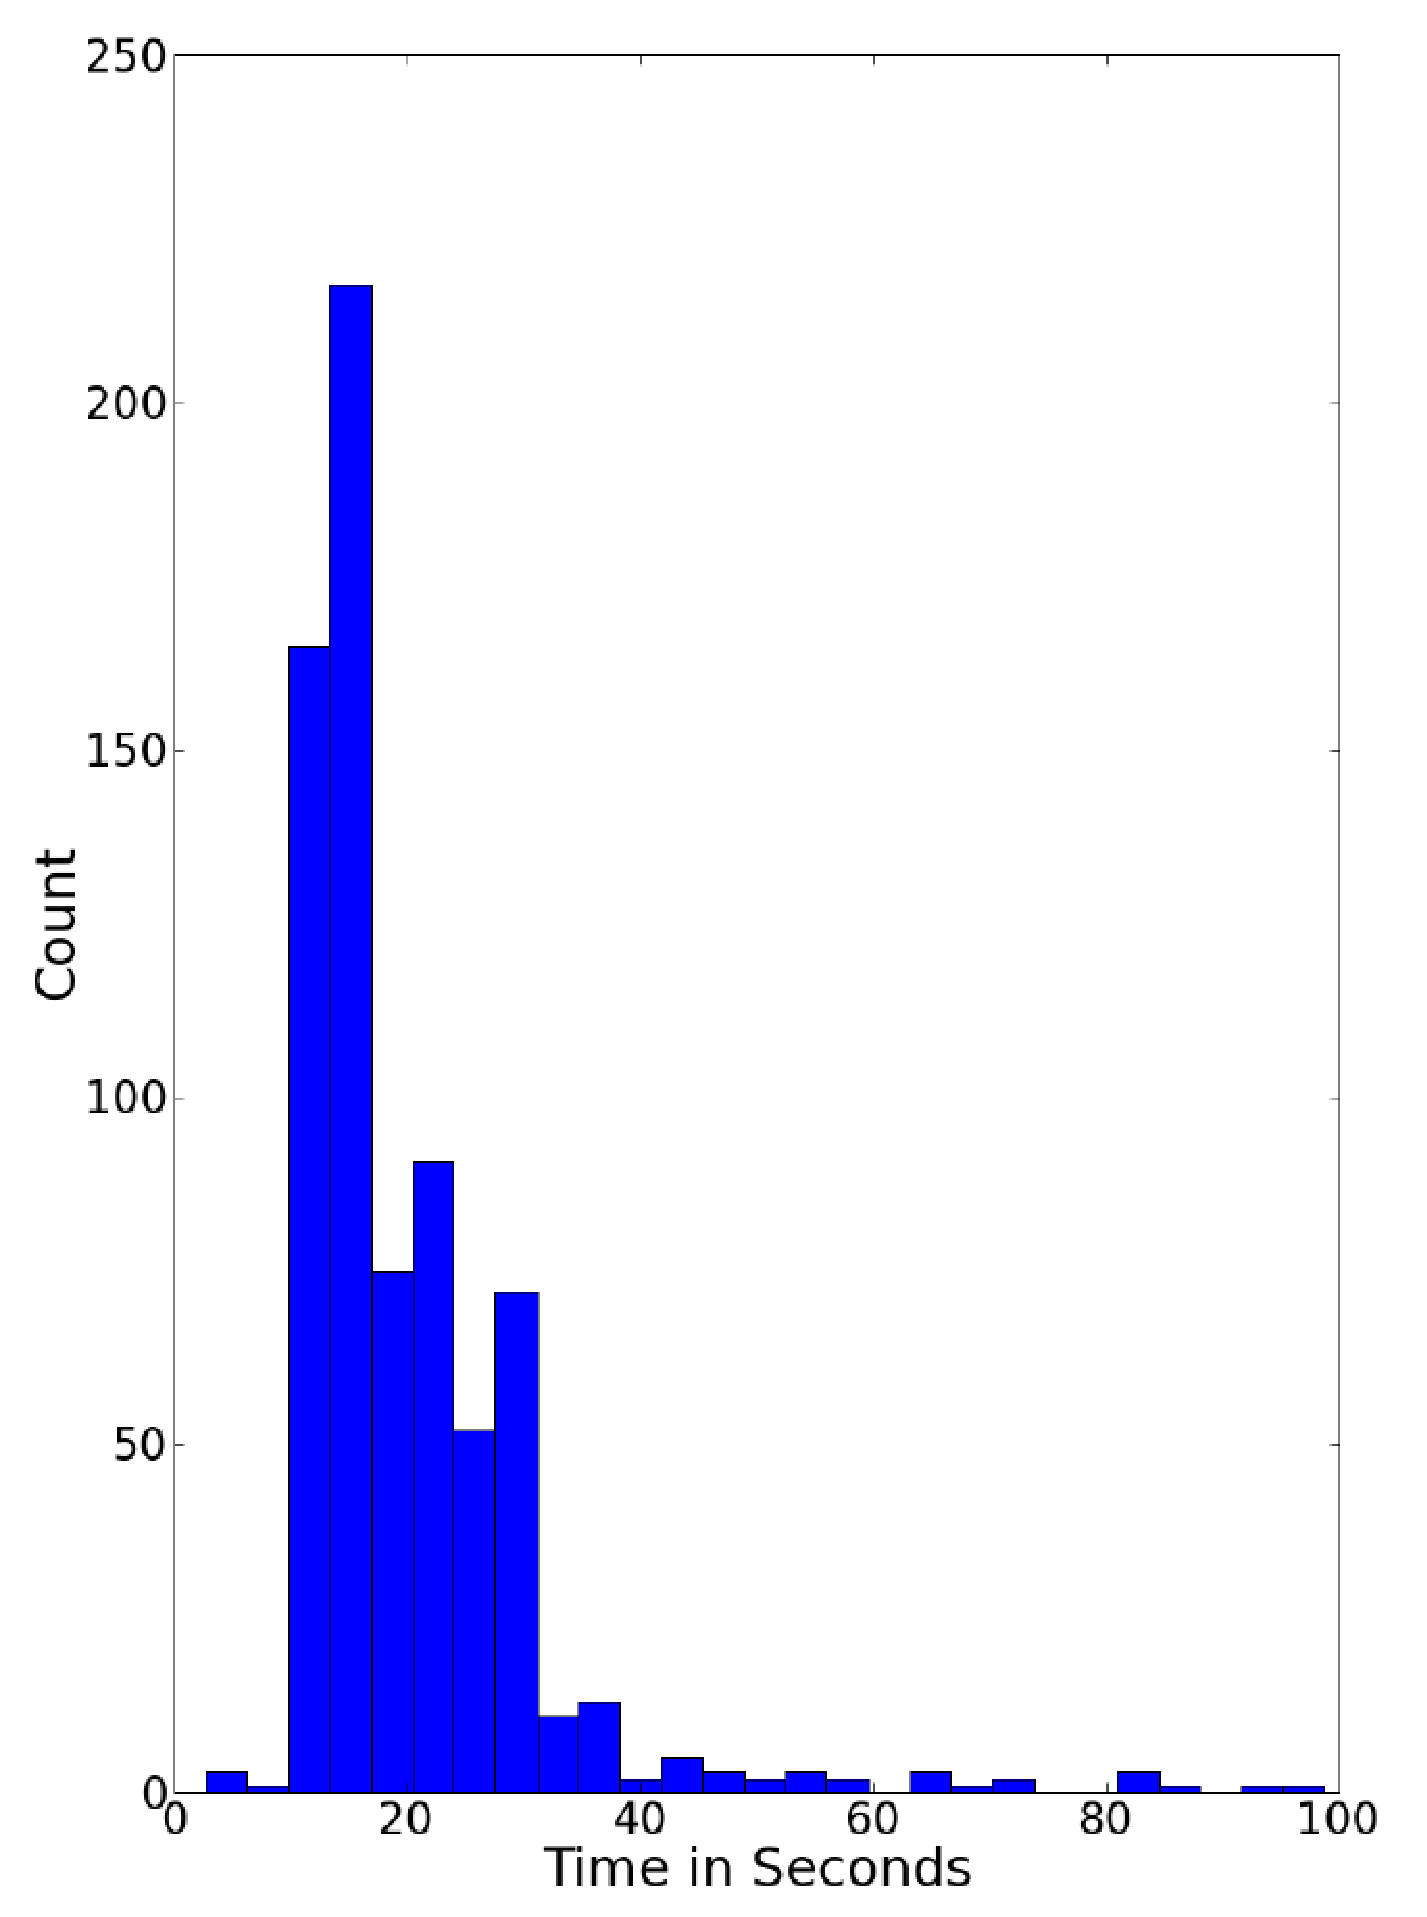
\epsfig{file=figs/migration_results.png.eps, width=2.5in}
\caption[VN Router migration evaluation]{VN Router migration evaluation.  Over
50 different IPs migrated about 10 times each.  The average was 20.11 seconds
with a standard deviation of 10.89.  In this experiment, the majority of this
time comes from VN migration, whereas VM migration requires less than a second.}
\label{fig:mig}
\end{figure}

\begin{figure}[ht]
\centering
\caption{Comparison of IP Broadcast and Multicast using overlay Broadcast and
Unicast.}
\label{fig:broadcast}
\end{figure}

\begin{figure}[ht]
\centering
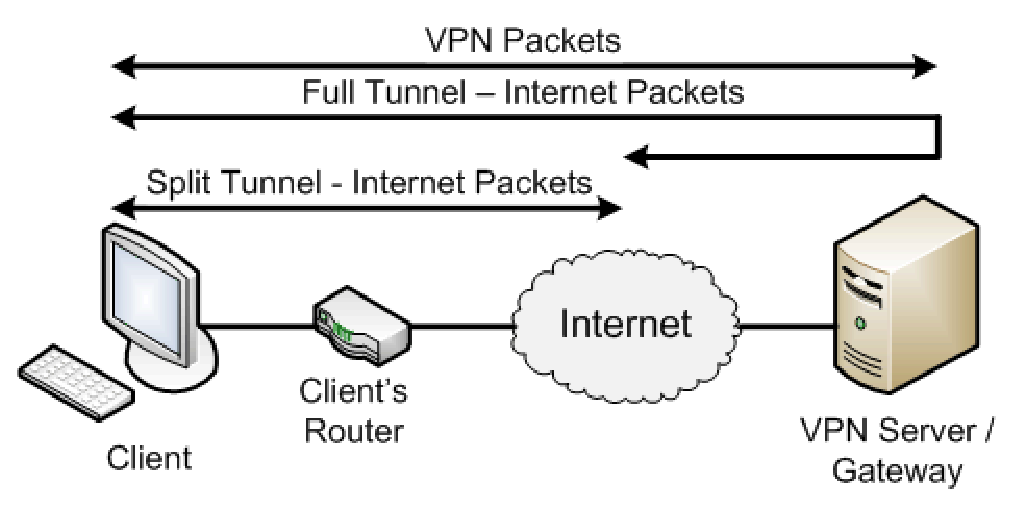
\epsfig{file=figs/tunnel.png.eps, width=4in}
\caption[An example of both full and split tunnel VPN modes]{An example of both
full and split tunnel VPN modes.  In both, packets for the server are sent
directly to the server.  In split tunnel mode, Internet packets bypass the VPN
and are routed directly to the Internet.  In full tunnel mode, Internet packets
are first routed to the VPN gateway, and then to their Internet destination.}
\label{fig:tunnel}
\end{figure}

\begin{figure}[ht]
\centering
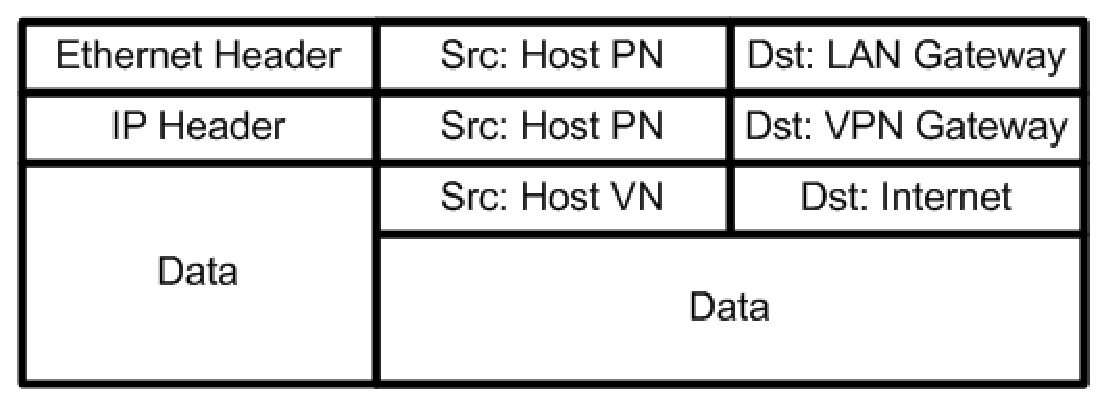
\epsfig{file=figs/tunnel_packet.png.eps, width=4in}
\caption[The contents of a full tunnel Ethernet packet]{The contents of a full
tunnel Ethernet packet.  PN and VN are defined as physical and virtual network,
respectively.}
\label{fig:tunnel_packet}
\end{figure}

\begin{table}[ht]
\centering
\begin{tabular}{|c||c|c|c|} \hline
& Google & GW Pri & GW Pub \\ \hline \hline
Ethernet & 70.6 & 12.9 & 13.9 \\ \hline
Routing & 71.4 & 13.2 & 11.0 \\ \hline
None & 66.1 & N/A & 10.9 \\ \hline
\end{tabular}
\caption[Full tunnel evaluation]{Latency results comparing full tunnel
approaches measured in ms.  Legend: GW Pri - gateway's VPN address, GW Pub -
gateway's VPN address, Ethernet - full tunnel Ethernet packet method, Routing -
full tunnel routing rule switch, None - split tunnel or no VPN.}
\label{tab:full_tunnel_eval}
\end{table}

\clearpage

\begin{figure}[ht]
\centering
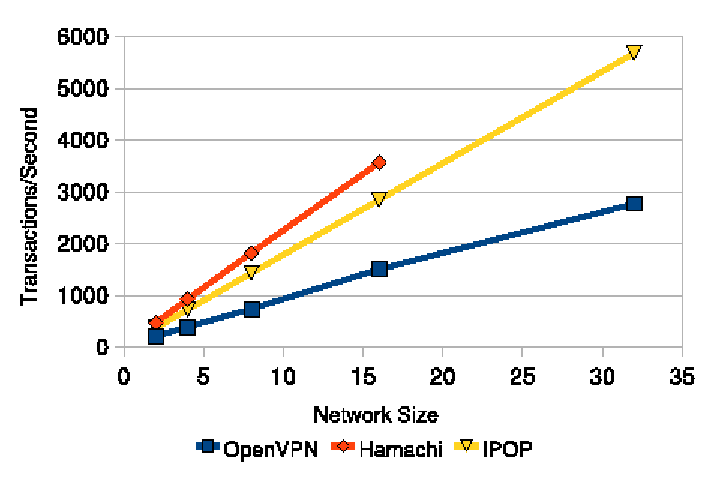
\epsfig{file=figs/latency.eps, width=4in}
\caption{System transaction rate for various VPN approaches.}
\label{fig:latency}
\end{figure}

\begin{figure}[ht]
\centering
\epsfig{file=figs/bandwidth.eps, width=4in}
\caption{System bandwidth for various VPN approaches.}
\label{fig:bandwidth}
\end{figure}

\begin{figure}[ht]
\centering
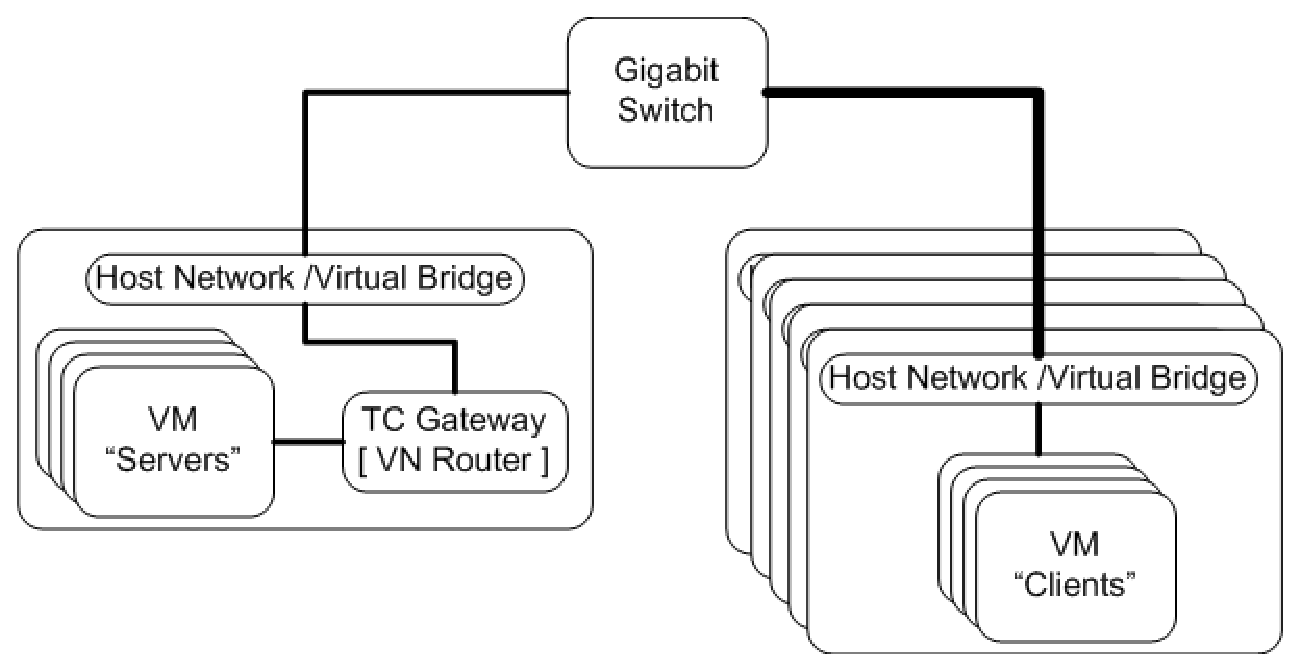
\epsfig{file=figs/grid_setup.png.eps, width=4in}
\caption[Grid evaluation setup]{The system setup for the grid experiments.  The
VM ``Servers'' ran SPECjbb and were also the site for the collection of the
netperf benchmarks.  All the VM ``Servers'' were connected through the TC
Gateway through host-only networking to the VM ``Clients''.  All traffic for
the VM ``Servers'' passes through the TC Gateway, which also doubled as the
Router in the Router experiments.}
\label{fig:gridsetup}
\end{figure}

\begin{figure}[ht]
\centering

\mbox{
\subfigure[TCP Stream bandwidth, SPECJbb load] {
  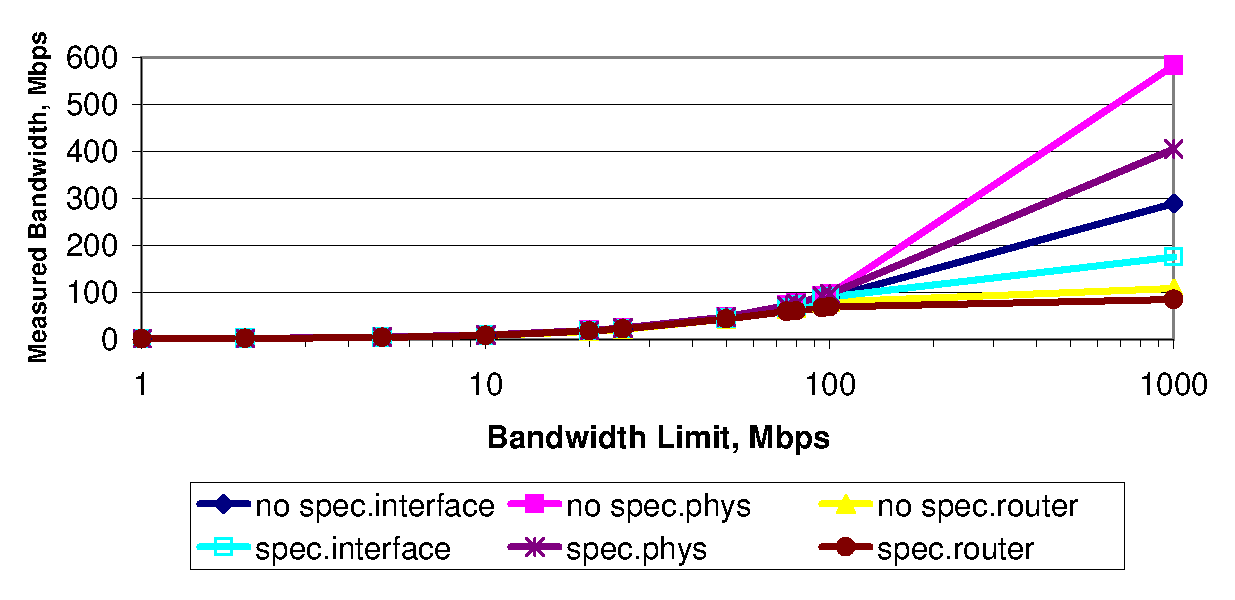
\includegraphics[width=.45\linewidth]{figs/stream.netperf.jpg.eps}
  \label{fig:stream.netperf}
}

\subfigure[TCP RR latency, SPECJbb load] {
  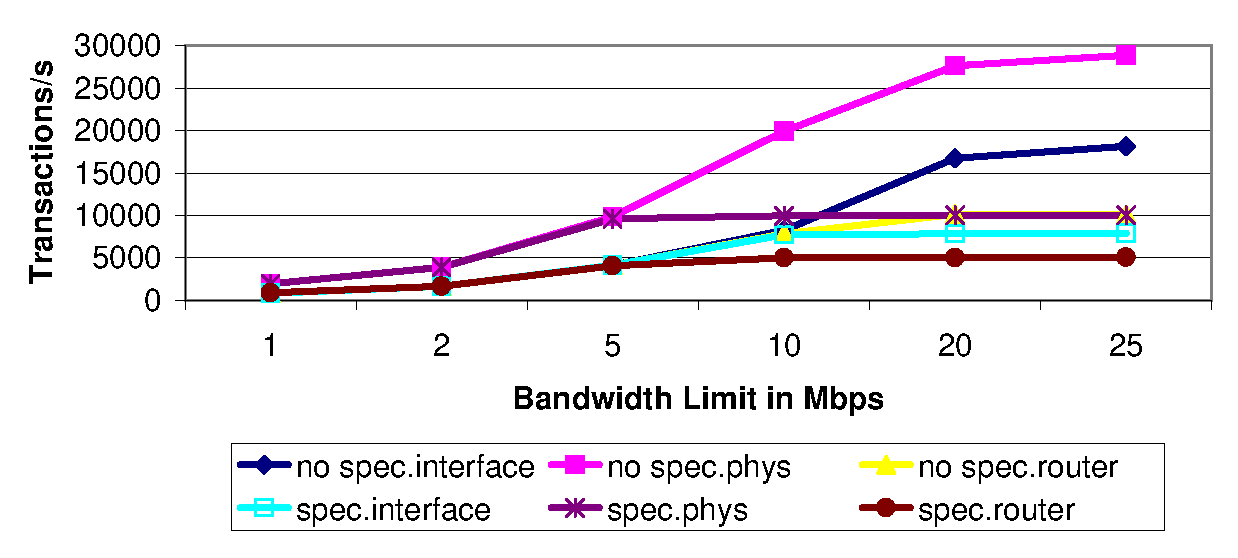
\includegraphics[width=.45\linewidth]{figs/rr.netperf.jpg.eps}
  \label{fig:rr.netperf}
}
}

\caption[Grid Netperf evaluation]{Netperf measurements with and without SPECjbb
load.  Lines are of the form (no spec, spec).(phys, interface, router).  Where
``spec'' indicates SPECjbb benchmark is active, while ``no spec'' indicates
that SPECJbb is inactive. ``phys'' implies the absence of IPOP with benchmarks
occurring directly over the ``physical'' network card.  ``interface'' and
``router'' present the results for VN interface and router models respectively.}
\label{fig:gridevalnet}
\end{figure}

\begin{figure}[ht]
\centering

\mbox{
\subfigure[SPECJbb score, TCP Stream load] {
  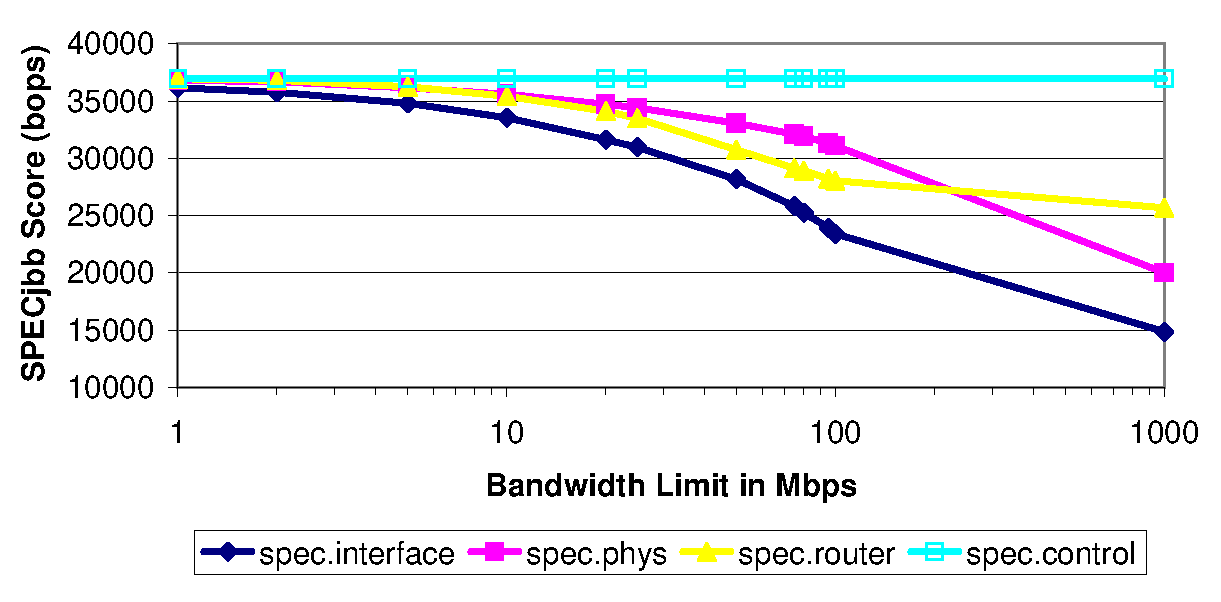
\includegraphics[width=.45\linewidth]{figs/stream.spec.jpg.eps}
  \label{fig:stream.spec}
}

\subfigure[SPECJbb score, TCP RR load] {
  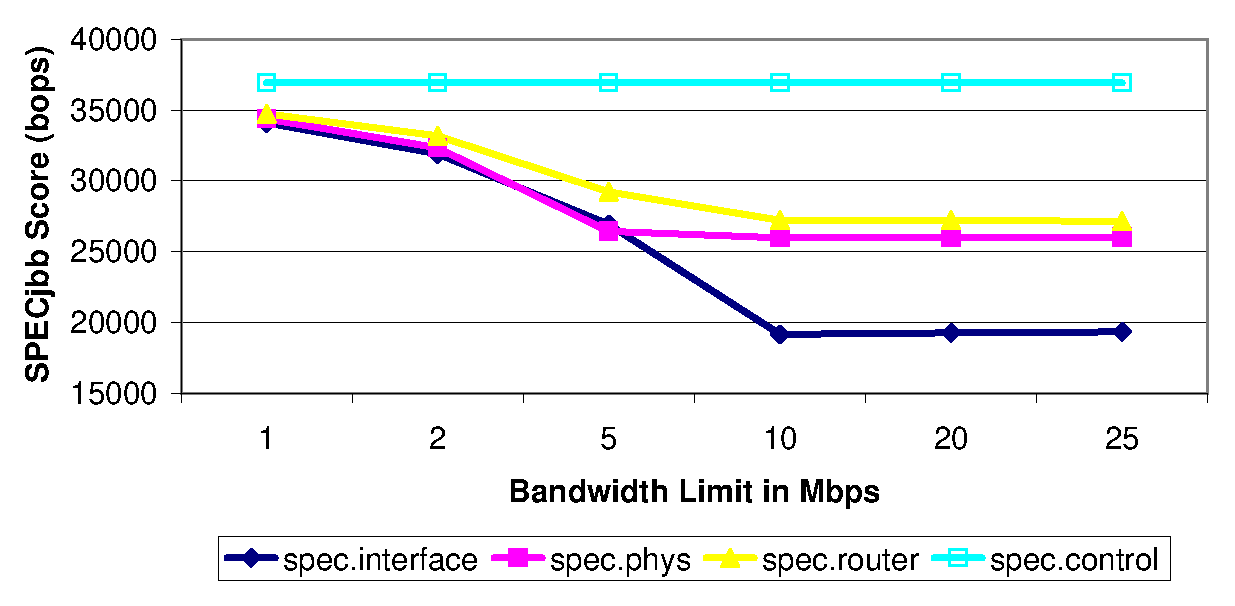
\includegraphics[width=.45\linewidth]{figs/rr.spec.jpg.eps}
  \label{fig:rr.spec}
}
}
\caption[Grid SPECjbb evaluation]{SPECjbb scores with and without Netperf load.
Lines are of the form spec.(control, phys, interface, router).  ``spec''
implies that SPECJbb executes in all tests.  In ``control'' Netperf is
inactive, that is, it is the maximum attainable value for SPECJbb. ``phys''
implies the absence of IPOP with benchmarks occurring directly over the
``physical'' network card.  ``interface'' and ``router'' present the results
for VN interface and router models respectively.}
\label{fig:gridevalcpu}
\end{figure}

\begin{table}
\centering
\begin{tabular}[c]{|l||c|c|c|} \hline
& EC2 / UF & EC2 / GoGrid & UF / GoGrid \\ \hline
Stream Phys & 89.21 & 35.93 & 30.17\\ \hline
Stream VN & 75.31 & 19.21 & 25.65\\ \hline
RR Phys & 13.35 & 11.09  & 9.97 \\ \hline
RR VN & 13.33 & 10.69 & 9.76 \\ \hline
\end{tabular}
\caption[WAN Results for inter-cloud networking]{WAN Results for inter-cloud
networking.  Stream is in Mbs and RR is in trans/s (The inverse of trans/s
would be equal to the average latency).}
\label{tab:cloud-wan}
\end{table}

\begin{table}
\centering
\begin{tabular}{|l||c|c|c|c|} \hline
 & VN Interface & VN Router & VN Hybrid & Physical \\ \hline
Stream & 109 & 325 & 324 & 327 \\ \hline
RR & 1863 & 2277 & 2253 & 3121 \\ \hline
\end{tabular}
\caption[LAN results performed at GoGrid]{LAN results performed at GoGrid.
Stream is in Mbs and RR is in trans/s.  Interface and Physical used the eth0
NIC, while Router and Hybrid used eth1.  Different VLANs may give different
results.}
\label{tab:cloud-lan}
\end{table}

\chapter{Grid Appliance}
High throughput computing (HTC) is a form of opportunistic computing that,
unlike high performance computing (HPC) seeking only powerful resources,
benefits from ad-hoc, arbitrary resources including computers found in computer
labs, homes, and offices as well as cloud resources and retired HPC clusters.
Creating and maintaining HTC systems that cross administrative domains (grids)
require expertise in networks, operating systems, and grid middleware to
configure the sites uniformly and guarantee connectivity amongst sites involved.

Administrators each have their own way of configuring resources and may be
hesitant or unwilling to configure resources in a way that conflicts with the
environmental norm.  This conflicts with the requirements of merging resources
across administrative domains as computing resources are typically configured
uniformly having a common environment and network rules.  Administrators would
prefer not having exceptional rules for a subset of resources under their
domain and do not want to grant access to lesser known, remote users.  Network
constraints such as firewalls and network address translation (NAT) can prevent
cross-domain communication.  With exceptions this may be ameliorated, but
additional rules may be required for each new cluster or resource added to the
cross-domain grid.

HTC clusters are not limited to large systems requiring dedicated
administrators: there are many systems that discuss the use of desktop or
opportunistic grids, such as Boinc~\cite{boinc} and PVC~\cite{pvc}.  While Boinc
solutions may be easily configured, the approach relies on a centralized
scheduler and that applications be compiled using Boinc API.  While PVC
enables parallel tasks and more decentralized system configuration, the
approach has scalability concerns and relies on a centralized node to assist in
node connectivity.  In general, there exists no solution that provides
scalable, self-configuring, decentralized grid systems for non-experts.

Connecting resources distributed across the Internet can be challenging due to
limit of IP (Internet Protocol) addresses available to an organization.  NAT
further complicates the issue by limiting the formation of direct links between
remote sites without external assistance.  When creating HTC systems across a
small set of institutions, approaches that use Internet Service Provider VPNs,
Layer 2 Tunneling Protocol (L2TP) VPNs, and other user-configured VPN
approaches can be used.  Most solutions require some form of centralization
and static links; as systems expand dynamically, the manual configuration of
the system grows significantly.  VPNs do, however, provide means of securing
the system and, through the use of proper middleware, can allow users to
interact with each others resources without additional configuration from the
local site administrator.

The Archer project~\cite{archer}, a collaborative academic environment
linking institutions and external users for the purpose of computer architecture
research, is an example of a real system having the described constraints.  Many
researchers have a need for resources occasionally and rather than investing
in a large pool of dedicated resources for a single institution they are able
to pool their resources together using HTC mechanisms.  The resulting system
allows individuals the opportunity to complete their jobs quickly and ensure
that their resource contribution is not idle when locally unused.  This use
case potentially introduces a new issue where the users may not be experts nor
have the ability to include an expert in the construction of the system.

Explicitly the requirements for a system in these environments are: 1) users
should be able to easily add and remove resources, 2) resources should not
require configuration to allow remote users access, 3) tasks that run inside
the grid should not have access to external resources, 4) external resources
should not be able to access the grid, 5) resource priority should be granted
to the resource's owner, and 6) malicious users should be able to be removed.
This chapter describes an approach to handling these requirements to
enable the creation of a dynamic, decentralized HTC grid through a novel
approach involving decentralized overlays enabling a self-configuring VPN
and HTC environment.  

In previous work, IPOP~\cite{ipop} was bundled with other grid middleware
into a virtual machine called the Grid Appliance~\cite{grid_appliance} for
easy to use decentralized virtual networking.  The approach was highly couple,
and while it made it easy to connect to existing grids to add or access
resources, it required expertise for users to create and manage their own
independent grids.  This paper extends that work to enable non-experts to
create and manage their own grids through a group-oriented model embodied in a
web 2.0 infrastructure providing a public key infrastructure along with VPN and
grid configuration.  The approach describes methods that can be used to easily
configure and combine resources from virtual, physical, and cloud
environments.

\section{Task Schedulers}
The most fundamental requirement of a cluster is the task scheduler.  Each
task scheduler has a general focus and selecting one that works well in a
specific environment can make the configuration of the system significantly
easier.  Generally, there are three approaches to configure HTC clusters: 1)
task workers pull from a centralized manager as employed by Boinc~\cite{boinc},
2) task workers receive jobs from a centralized submission site, and 3) task
workers receive jobs from any member of the HTC infrastructure.  Both 2 and 3
can be implemented using a myriad of different job schedulers with verifying
levels of difficulty.  Task schedulers supporting this behavior include
Condor~\cite{condor0}, Sun Grid Engine, and PBS and its relative Torque.

Unlike other task schedulers, Condor supports decentralized users supported
by having separate components that keep track of resources and negotiates
resource allocation from those that make the resource requests and submit
tasks.  This abstraction allows for a simple centralized system to maintain the
grid without requiring any run-time configuration.  In addition, Condor allows
open unauthenticated access to the grid as long as a peer is within a subnet.
Using a VPN ensures that that only members of the VPN have access to grid
resources.  To enable this behavior in other grid schedulers would require
modification or additional middleware, like Globus~\cite{globus_toolkit}.
Other reasons motivating the use of Condor include it being open source, having
an active community, and focus on opportunistic cycles.  In the list of
requirements, Condor also handles the ability to assign groups or institutions
privilege on their own resources when shared in a collaborative environment.
Condor supports multiple, decentralized negotiators through flocking.

Though settling on a task scheduler, it is important to present a comparison
of other features provided by task schedulers, as illustrated in
Table~\ref{tab:task_schedulers}.  Experience dictates that the approach
that requires the least amount of work to obtain the most amount of features is
ideal.  The important takeaway from manuals and experimental configuration of
various environments was that Condor can easily be configured to provide a
P2P-like scheduling environment, whereas other approaches were heavily
centralized.  While they could be decentralized and each had their own benefits
that it did not outweigh the ease of use provided by Condor.

\section{P2P VPNs}
Many of the requirements described can be addressed through the use of a
VPN.  A VPN can assist in dealing with connecting network constrained resources,
securing the grid from the outside world, and removing malicious forces inside.
Grid computing has seen its fair share of VPNs such as ViNe~\cite{vine},
Violin~\cite{violin}, and VNET~\cite{vnet}.  These approaches are limited by
their lack of self-configuration, namely that static links between peers must
be created, security credentials must be manually distributed, and lack of
support for direct connectivity between NAT and firewalled peers without
additional configuration from the user limiting their applicability for such
resources to communicate with each other through proxy servers.  In
PVC~\cite{pvc}, the authors describe an approach that self-configures through
a centralized server with NAT traversal support, which works on many
NAT devices but only when used without a stateful firewall.  The drawbacks with
this approach are the centralized key distribution center (KDC) and lack of
encrypted links.

IPOP~\cite{ipop} provides a P2P virtual network with decentralized and
self-configuring link creation with NAT traversal support that works with
most NATs using a distributed hash table (DHT) for address
allocation and resolution.  Previous approaches~\cite{grid_appliance} used
IPsec for security or went without it entirely as IPOP lacked the ability to
secure links.  Chapter~\cite{vpns} presents GroupVPN, which transforms IPOP
into an automated VPN with enhanced NAT handling through the use of
decentralized relays (proxies), enabling two-hop, low latency connections when
NAT and firewall traversal fails.

The authentication system employs a public key infrastructure (PKI), made
accessible through a group-based Web 2.0 environment.  Users can create and
join groups, and group owners can grant user access, promote users to
administrative capabilities, or remove users who have overstayed their
welcome.  A PKI has a very natural P2P aspect, in that, peers can mutually
authenticate each other by verifying signatures on the exchanged certificates
unlike the centralized authentication such as a KDC.  To automatically configure
the system, users download a GroupVPN configuration file through the group
website, which can be provided to the GroupVPN by command-line or GUI.  The
next time GroupVPN is started, it will use this configuration to automatically
obtain a signed certificate by sending a certificate request along with a
shared secret contained in the configuration to the group server through HTTPS,
uniquely authenticates the user.  If the user has appropriate permissions, the
server will sign the certificate request.  To remove peers, the system supports
a reliable, centralized user revocation list located at the group website and
decentralized revocation by broadcast and distributed data stores.

\section{GroupAppliances}
An appliance is defined as a dedicated, blackbox device requiring little if any
configuration from the user.  While traditional computing appliances like a
router, network storage, or even cluster resources have been available as
hardware appliances, the recent resurgence of virtualization initiated by
VMware and Xen has made software appliances by means of virtual appliances
popular.  Recently, cloud computing has become popular in large part thanks to
Amazon's EC2.  Both virtual and cloud resources present themselves as cheap
computing for HTC and opportunistic computing purposes, because they can be
setup in such a way as to have no or limited effect on users' computers and can
be shutdown when no longer in use.  Even with virtual and cloud appliances 
available to tap into these resources, they still require some manual
manual configuration to form a grid, and these packaged solutions cannot easily
be applied to hardware resources.

Our solution is the creation of a generic software stack that self-configures
based upon a user input configuration file.  The contents of a configuration
file are the type of resource (dedicated compute node, job scheduling node, a
mixture of the two, or the job negotiating central server); the user's group and
username on the site; and the grid's GroupVPN configuration data.  The
configuration file is generated from a Web 2.0 group-based infrastructure
called GroupAppliance, using a single GroupVPN group to connect all members of
the grid together in a VPN but using the GroupAppliance group to distinguish
their resource contributions.  Thus many GroupAppliances groups can be linked
together through a GroupVPN group.  By distinguishing resource contributions,
users are able to get credit and gain priority to their resources when
submitting tasks to run.

When a user downloads the configuration file from the GroupAppliance
infrastructure, the data is stored in a floppy disk image that can be used on
physical resources by writing the image to a real floppy disk or to a USB drive,
a VM by adding a virtual disk image to the VM, and clouds through instance
specific configuration data.  EC2 provides per-cloud instance configuration in a
parameter called ``user data'' providing up to 16 KB of data available only to
that cloud instance.  At the time of this writing, it appears that EC2 is the
only cloud provider to offer this option.  Alternatively, users could configure
an image specifically to run for this cloud by inserting the floppy image into
the cloud image and then generating cloud instances from this new image, or the
user could setup a storage cloud where the cloud instances could retrieve the
floppy.  Because the floppy contains private GroupVPN configuration data it
should not stored on public resources.

Upon booting, the grid configuration scripts parse the floppy to determine how
to configure the machine.  Negotiators insert an ad into the DHT, whereas
resources and task submitters query the DHT for the list of negotiators,
selecting one and relegating the rest for flocking.  At which point, tasks
can be submitted and run.

\section{Constructing Environments}
Often VMs are favored for the distribution of complicated applications as
experts can configure them and release the results as a complete working system.
This approach may limit non-expert use to the VM appliance, which may be
undesirable for users that want to configure their own systems without reuse
of the existing VM.  Guides may exist for the creation of systems, most
systems are too complex for non-experts to produce similar results found in the
VM.  In addition to supplying VMs, providing packages (DEB and RPM) enable easy
installation in arbitrary environments and through the use of package
managers (APT and YUM) handle configuration such that the requirements listed
in the introduction are handled.  Packages can be provided that automatically
install and configure the task scheduling middleware and a VPN as well as
sandbox the environment, limiting users network access to the virtual network
and not external networks such as other local resources and the Internet.  The
remaining components are configurable through the GroupAppliances interface and
decentralized through the DHT.

The most important components in securing an environment are limiting internal
and external access from inside the system.  Specifically, internal resources
have no password enabled accounts to avoid cases where users submit tasks that
attempt to provide more privileged access to the user.  In the event that a
passworded account is necessary, such as on a client machine, the system is
configured to prevent permission switching by the task scheduler user, in
Linux, for example, this is done by limiting \textit{su} access.  By default,
Condor runs jobs as either nobody or the user named ``Condor''.  This limits
access to many of the core components of the system already, but it does not
limit the users ability to read files that allow reading from anyone on the
system and the ability to communicate to external resources from inside the
machine.  The user data directory is made readable by only the user and group
who own the files and directories preventing remote users from reading local
user personal data.  Limiting access to external resources has been implemented
by a firewalling, allowing the Condor user to only have the ability to send
packets over the virtual network.

Job submission nodes have an additional consideration emphasizing
user-friendliness.  To do this, file system access through NFS and Samba
as well as remote access through SSH are enabled to allow users on the same
host can access the resources without having to configure additional utilities
or using the VMs interface.  To prevent access through the virtual network or
Internet for security purposes, a second network card connects the system to
a host-only interface.  By binding all user applications to use the network
interface, they do not require extra security enhancements.  Alternatively,
applications like SSH could be enabled to only allow private key based login.
In general, only dedicated compute nodes and possibly the job negotiator will
run on physical or cloud resources, whereas clients will most likely
exclusively use VMs.

preparing the system is straight-forward: users configure the package manager to
link to a package distribution site and then install the desired packages for
the grid resource.  When finished, the user can restart the device or restart
the grid service with the floppy image adding a new resource to the grid.  The
VPN will acquire a signed certificate and grid configuration scripts will
configure Condor and other services through interaction with the DHT.

\section{Related Work}
\label{related_work}
There are many projects that seek to provide easy to use resources for HTC
and opportunistic computing.  We focus on two approaches whose focus is
user-friendly dynamic grids: PVC~\cite{pvc} and GPU~\cite{gpu}.

PVC or Private Virtual Clusters creates instant grids using a PVC specific
virtual network and task scheduler as well as VMs to isolate remote jobs from
users' resources.  Resources discover and TCP NAT traversal are performed
through a centralized system broker, though it is unclear how the resources are
configured with the knowledge of the broker, nor how a broker is configured.
Loss of the broker can prevent usability of the system.  PVC virtual network
lacks privacy, links are authenticated through a KDC but messages are not
encrypted or authenticated.  PVC scalability constraints are unclear, as
experiments were limited to 8 nodes.  In contrast, our approach focuses on
privacy, scalability, and self-configuration through a decentralized system.

GPU or Global Processing Unit uses the Gnutella P2P system to create a
completely decentralized computing grid.  The authors state that the expected
size for grids range from 5 to 15 nodes.  While the authors do not mention NAT
traversal, there are many Gnutella systems that do support various forms of it.
There is no mention of providing safety to the users' resources from malicious
tasks.  While GPU provides easy configuration, it lacks the ability to run
jobs in a sandbox and support large pools of resources.

There are many other desktop grid environments that use Boinc as the underlying
method to push jobs.  As explained earlier, Boinc uses a few approaches that
are undesirable for our requirements with the primary issue that Boinc job
scheduling is heavily centralized.  In addition, for Boinc systems that allow
running arbitrary applications, it is unclear how secure they are.

\section{Evaluation}
\label{evaluation}
This evaluation evaluates the validity of this approach by evaluating the time
time required to create and utilize a grid consisting of various distributed
resources using a reference implementation of the system described in this
paper.  Using VMware resources behind a Cisco and ``iptables'' NAT at the
University of Florida (UF), KVM resources behind an ``iptables'' and KVM NAT at
Northeastern University (NEU), and cloud resources provided by EC2, pools of 50
resources from each site were booted independently and then together, resulting
in 4 different test runs.  The resources connect to an existing pool consisting
of a negotiator and client node.  Once all the resources have connected, the
client submits a job to each resource.  Three timespans are measured: ``start''
- begins with starting the experiment including the copying of files and
creation of instances until all resources have been powered on, ``connect'' -
begins with ``start'' though ends when all resources appear in
``condor\_status'' and includes start time, and run - time from the submission
to the conclusion of a 5 minute job to all resources Like connect, run measures
the time for VPN connections, only from the client to the resources instead of
from the negotiator.  All tasks are automated through scripts with human
interaction required only to start the events of grid boot and job submission.
Results are presented in Figure~\ref{fig:results}.

As the systems consist of various hardware and software configurations, the
time to start is provided as a basis for the remaining numbers.  Some of the
interesting experiences of the experiment were:  1) the combination of the
``iptables'' and VMware NAT was more easily traversable than the combination
of ``iptables'' and KVM NAT and 2) in the experiment consisting of 150 peers,
nodes were actually well connected much earlier, but due to missed packets and
Condor timeouts, not all resources were accounted for in Condor as early as in
the other tests.

\section{Real Use Cases}
There are several deployments using the system described.  Over the past 2
years, I have been student lead in an active grid deployed for computer
architecture research, Archer~\cite{archer}.  Archer currently spans four
universities with 500 resources, we have had hundreds of students and
researchers submitting jobs with over 150,000 hours of total job execution in
the past year alone.  Groups at the Universities of Florida, Clemson, Arkansas,
and Northwestern Switzerland have used it as a tool to teach grid computing.
Purdue is constructing a large campus grid using GroupVPN to connect resources
together.  Recently, a grid at La Jolla Institute for Allergy and Immunology
went live with minimal communication with us.

\begin{table}[ht]
\centering
\caption{Task scheduler comparison}
\label{tab:task_schedulers}
\end{table}

\begin{table}[ht]
\centering
\begin{tabular}{|c||c|c|c|c|} \hline
& 50 - EC2 & 50 - NEU & 50 - UF & 150 - All \\ \hline\hline
Start & 2:44 & 10:21 & 20:23 & 21:14 \\ \hline
Connect & 5:10 & 21:47 & 24:16 & 38:27\\ \hline
Run & 7:15 & 6:35 & 5:53 & 21.19 \\ \hline
\end{tabular}
\caption[Grid creation times]{Time in minutes:seconds to start and connect
resources to an existing grid and run jobs from.}
\label{fig:results}
\end{table}


\chapter{Social Profile Overlays}
\label{spo}
Online social networking has become pervasive in daily life, though as social
networks grow so does the wealth of personal information that they store.  Once
information has been released on a social network, known as a user's profile,
the data and the user are at the mercy of the terms dictated by the social
network infrastructure, which today is typically third-party, centrally owned.
If the social network engages in activities disagreeable to the user, due to
change of terms or opt-out programs not well understood by users such as recent
issues with Facebook's Beacon program~\cite{facebook_beacon}, the options
presented to the user are limited: to leave the social network (surrendering
their identity and features provided by the social network), to accept the
disagreeable activities, or to petition and hope that the social network
changes its behavior. 

As the use of social networking expands to become the primary way in which users
communicate and express their identity amongst their peers, the users become
more dependent on the policies of social network infrastructure owners.  Recent
work~\cite{p2p_socialnetwork} explores the coupling between social networks and
P2P systems as a means to return ownership to the users, noting that a social
network made up of social links is inherently a P2P system with the aside that
they are currently developed on top of centralized systems.  In this paper, we
extend this idea with focus on the topic of topology; that is, how to
self-organize social profiles that leverage the benefits offered by a
structured P2P overlay abstraction.

Structured P2P overlays provide a scalable, resilient, and self-managing
platform for distributed applications.  Structured overlays enable users to
easily create their own decentralized systems for the purpose of data sharing,
interactive activities, and other networking-enabled activities.  This work
extends Private Virtual Overlays described in Chapter~\ref{vpo}.  This chapter
expands upon this approach with in-depth discussion on how to apply this
technique to enable social network overlay profiles.

Social networks consist of users, each has a profile, a set of friends, and
private messaging.  The profile contains user's personal information, status
updates, and public conversations, similar to a message board.  Friends are
individuals trusted sufficiently by a user to view the user's profile.  Private
messaging enables sending messages discretely between users without leaking the
message to other members.  Using this model, we describe how a public overlay
can be used as a directory for finding friends and joining existing profile
overlays.  Each user has their own profile overlay, secured via a public key
infrastructure (PKI) to which they are the certificate authority (CA).  The
profile overlay stores profile data in its distributed data store, supporting
profile access in scalable mechanisms regardless of the profile owner's online
status.  This chapter explains architecture of these overlays, presented in
Figure~\ref{fig:system}, how they are used to find and befriend peers, and
describes approaches to handling profile data and establishing initial
connections to profile overlays.

\section{Peer-to-Peer Social Networks}
In~\cite{peerson}, a DHT provides the look-up service for storing meta data
pertaining to a peer's profile. Peers query the DHT for updated content from 
their friends by hashing their unique identifiers (e.g. friends' email
addresses).  The retrieved meta data contains information for obtaining the
profile data such as IP address and file version. Their work relies
on a PKI system that provides identification, encryption, and access control.
In contrast, our approach provides each user their own private overlay secured
by point-to-point encryption and authentication amongst all peers in the profile
overlay.  The profile overlay provides a clean abstraction of access control,
whereby once admitted to a private overlay, users can access a distributed data
store which holds the contents of the owners profile.

\cite{vis-a-vis} takes a different approach by depending on virtual individual
servers (VIS) hosted on a cloud infrastructure such as Amazon EC2. Friends
contact each other's VIS directly for updates.  A DHT is used as a directory for
groups and interest-based searches. Their approach assumes bidirectional
end-to-end connectivity between each VIS, where a profile is only available
during the up time of the VIS.  Because of the demands on network connectivity
and up time, the approach assumes a cloud-hosted VIS and has difficulty being used on user-owned resources.
Our approach enables users to avoid the need for all-to-all connectivity and
constant up time through the use of NAT traversal support and the
ability to store the profile in the overlay's distributed data store.

The approach presented in~\cite{matryoshka} also uses a DHT for looking up a peer's
 circle of friends.  Once a node in the peer's
outermost circle is found, that node is used to route profile requests to the
innermost circle which contains replicas of a peer's profile. Trust is enabled
through the use of an identification service contacted through the DHT.  The
circle of friends concept lacks the simplicity of the abstraction made in our
approach, which can easily be applied to existing structured overlays
unlike the concept of innermost and outermost circles.  Our approach
also enables the profile owner to serve as a CA, ensuring that nodes can only
access a profile overlay after having obtained a signed certificate.  

Unlike the above approaches, the P2P social network presented in~\cite{tribler-osn}
uses an unstructured overlay without a DHT where peers connect directly to
each other rather than through the overlay establishing unique identifiers to
deal with dynamic IPs.  Peers cache each other's data to improve availability.
While helper nodes are used to assist with communication between peers behind
NATs.  The approach lacks security and access control considerations and lacks the
guarantees and the simplicity of the abstraction offered by a structured overlay.

\section{Social Overlays}
\label{social_overlays}
In this section, we explain how to map online social networking to our
multi-overlay social network consisting of a public directory overlay with many
private profile overlays.  The directory overlay supports friend discovery and
verification and stores a lists of peers currently active in each profile
overlay.  Profile overlays support message boards, private messages, and media
sharing.

\subsection{Finding and Verifying Friends}
In a traditional social network, a directory provides the ability to search
for users using public information, such as the user's full name, user ID,
e-mail address, group affiliations, and friends.  The search results return zero
or more matching directory entries.  Based upon the results, the user,
\textit{A}, can potentially make a friendship request.  The request receiver,
\textit{B}, can review the public information of A to making a decision.  If
\textit{B} accepts the request, \textit{A} and \textit{B} are given access to
each other's profiles.  Once profile access has been enabled, the users can
learn more information, and if it turns out to be a mistake, the peers can
unilaterally end the relationship.

To map this to our proposed social overlay, the directory entries would be
inserted into the DHT of a public overlay.  As discussed in previous work, the
DHT keys for these entries should consist of a subset of the user's
public information in lower-case format and hashed to an overlay  address.  The
value stored at these keys is the user's certificate, which consists of its public
information and an overlay address where the user expects to receive
notifications.  This overlay address can be used for asynchronous offline
messaging, whose function we will explain shortly.

Because the users need a way to verify each other that involves social credentials,
we propose the use of a new form of certificate.
The main portion of the certificate is similar to a self-signed
x509 certificate with public information such as user's name, e-mail
address, and group affiliations embedded into the certificate.  At the tail of
the certificate is a friend list represented by many friend entries.  To do this
we propose employing a technique similar to PGP: users can acquire from their
friends a signed message consisting of a hash of the peer's certificate, the
time stamp, and the friend's certificate hash signed by the friend.  Since PGP
does not provide a strong method for revocation, the time stamp provides
additional information to help decide whether or not a friendship link is still
active without accessing the profile overlay of either peers.  Peers should
request a new friend list entry within a certain period of time or it will
appear that the friendship is no longer valid.

While looking for an individual, a peer may discover that many individuals have
overlapping public information components, such as the user's name.  Assuming
all entries are legitimate, the overlay must have some method of supporting
multiple, distinct values at the same key, leaving the peer or the peer's DHT
client to parse the responses and determining the best match by reviewing the
contents of each certificate.  Alternatively, a technique like
Sword~\cite{sword}, which supports distributing the data across a set of nodes
and using a bounded broadcast to discover peers that match all information,
could be used for searching.

If a peer, \textit{A}, desires a friendship with another peer, \textit{B},
\textit{A} issues a friendship request, which will be stored in the DHT
at the overlay address listed in \textit{B}'s certificate, as described earlier.
The friendship request consists of the self-signed certificate of
\textit{A}, the requesting peer; the public information of the request receiver,
\textit{B}; and a time stamp; all signed with the private key associated with 
\textit{A}'s private key matched to their self-signed certificate.
% Though because DHTs are soft state systems having
% leases, the requester must reinsert the request upon timeout and no response for
% the receiver.

Within a reasonable amount of time after a request has been inserted into the
DHT, \textit{B} can come online and check for outstanding requests.  Upon
receiving a request, \textit{B} has three choices: a conditional accept, an
unconditional accept, or a reject.  During an unconditional accept, \textit{B}
signs \textit{A}'s request and issues a request to befriend \textit{A}.
Alternatively in the case of a conditional accept, \textit{B} issues a friendship
request, waits for a reply, and investigates the profile prior to signing the
\textit{A}'s request.  Once a user has received a signed certificate,
they may access the remote peer's profile overlay as discussed
in~\ref{profile_overlay}, which is also responsible for activities such as
revocation.

%Since a DHT is a soft-state system that uses leases to remove expired data, requests
%and responses must be occassionally reinserted into the DHT.  Alternatively, the
%approaches mentioned in~\cite{} that suggest methods of storing data in overlays
%using quotas could be used to ensure fair usage of the overlay.

\subsection{The Profile Overlay}
\label{profile_overlay}
In a traditional social network, the profile or user-centric portion consists
of private messaging, data sharing, friendship maintenance, and a
public message board for status updates or public messages.  In this
section, we explain how these components can be applied to a structured overlay
dedicated to an individual profile.

Using the techniques such as those described in~\cite{icdcs10}, it is feasible
to efficiently multiplex a P2P system across multiple, virtual private overlays enabling
each profile owner to have a profile overlay consisting of their online friends.
For access control, we employ a PKI, where each member uses the signed certificate
generated during the ``finding and verifying friends'' stage.  All links are
encrypted using symmetric security algorithms established through the PKI,
thus preventing uninvited guests from gaining direct access to the overlay and
hence the profile.  Because the profile owner also is the CA for all members of
the overlay, they can easily revoke users from access to the profile overlay.
In ~\cite{icdcs10}, we described mechanisms for overlay revocation through the
use of broadcasting for immediate revocation and the use of DHT for indirect
and permanent revocation.

The message board of a profile can be stored in two ways: distributed within the
profile overlay via a data store or stored on the profile owner's personal
computing devices.  The distributed data store provide the profile when the
owner is offline and also distributes the load for popular profiles.  For
higher availability, each peer should always be a provider for all data in their
profile when they are online.  To ensure authenticity and integrity, all peers
should sign their messages and each peer's certificate should be available in
the overlay for verification.  Messages that are unsigned should be ignored
by all members of the overlay.  An ideal overlay for this purpose should
support complex queries~\cite{complex_queries} allowing easy access to data
stored chronologically, by content, by type, i.e., media, status updates,
or message board discussions.

Private messaging in the profile overlay is unidirectional meaning that only
the profile owner can receive private messages using their overlay.  To
enforce this, a private message should be prepended with a symmetric key
encrypted by the profile owners public key, the message should be appended
by a hash of the message to ensure integrity and the entire message encrypted
by the symmetric key.  This approach ensures that only the sender and the
profile owner can decrypt the private message.  The contents of the private
message should include the sender, time sent, and the subject.  Messages can
be stored in well known locations, so that the profile owner can either poll
the location or, alternatively, use an event based system to notify them of
the new message.

\subsection{Active Peers}
The directory overlay should be used to assist in finding currently active peers
in the profile overlays.  By placing their node IDs at a well-known, unique
per-profile overlay keys in the DHT, active peers can bootstrap incoming peers
into the profile overlay.  We implemented and evaluated this concept
in~\cite{icdcs10}.  Because the profile overlay members all use PKI to ensure
membership, even if malicious peers insert their ID into the active list, it
would be useless as the peer would only form connections with peers who also
have a signed certificate.

\section{Challenges}
\label{outstanding}
While structured P2P overlays have been well-studied in a variety of applications,
their use in social profile overlays raises new interesting questions, including:

{\bf 1) Handling small overlay networks} - P2P overlay research typically focuses on
networks larger than the typical user's friend count (Facebook's average is
130\footnote{http://www.facebook.com/press/info.php?statistics}).  Because social profile overlays are comparatively smaller, this can
impact the reliability of the overlay and availability of profile data.  A user
can host their own profile; however when the user is disconnected it is important
that their profile remains available even under churn. It is thus important to
characterize churn in this application to understand how to best approach this
problem. An optional of per-user deployment of a virtual individual server (VIS)
and the use of replication schemes aware of a user's resources provide possible
directions to address this issue.

{\bf 2) Overlay support for low bandwidth, unconnected devices} - devices such as
smart phones cannot constantly be actively connected to the overlay and the
connection time necessary to retrieve something like a phone number may be
too much to make this approach useful.  Similar to the previous challenge,
this approach could benefit from using a VIS enabling users access to their
social overlays by proxy without establishing a direct connection to the overlay
network.

{\bf 3) Reliability of the directory and profile overlay} - Overlays are
susceptible to attacks that can nullify their usefulness.  While
the profile overlay does have point-to-point security, in the public,
directory overlay, the lack of any form centralization makes policing the system
a complicated procedure.  While our approach of appending friends list can assist
users in making decisions on identity, it does not protect against denial of
service attacks.  For example, users could attempt create many similar identities
in an attempt to overwhelm a user in their attempt to find a specific peer.
Previous work has proposed methods to ensure the usability of overlays even
while under attack.  For the social overlay to be successful, we must identify
which methods should be used. A possible approach is to replicate public
information within a user's profile overlay thus providing an alternative
directory overlay for querying prior to using the public directory overlay.

\section{Figures and Tables}

\begin{figure}[ht]
\centering
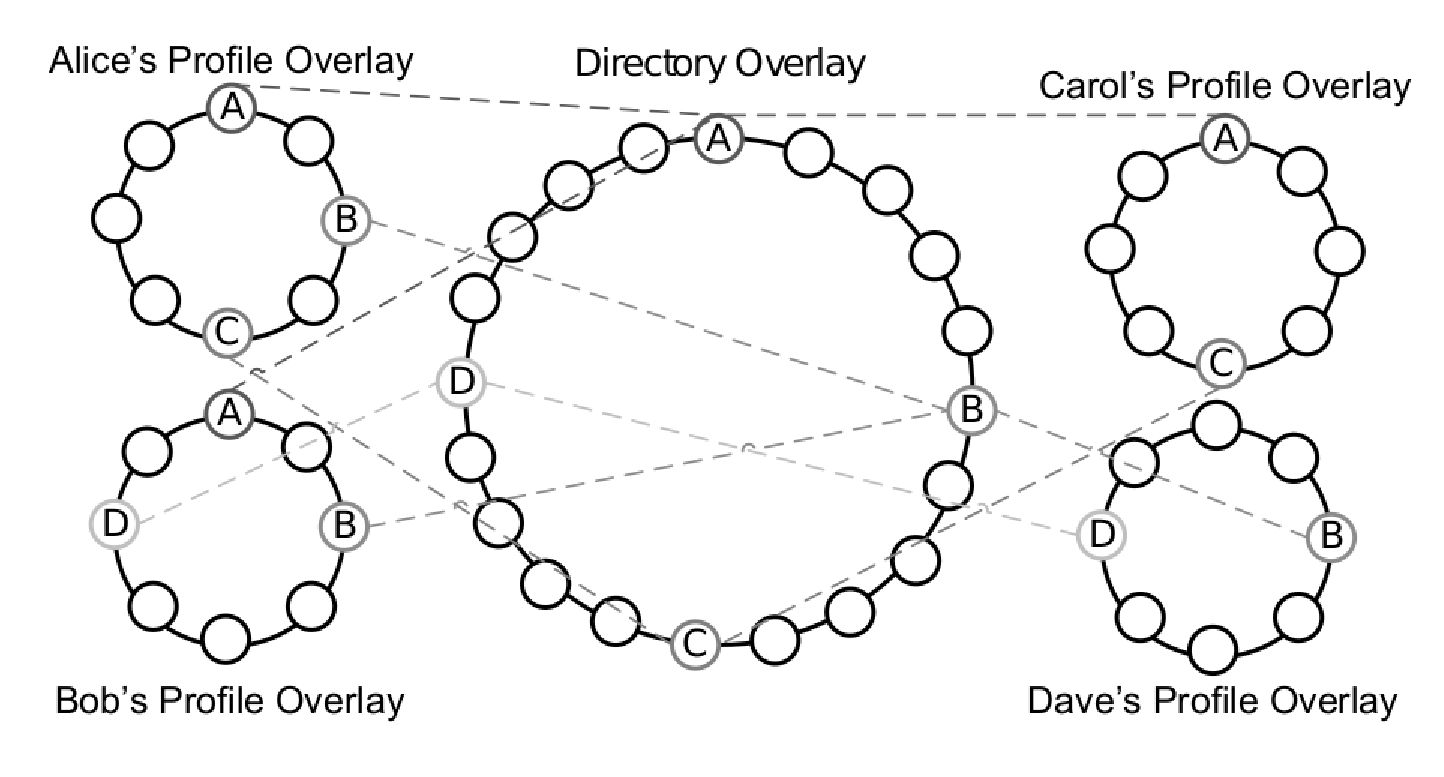
\epsfig{file=figs/subrings.eps, width=3.12in}
\caption{An example social overlay network.  Alice has a friendship with Bob and
Carol, hence both are members of her profile overlay. Bob has a
friendship with Alice and Dave but not Carol; hence Alice and Dave are members of
his profile overlay, while Carol is not.  Each peer has many overlay memberships
but a single root represented by dashed lines in various shades of gray.
For clarity, overlay shortcut connections are not shown.}
\label{fig:system}
\end{figure}


\chapter{Conclusions}
\label{conclusion}
This work brings significant advances to the usability of VPNs by describing,
implementing, and evaluating methods that provide simplified configuration of
both the local and network components of a VPN.  The use of common network
protocols enables OS independent VPN system supporting many different local VPN
configurations.  Structured overlays enable scalabe design of VPNs but have
inherent security issue; virtual private overlays enables users in network
constrained environments to use a public overlay to create a secure overlay.
Web interfaces make the user configuration of these systems reasonable for even
non-experts.  Decentralized relays address concerns when network constraints
limit direct communication between peers.  The future work addresses
performance issues inherent to the use of direct IP communication over P2P and
enabling the use of VPNs in unprivileged locations.

Completed components of this work include:
\begin{itemize}
\item \textbf{Virtual Private Overlays} - secure, self-configuring overlay as
the basis for a structured overlay VPN.
\item \textbf{Group environments} - User-friendly environments to generate
files to ease configuration of complex systems.
\item \textbf{Local VPN configuration} - VPN architect supporting Interface,
Router, and a novel Hybrid mode for various environments.
\item \textbf{Relays} - to enable two-hop connections between peers that cannot
form direct connections.
\end{itemize}

The remaining components are overlay-aware TCP (Chapter~\ref{tcp}), userspace
(socket / HTTP proxy) VPN (Chapter~\ref{userspace_vpn}), and improving
structured P2P VPNs through different usage patterns
(Chapter~\ref{direct_communication}).  For each of these tasks, I will design,
implement, and evaluate the approaches.  The results will lead to new
interesting designs of VPNs using structured overlays.

The VPN approach described herein has been used to construct real systems,
such as the GroupVPN~\cite{gridappliance} and a SocialVPN~\cite{cops08}.  The
GroupVPN has been used to construct a Grid Appliance~\cite{grid_appliance} that
enables the creation of distributed, decentralized, dynamic computing grids.
Over the past 2 years, I have been the student lead in an active grid deployed
for computer architecture research, Archer~\cite{archer}.  Archer currently
spans four universities with 500 resources.  We have had 100s of users connect
seamlessly to these resources from many locations including home, school, and
hotels.  A PlanetLab backend distributed across over 600 resources provides
near constant overlay uptime for Archer and external users.  External users
include classes and groups at other universities.  Most recently, a grid at La
Jolla Institute for Allergy and Immunology went live with minimal communication
with our group.  Researchers at the Clemson University and Purdue have opted
for this approach over centralized VPNs as the basis of their future
distributed compute clusters and have actively tested networks of over 1000
nodes.


%-----------------------------------------------------------------------%

% Includes appendices called into the appendix file(check the comments regarding editing your appendix in that file)
% The Editorial Office Requirements for the Table of Contents cause a significant problem 
%in Latex if there is only one Appendix. The Appendix is no longer labeled "A" in the TOC
%but has the word "APPENDIX" placed in front of the title of the Appendix. This can be done
%without issue IF nothing needs to be numbered by LaTeX in the Appendix. Unfortunately, most of the time
%something needs to be numbered in that single Appendix. For this reason we have included the IFTHENELSE switch
%found in this document and at the beginning of AppendixA. We assume that if you have any appendices, that you have more than one.
%So the default setting is noa = 2 (number of appendices = 2). Note: you don't need the actual number of appendices here
%1 or 2 are the only relevant numbers. You just make sure to input the Appendices you do have in this file.
%
%If, however, you DO only have one appendix change the line:
%
%\setcounter{noa}{2} to
%
%\setcounter{noa}{1}
%
%And comment (or delete) all of the input{AppendixB} commands except the first one.
%Then open the AppendixA.tex file and continue there.

%you can add/substract individual appendices through by using the /include{appendix'X'}
% and creating/deleting the appropriate files
\appendix %
\clearpage%
\newcounter{noa} % noa= no. of appendices ... set to 1 for 1 and more otherwise.
\setcounter{noa}{1} % ........................... CHANGE VALUE ONLY HERE
\ifthenelse{\value{noa} = 1}
%...................then
{}
%...................else
{\addtocontents{toc}{\protect\addvspace{10pt}\protect\noindent \protect APPENDIX}}
%...................
%If you have a single appendix, you need to change {\chapter*{APPENDIX: THIS IS THE FIRST APPENDIX}
%to {\chapter*{APPENDIX: YOUR APPENDIX TITLE HERE} if you have two or more appendices
%you need to change {\chapter{THIS IS THE FIRST APPENDIX}} to
%{\chapter{YOUR APPENDIX TITLE HERE}}
%
%If you make these changes correctly Latex will complain bitterly about the additions to the TOC
%but will make them correctly in a manner acceptable to the Editorial Office.

\ifthenelse{\value{noa} = 1}
%...................then
{\chapter*{APPENDIX: STRUCTURED OVERLAY BROADCAST}
\label{broadcast}
\addcontentsline{toc}{chapter}{APPENDIX: STRUCTURED OVERLAY BROADCAST}
\chaptermark{Appendix}
\markboth{Appendix}{Appendix}
\setcounter{chapter}{1}}
%...................else
{\chapter{STRUCTURED OVERLAY BROADCAST}
\label{broadcast}}
%...................

\begin{figure}[ht]
\centering
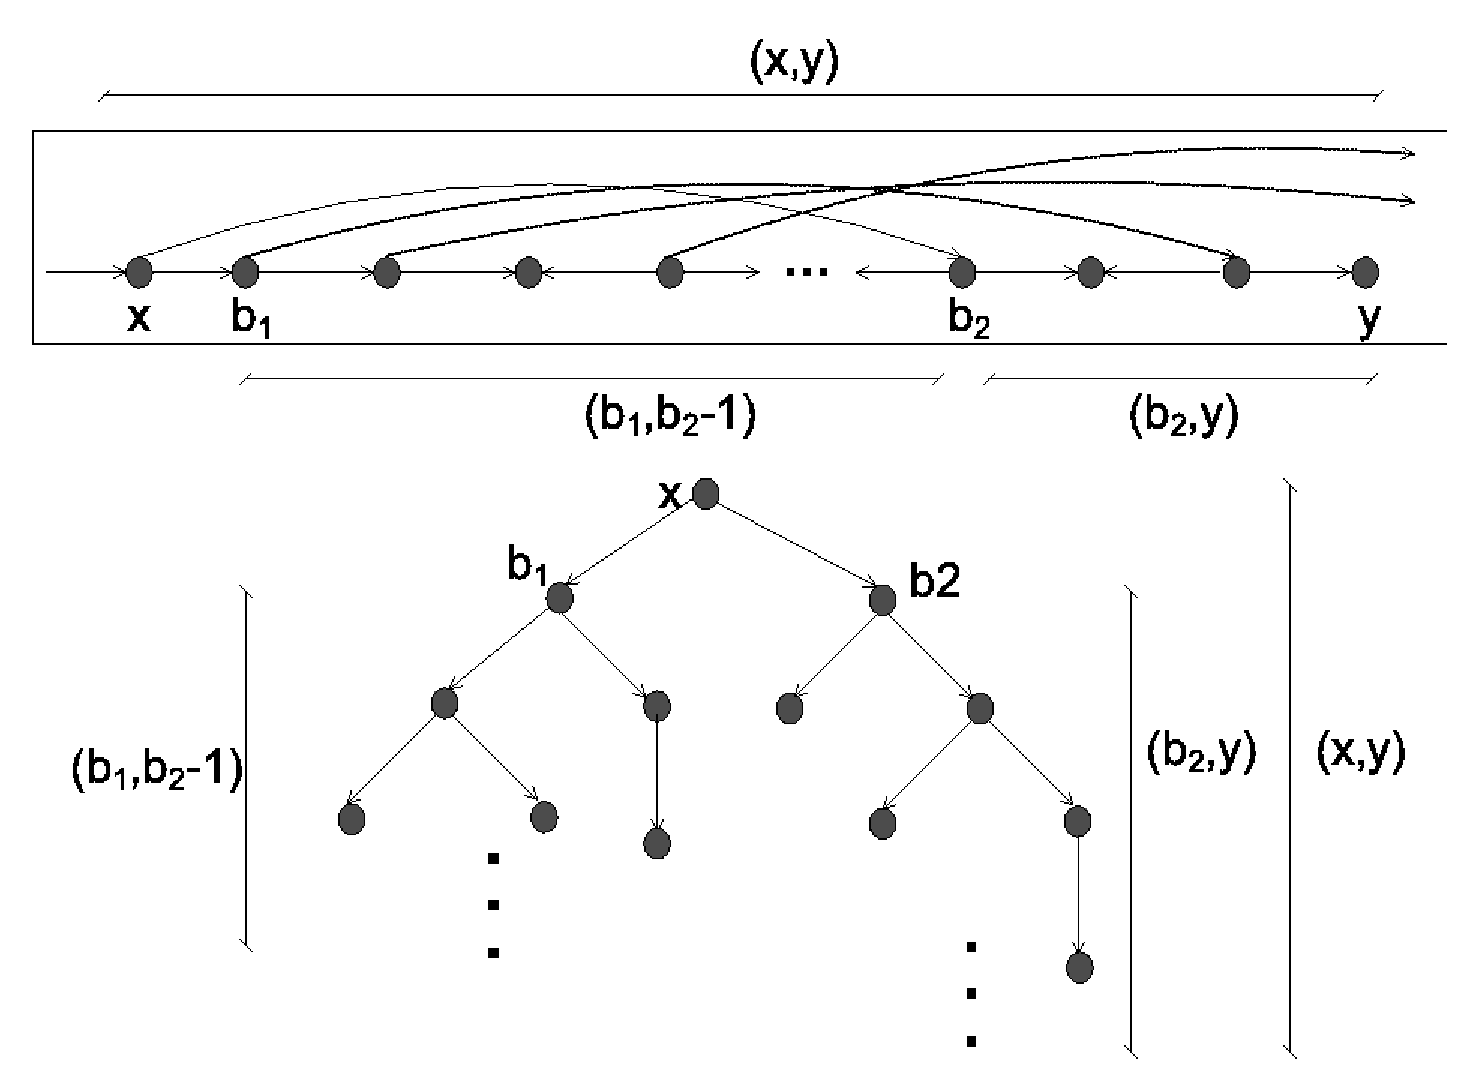
\includegraphics[width=4in]{figs/tree.eps}
\caption[Tree-based overlay broadcast]{Tree-based overlay broadcast}
\label{fig:tree}
\end{figure}  

Broadcast revocation can be used to address the deficiencies of DHT revocation.
As a topic of previous research works~\cite{broadcast, chord_broadcast},
structured overlays can be used without additional state to perform efficient
broadcasts from any point in the overlay to the entire overlay.  In these
papers, analysis and simulations have shown that the approach can be completed
in a network size of $n$ in $O(\log^2 n)$ time with $n$ messages.  The overlay
broadcast algorithm used in this paper provides a complete overlay broadcast in
$O(\log^2 n)$ time with $n$ messages.  When applied to Brunet, as illustrated
in Figure~\ref{fig:tree}, it utilizes the organization of a structured system
with a circular address space that requires peers be connected to those whose
node addresses are the closest to their own, features typical of
one-dimensional structured overlays including Chord~\cite{chord},
Pastry~\cite{pastry}, and Symphony.  Using such an organization, it is possible
to do perform a broadcast with no additional state.  To perform a broadcast,
each node performs the following recursive algorithm:

\begin{algorithmic}
\STATE {\bf BROADCAST(start, end, message)}:
  \STATE RECEIVE(message)
  \FOR{$i$ in length(connections)}
    \STATE n\_start $\gets$ ADDRESS(connections$[i]$)
    \IF {n\_start $\not\in$ $[$start, end$)$}
      \STATE continue
    \ENDIF
    \STATE n\_end $\gets$ ADDRESS(connections$[i+1]$)
    \IF {n\_end $\not\in$ $[$start, end$)$}
      \STATE n\_end $\gets$ end
    \ENDIF
    \STATE msg $\gets$ (BROADCAST, n\_start, n\_end, message)
    \STATE SEND(connections$[i]$, msg)
  \ENDFOR
\end{algorithmic}
with ``connections'' as a circular list of connections in non-decreasing order
from the perspective of the node performing the current recursive, broadcast
step.

In this algorithm, the broadcast initiator uses its own address as the start
and end, thus the broadcast will span the entire overlay after completing
recursive calls at each connected node.  A recursive end, ``n\_end'', must be
inside the region between ``start'' and ``end'', thus if the connection
following the current sending connection, ``connections$[i+1]$'', is not in
that region, it will only broadcast up to ``end'' and not the address specified
by that connection.  To summarize, the overlay is recursively partitioned
amongst the nodes at each hop in the broadcast.  By doing so, all nodes receive
the broadcast without receiving duplicate broadcast messages.

%If you have a single appendix, you need to change {\chapter*{APPENDIX: THIS IS THE FIRST APPENDIX}
%to {\chapter*{APPENDIX: YOUR APPENDIX TITLE HERE} if you have two or more appendices
%you need to change {\chapter{THIS IS THE FIRST APPENDIX}} to
%{\chapter{YOUR APPENDIX TITLE HERE}}
%
%If you make these changes correctly Latex will complain bitterly about the additions to the TOC
%but will make them correctly in a manner acceptable to the Editorial Office.

%\ifthenelse{\value{noa} = 1}
%...................then
%{\chapter*{APPENDIX: EVALUATION TOOLS}
%\label{evaluation_tools}
%\addcontentsline{toc}{chapter}{APPENDIX: EVALUATION TOOLS}
%\chaptermark{Appendix}
%\markboth{Appendix}{Appendix}
%\setcounter{chapter}{1}}
%...................else
{\chapter{EVALUATION TOOLS}
\label{evaluation_tools}}
%...................

Netperf~\cite{netperf} is used to estimate the latency and bandwidth of the
different VN models. The latency is measured by deploying Netperf in the
TCP\_RR mode, which measures the number of 1-byte request-receive transactions
that can be completed in a second. The bandwidth is estimated by running Netperf
in the TCP\_STREAM mode, which is a bulk transfer mode. It should be noted that
in situations where the link bandwidths were asymmetric, Netperf is deployed in
both directions.  Since both latency and bandwidth are dependent on the CPU
comparison, evaluations that include CPU utilization tasks require creating
a baseline first where only Netperf is the only active workload.

SPECjbb~\cite{specjbb} simulates a three-tier web application with all the
clients, the middle tier, and the database running on a single system in a
single address space (inside a JVM). On completion, the benchmark provides the
metric in terms of business of operations per second (bops). The bops score of
the system under test depends on both the CPU and the memory in the system, as
the entire database for the benchmark is held in memory. This benchmark
generates negligible disk activity and no network activity. 



%------------------------------------------%

% Make List of References (BibTeX implemented using the Natbib package)
% un-comment your preferred bibliography style and replace the
% bibliography file "sample" with the name of your .bib file
% REMEMBER!!! If you want un-numbered references comment the Natbib package with
% The numbered options in the packages.tex file and un-comment the package with the authoryear option
% See the included pdfs of the various styles to see the differences.
% The citation style differences are from the \citet{key} and \citep{key} commands
% More options are available; see the Natbib documentation for details


\bibliography{ufsampleETD}
% You can have more than one library of references
%------------------------------------------%

% Bio Sketch %
% Just type your bio in between the brackets
\biography{%

David Isaac Wolinsky was born on October 31, 1982.  He was blessed with an
awesome, Isaac Emmanuel, born November 30, 2009.  Beginning his studies in
August 2001 at the University of Florida, David obtained the following degrees
in electrical and computer engineering: Bachelor of Science in Spring 2005,
Master of Science in Spring 2007, and Doctorate of Philosophy in Summer 2011.
His advisor at the University of Florida was Professor Renato Figueiredo, whom
he began working with since the during the Spring of 2006 at the Advanced
Computing and Information Systems Lab.

His primary research focuses are network virtualization using structured P2P
(peer-to-peer) overlays and grid computing.  The networking research has been
realized in IPOP, a free (BSD - Berkeley Software Distribution licence))
network virtualization software.  Additionally, he has worked on enabling DHTs,
decentralized NAT (network address translation) traversal through relays,
software models for improved network virtualization, and autonomic virtual
networking stacks.  This work is a major contribution to his grid computing
research focus, Grid Appliance, which enables the creation of decentralized,
distributed grids using virtualized, physical, and cloud resources.  Going
forward, he expressed great interested in using these concepts in other
distributed systems such as sensor networks, social networks, cloud services,
or even web services.

During his free time, he enjoys time with my boy, running, playing basketball,
and occasionally playing video games.  At one point, he was ranked in the top
20 on the US East Warcraft III Free For All Ladder.  

}


%------------------------------------------%

\end{document}

%-------------------------------------------------------------------------------------------------------%
